\section{Supplementary DQM example plots}
\begin{figure}[htbp]
  \centering
      \subfigure[$\phi_{E_{T,miss}}$]{
    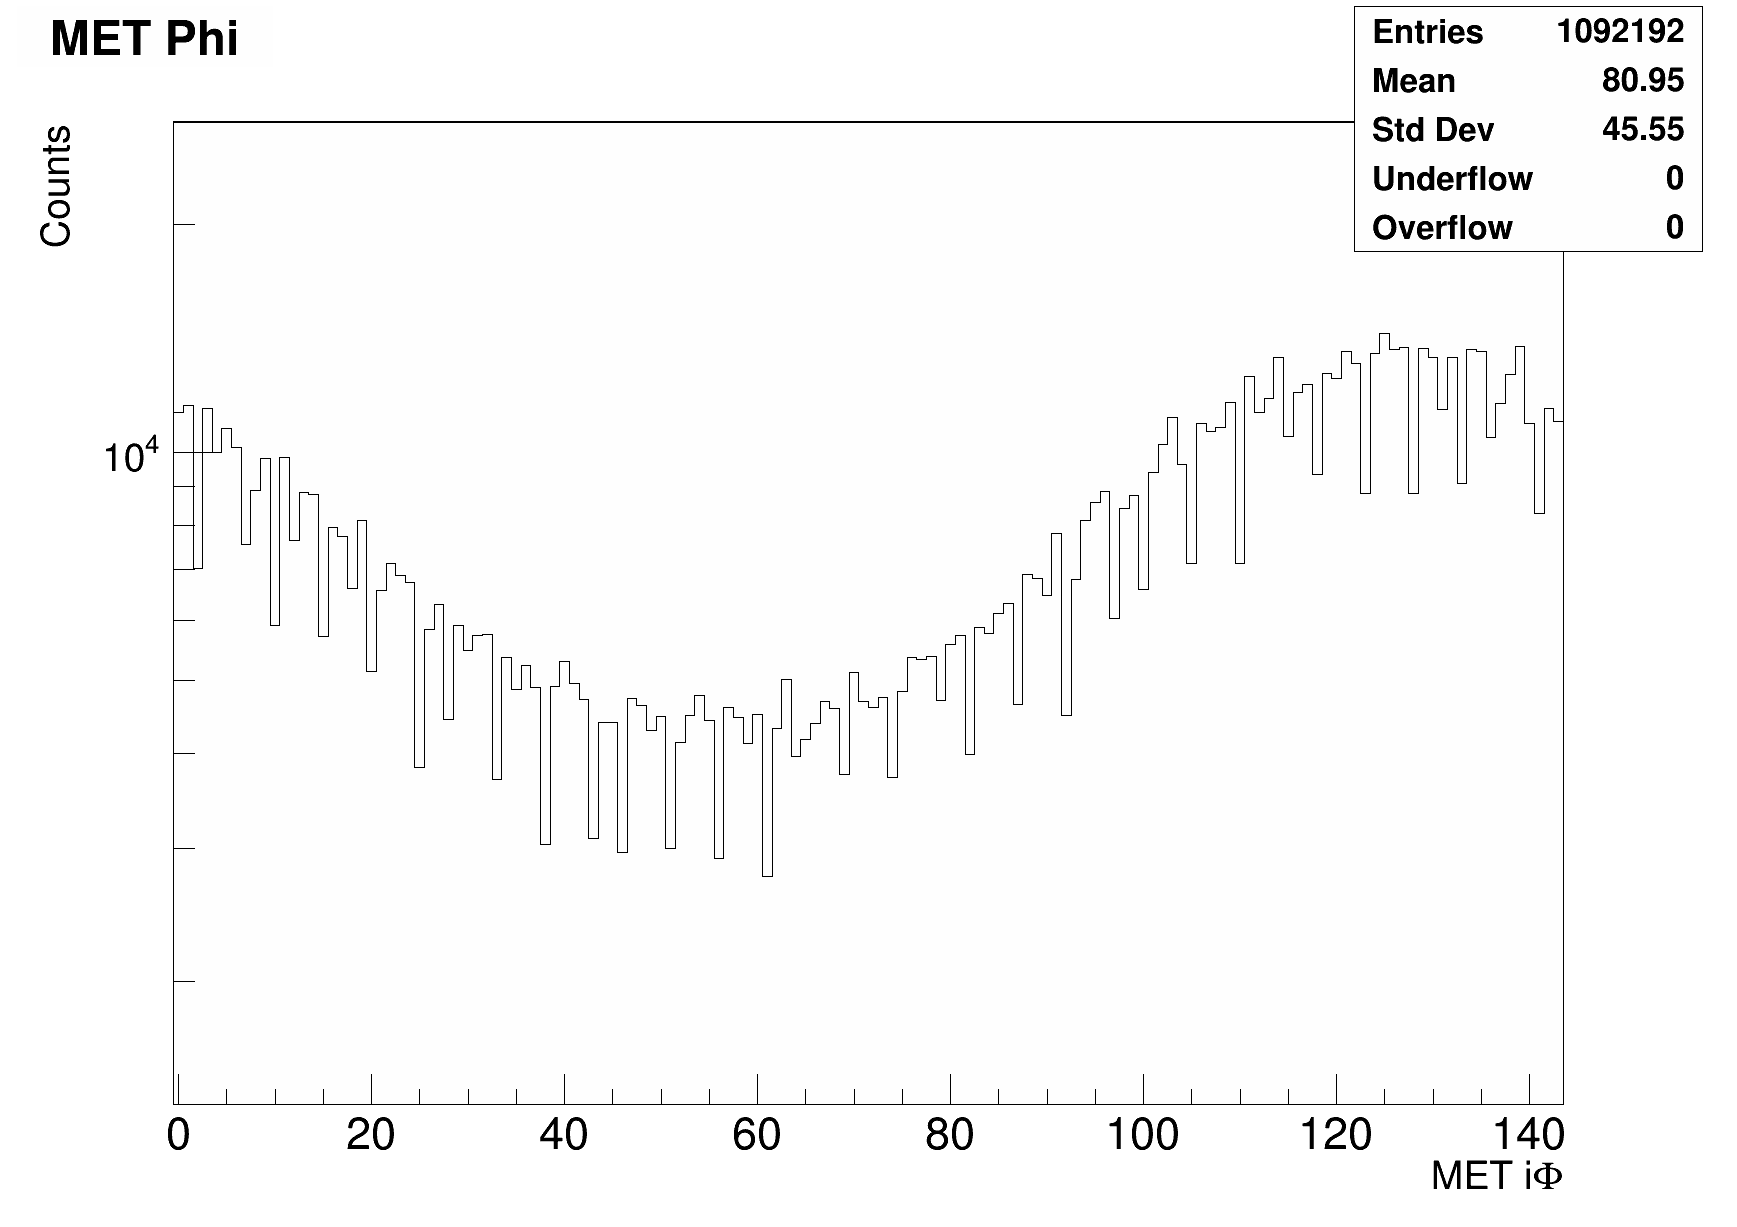
\includegraphics[width=0.47\textwidth]{CMS_experiment/METPhi.png}
    }
    \subfigure[$\phi_{H_{T,miss}}$]{
    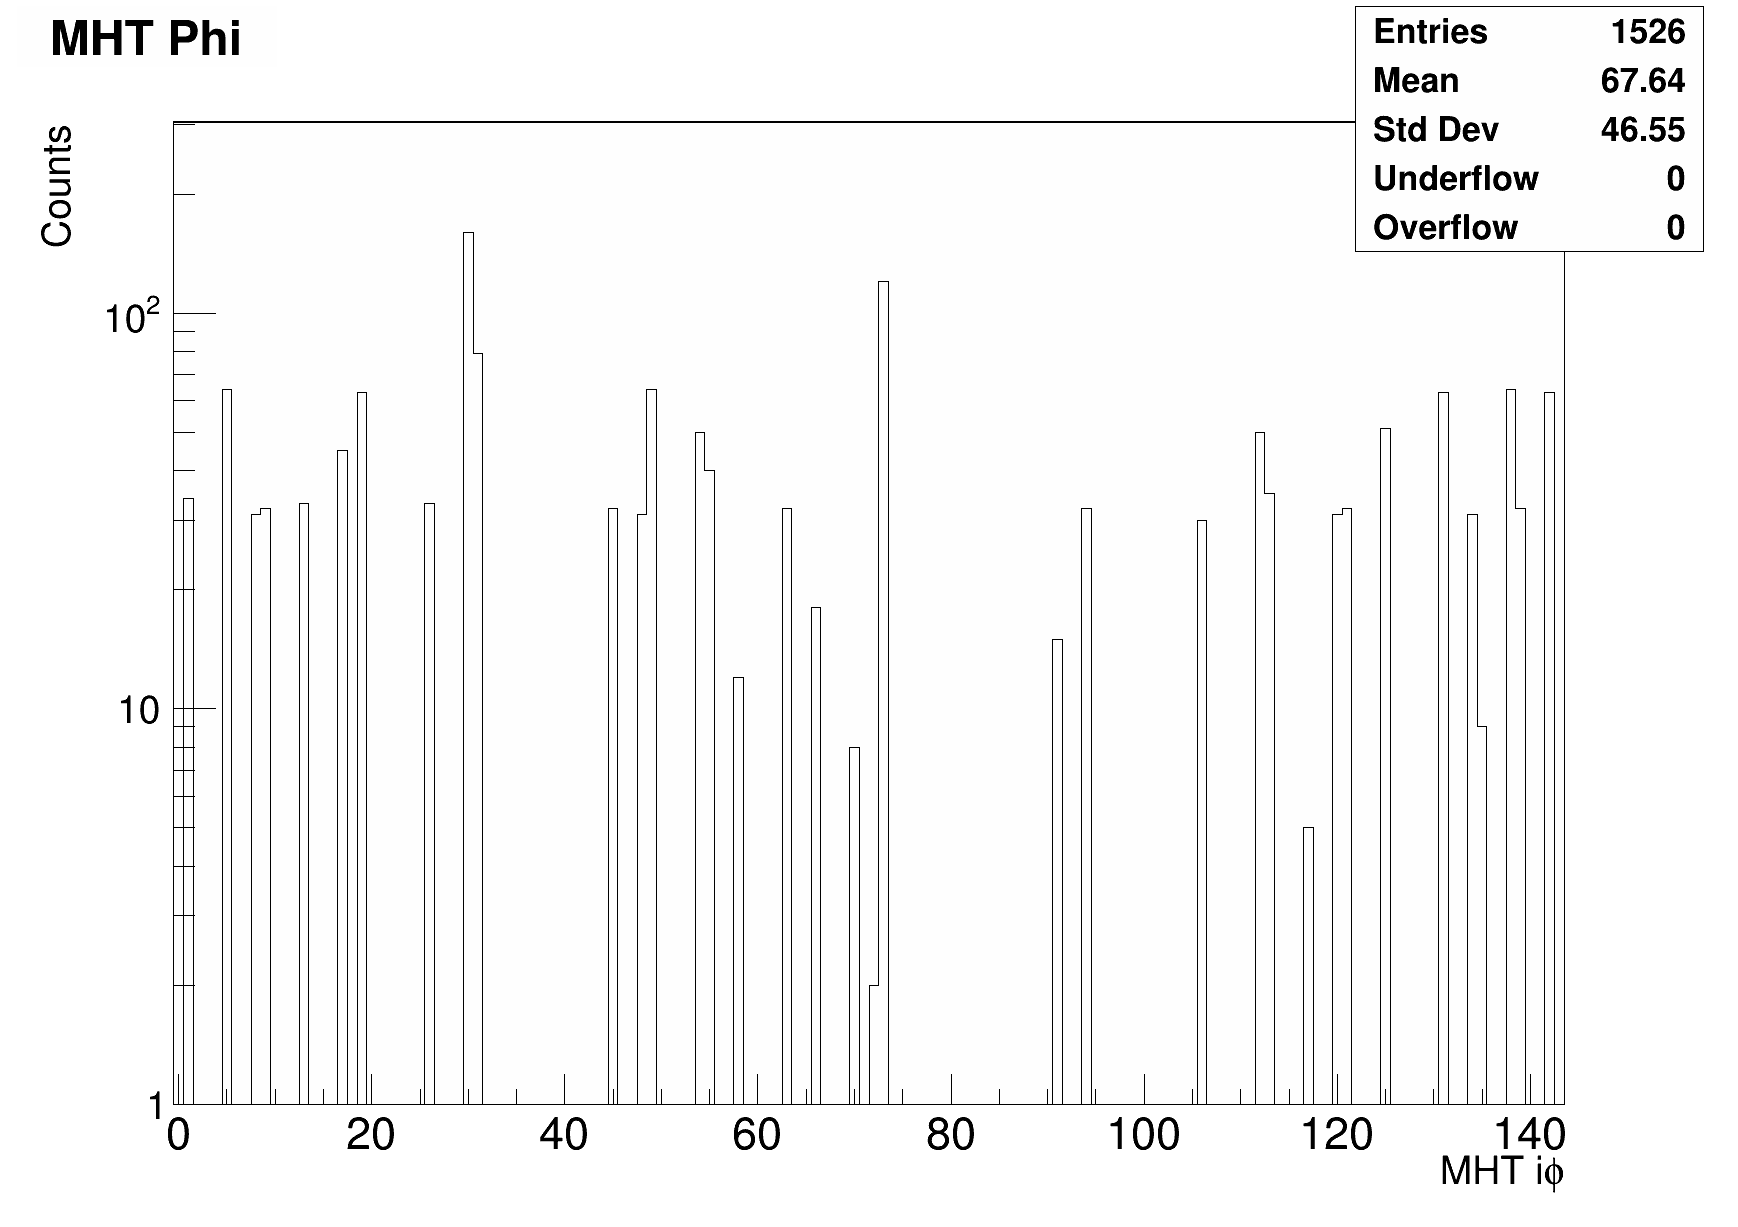
\includegraphics[width=0.47\textwidth]{CMS_experiment/MHTPhi.png}
    }\\
    \subfigure[Asymmetry]{
    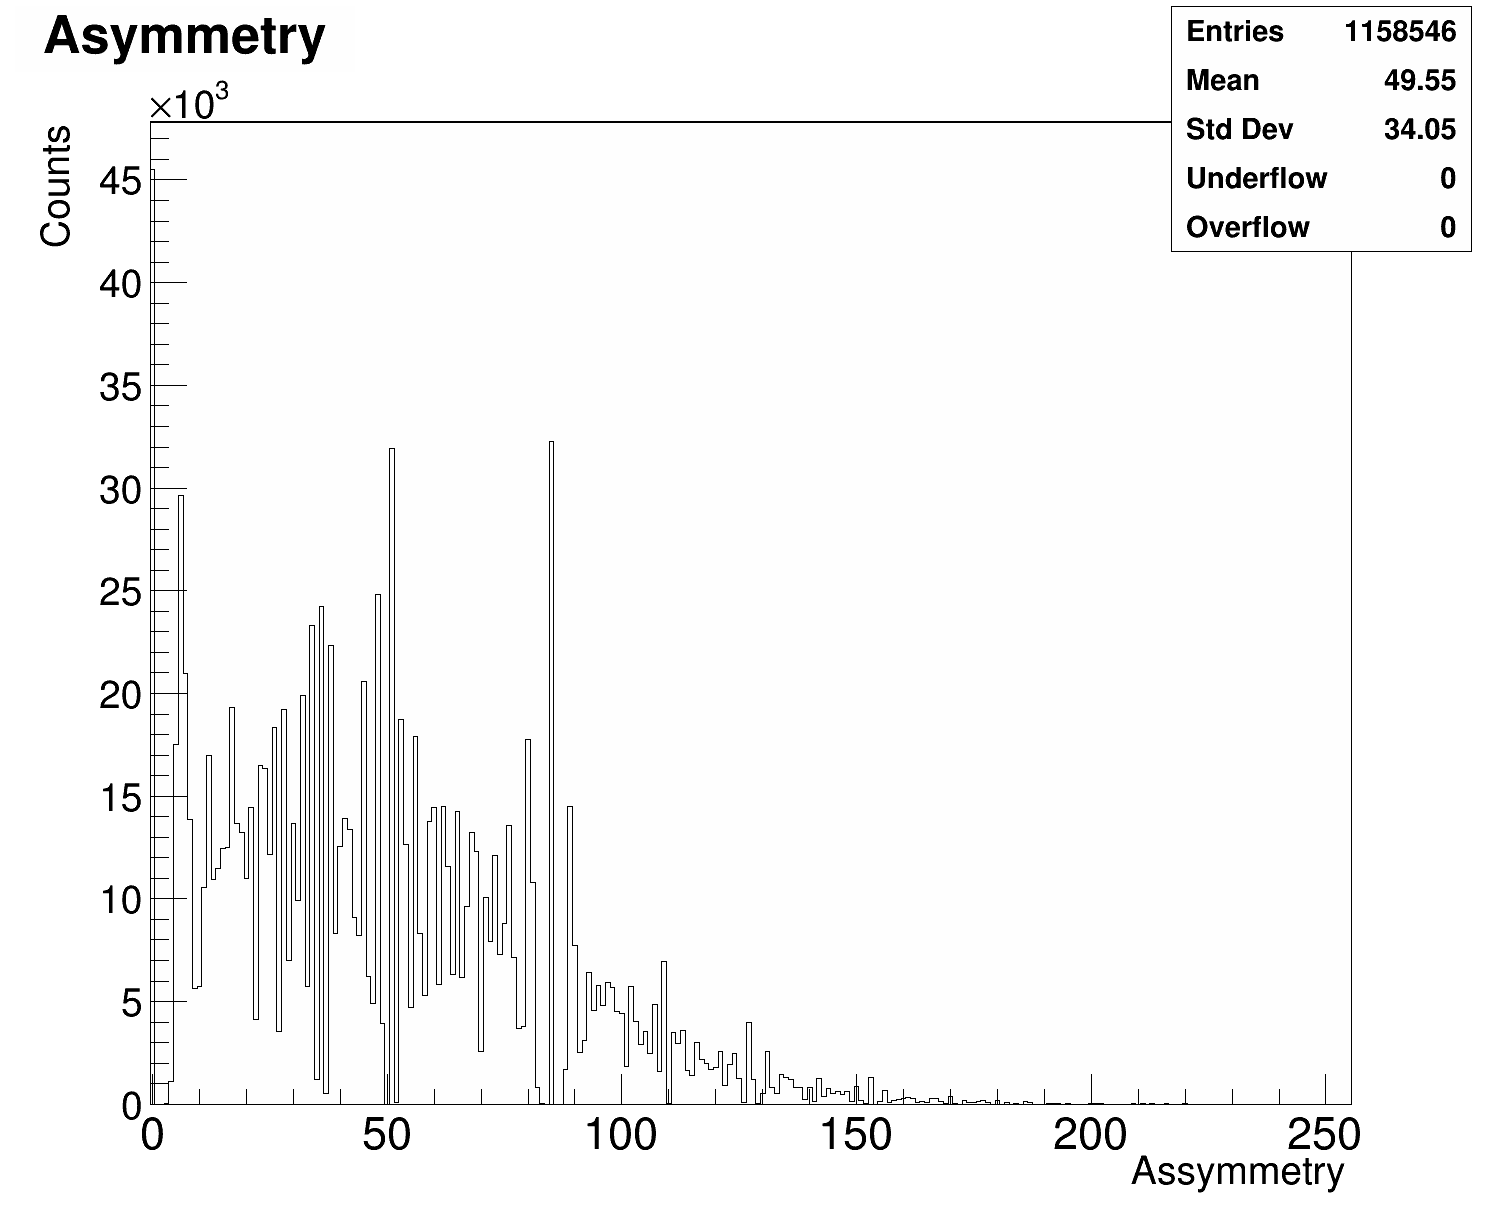
\includegraphics[width=0.47\textwidth]{CMS_experiment/Asymmetry.png}
    }
    \subfigure[Centrality]{
    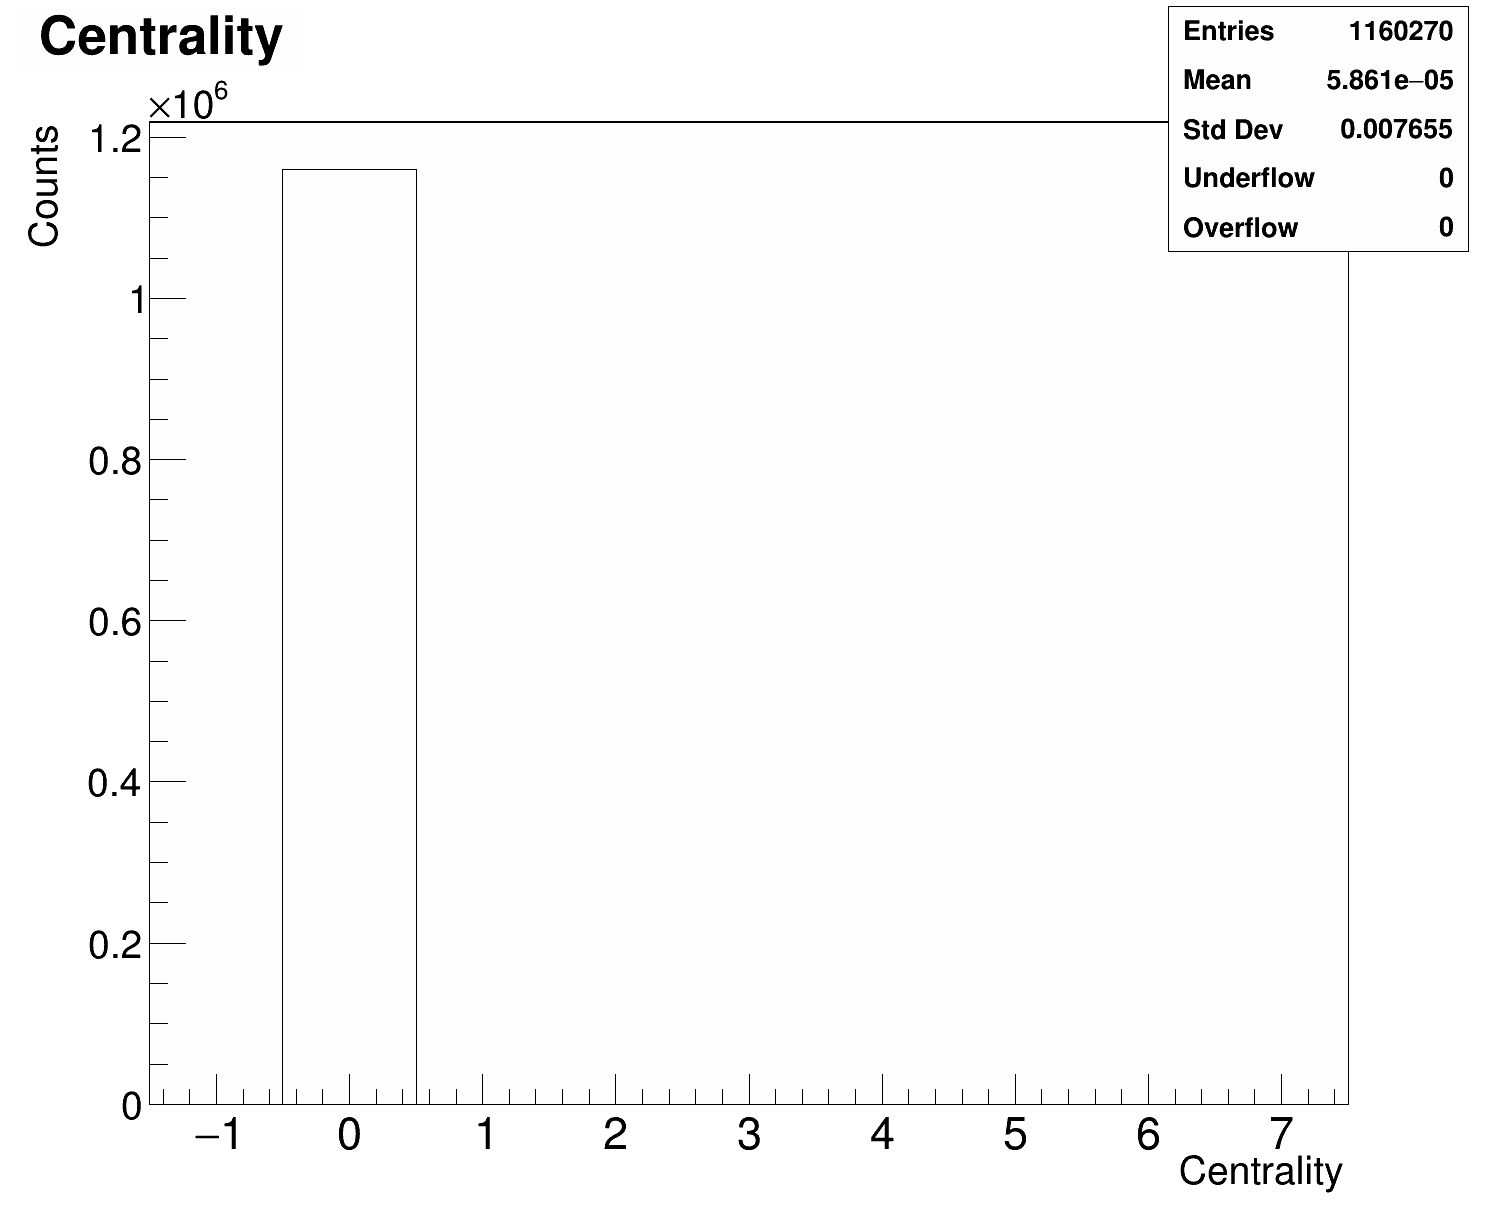
\includegraphics[width=0.47\textwidth]{CMS_experiment/Centrality.png}
    }%\\
  %  \subfigure[High level comparison summary ]{
  %  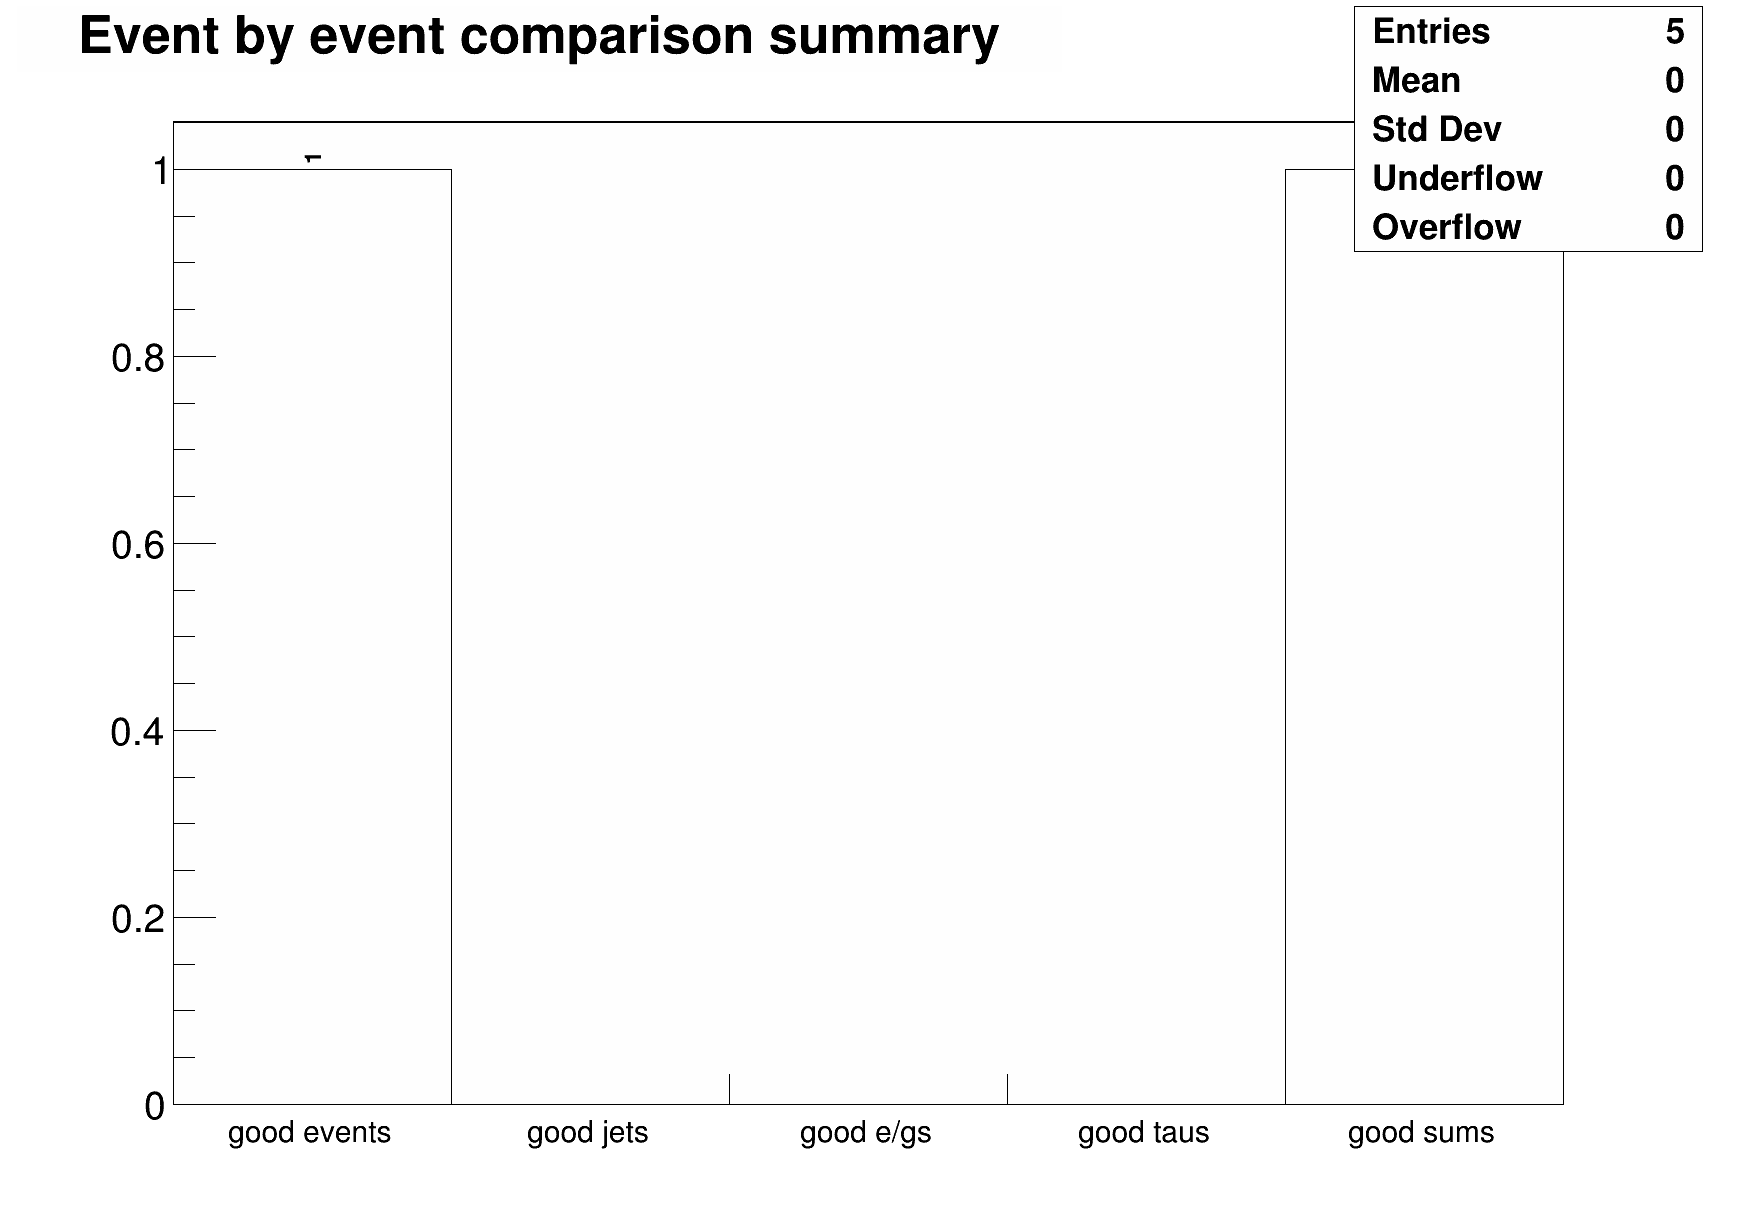
\includegraphics[width=0.45\textwidth]{CMS_experiment/High_level_summary.png}
  %  }
  %  \subfigure[Summary of problematic events]{
  %  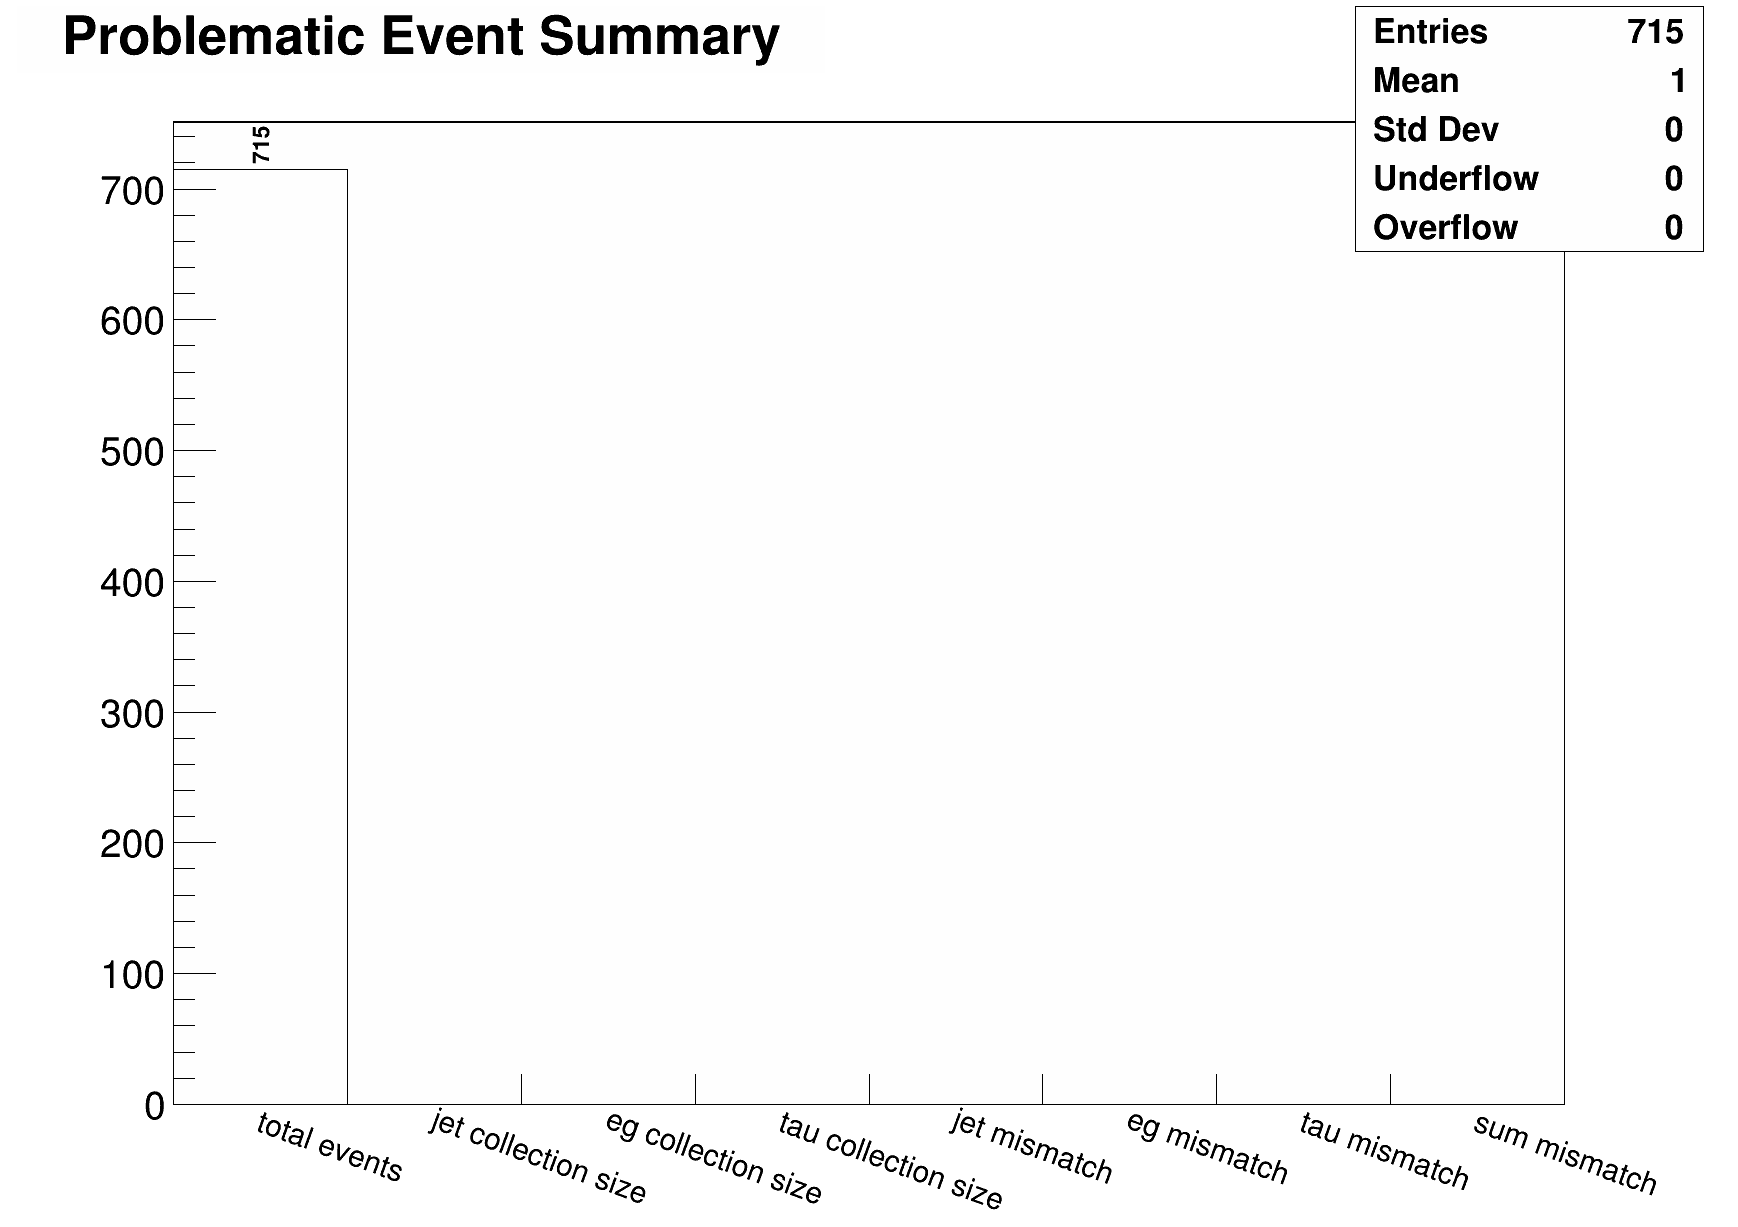
\includegraphics[width=0.45\textwidth]{CMS_experiment/Problem_Summary.png}
  %  }
  \caption{DQM example distributions showing the: (a) $\phi$ of the $\vec{p}_{T,miss}$, (b) $\phi$ of the $\vec{H}_{T,miss}$, (c) asymmetry and (d) centrality variables.}
  \label{app:dqm_plots}
\end{figure}
\newpage


\section{List of triggers used in the analysis}
\label{app:trigger_list}
\hspace{10pt} Table~\ref{a_tab:triggers} shows the list of HLT algorithms used in the analysis. The corresponding input L1 seeds are listed for each HLT path, with the separation being made for each era of data taking in order to present different thresholds for each year.

\begin{table}[htbp]

    \centering
     \def\arraystretch{1.5}

    \tiny

    \begin{tabular}{l l c}
        \hline\hline
        Year                   & HLT path                                                  & L1 seed                                 \\\hline\hline
        \multirow{8}{*}{2017}  & HLT\_PFMETNoMu120\_PFMHTNoMu120\_IDTight                  & \texttt{L1\_ETMHF70}                     \\
                               & HLT\_PFMETNoMu120\_PFMHTNoMu120\_IDTight\_PFHT60          & \texttt{L1\_ETMHF80\_HTT60er }                      \\\cline{2-3}
                               & HLT\_Ele35\_WPTight\_Gsf                                  & \texttt{L1\_SingleEG24}                     \\\cline{2-3}
                               & \multirow{3}{*}{HLT\_Photon200}                           & \texttt{L1\_SingleEG30}         \\
                               &                                                           & \texttt{L1\_SingleJet170}        \\
                               &                                                           & \texttt{L1\_SingleTau100er2p1}                  \\\cline{2-3}
                               & HLT\_DiJet110\_35\_Mjj650\_PFMET110                       & \texttt{L1\_DoubleJet\_*\_*\_DoubleJet*\_Mass\_Min620}             \\\cline{2-3}
                               & HLT\_TripleJet110\_35\_35\_Mjj650\_PFMET110               & \texttt{L1\_DoubleJet\_*\_*\_DoubleJet*\_Mass\_Min620}     
                               \\\hline\hline

        \multirow{15}{*}{2018} & \multirow{2}{*}{HLT\_PFMETNoMu120\_PFMHTNoMu120\_IDTight} & \texttt{L1\_ETMHF100}                    \\
                               &                                                           & \texttt{L1\_ETM150}                                           \\
                               & HLT\_PFMETNoMu120\_PFMHTNoMu120\_IDTight\_PFHT60          & \texttt{L1\_ETMHF90\_HTT60er}                                 \\\cline{2-3}
                               & \multirow{3}{*}{HLT\_Ele32\_WPTight\_Gsf}                 & \texttt{L1\_SingleIsoEG24er2p1}      \\
                               &                                                           & \texttt{L1\_SingleEG26er2p5}                                   \\
                               &                                                           & \texttt{L1\_SingleEG60}                                        \\\cline{2-3}

                               & \multirow{5}{*}{HLT\_Photon200}                           & \texttt{L1\_SingleEG34er2p5}          \\
                               &                                                           & \texttt{L1\_SingleJet160er2p5}                                 \\
                               &                                                           & \texttt{L1\_SingleJet180}                                      \\
                               &                                                           & \texttt{L1\_SingleTau120er2p1}                                 \\
                               &                                                           & \texttt{L1\_SingleEG60}                                        \\\cline{2-3}
                               & \multirow{2}{*}{HLT\_DiJet110\_35\_Mjj650\_PFMET110}      & \texttt{L1\_DoubleJet\_*\_*\_DoubleJet*\_Mass\_Min620}         \\
                               &                                                      & \texttt{L1\_DoubleJet\_*\_*\_DoubleJet*\_Mass\_Min620\_Jet60TT28} 
                               \\\cline{2-3}
                               & \multirow{2}{*}{HLT\_TripleJet110\_35\_35\_Mjj650\_PFMET110} & \texttt{L1\_DoubleJet\_*\_*\_DoubleJet*\_Mass\_Min620}  \\
                               &                                                             & \texttt{L1\_DoubleJet\_*\_*\_DoubleJet*\_Mass\_Min620\_Jet60TT28}  \\\hline


        \hline\hline %--------------------------------------------------------------------------------------------------------------------------      \
    \end{tabular}
    \caption{List of HLT paths accompanied by the corresponding L1 seeds used as input~\cite{note:AN_19_257}.
    During the 2017 era the L1\_DoubleJet seeds imposed thresholds for leading jet $p_T$ threshold ranging from 90 to 115~GeV, while the subleading jet threshold took values from 30 to 40~GeV.
    Similarly for the 2018 data taking period, the L1\_DoubleJet seeds required the leading jet $p_T$ threshold range from 90 to 120~GeV and the subleading jet $p_T$ minimum value ranging from 30 to 45~GeV.}
    \label{a_tab:triggers}

\end{table}

\newpage
\section{Analysis strategy for the 2018 era}
\label{app:MTR_2018}
\hspace{10pt} Figure~\ref{fig:2018_SR_motivation_1} shows the distributions of main analysis variables in the SR after the full MTR selection being applied, for the 2018 era. The corresponding distributions for the VTR category are given in Figure~\ref{fig:2018_VTR_SR_motivation_1}.

\begin{figure}[htbp]
  \centering
      \subfigure[$E_{T,miss}$]{
    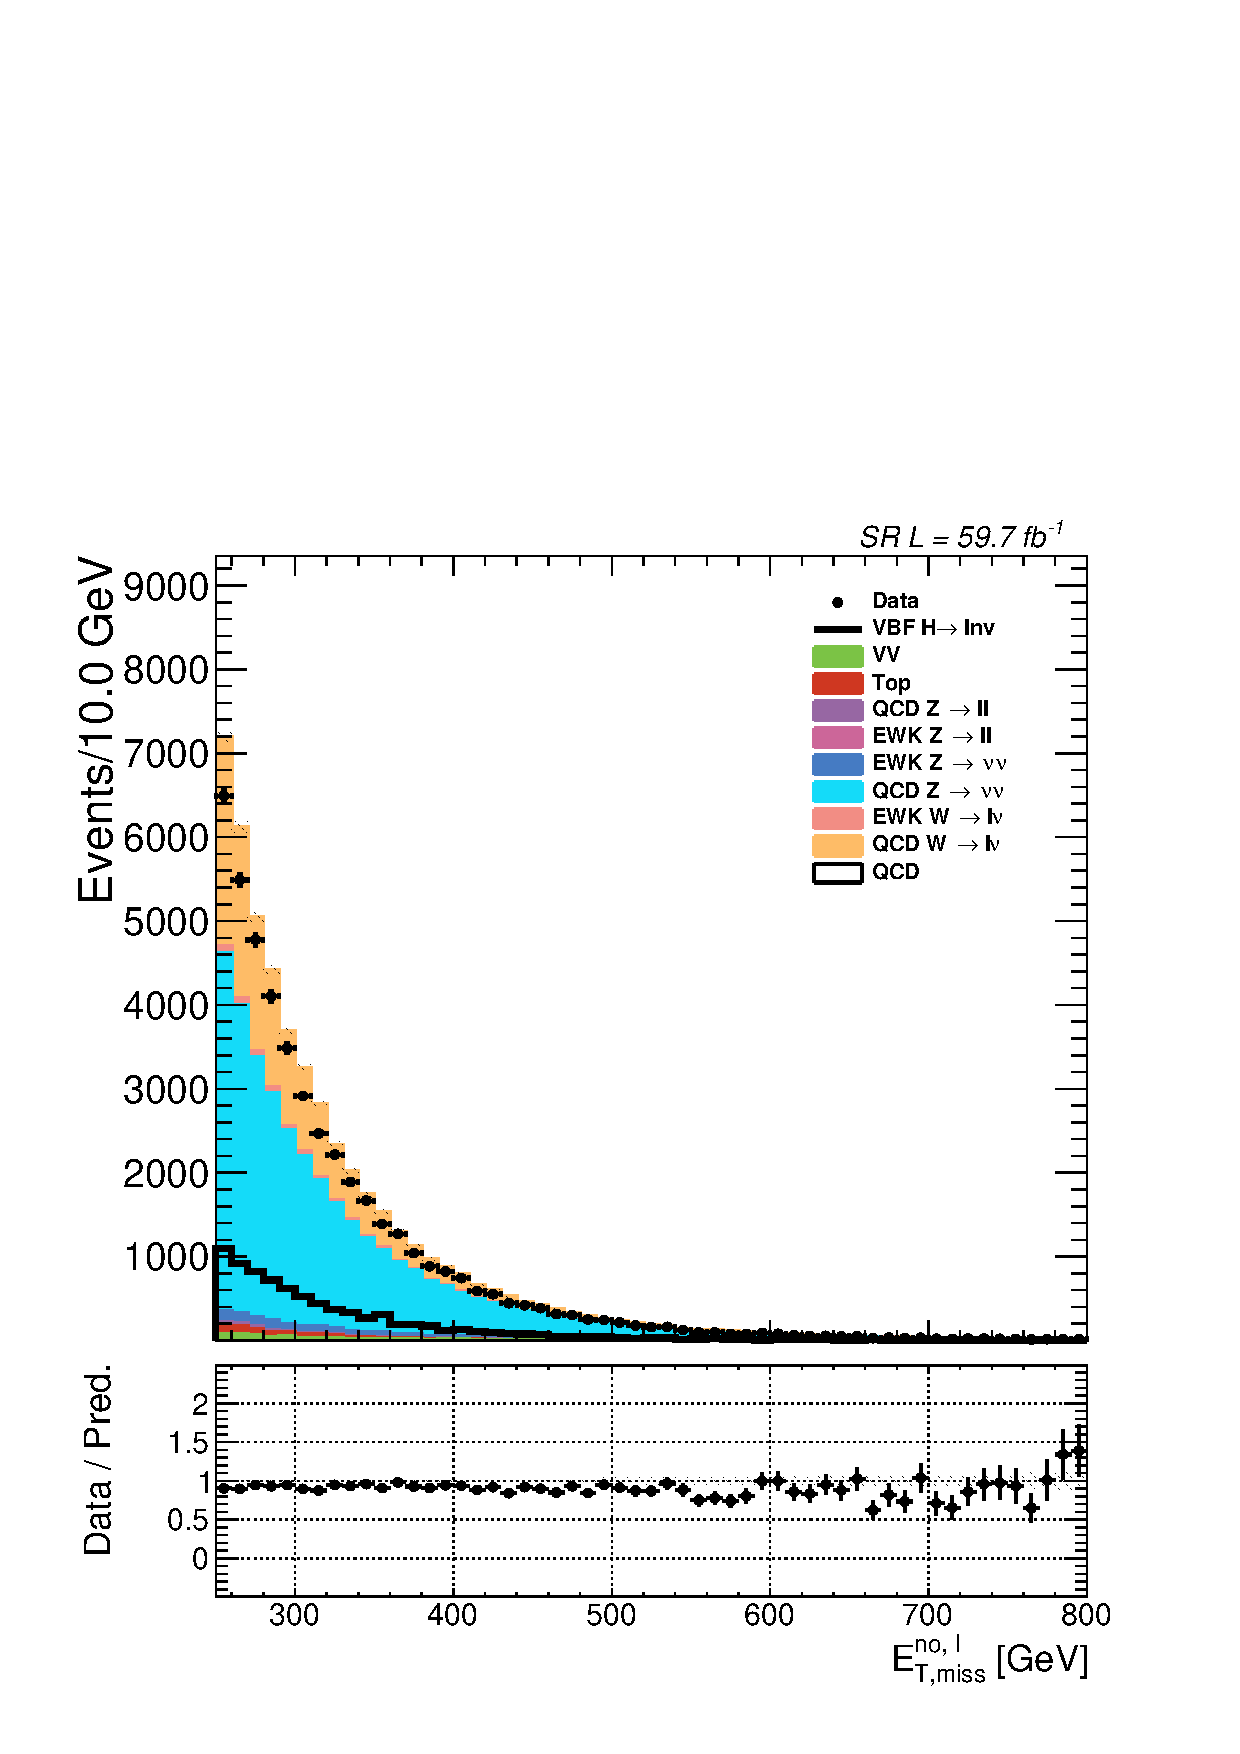
\includegraphics[width=0.49\textwidth]{Analysis_strategy/MTR_2018_SR/MetNoMu.pdf}
    }
    \subfigure[$m_{jj}$]{
    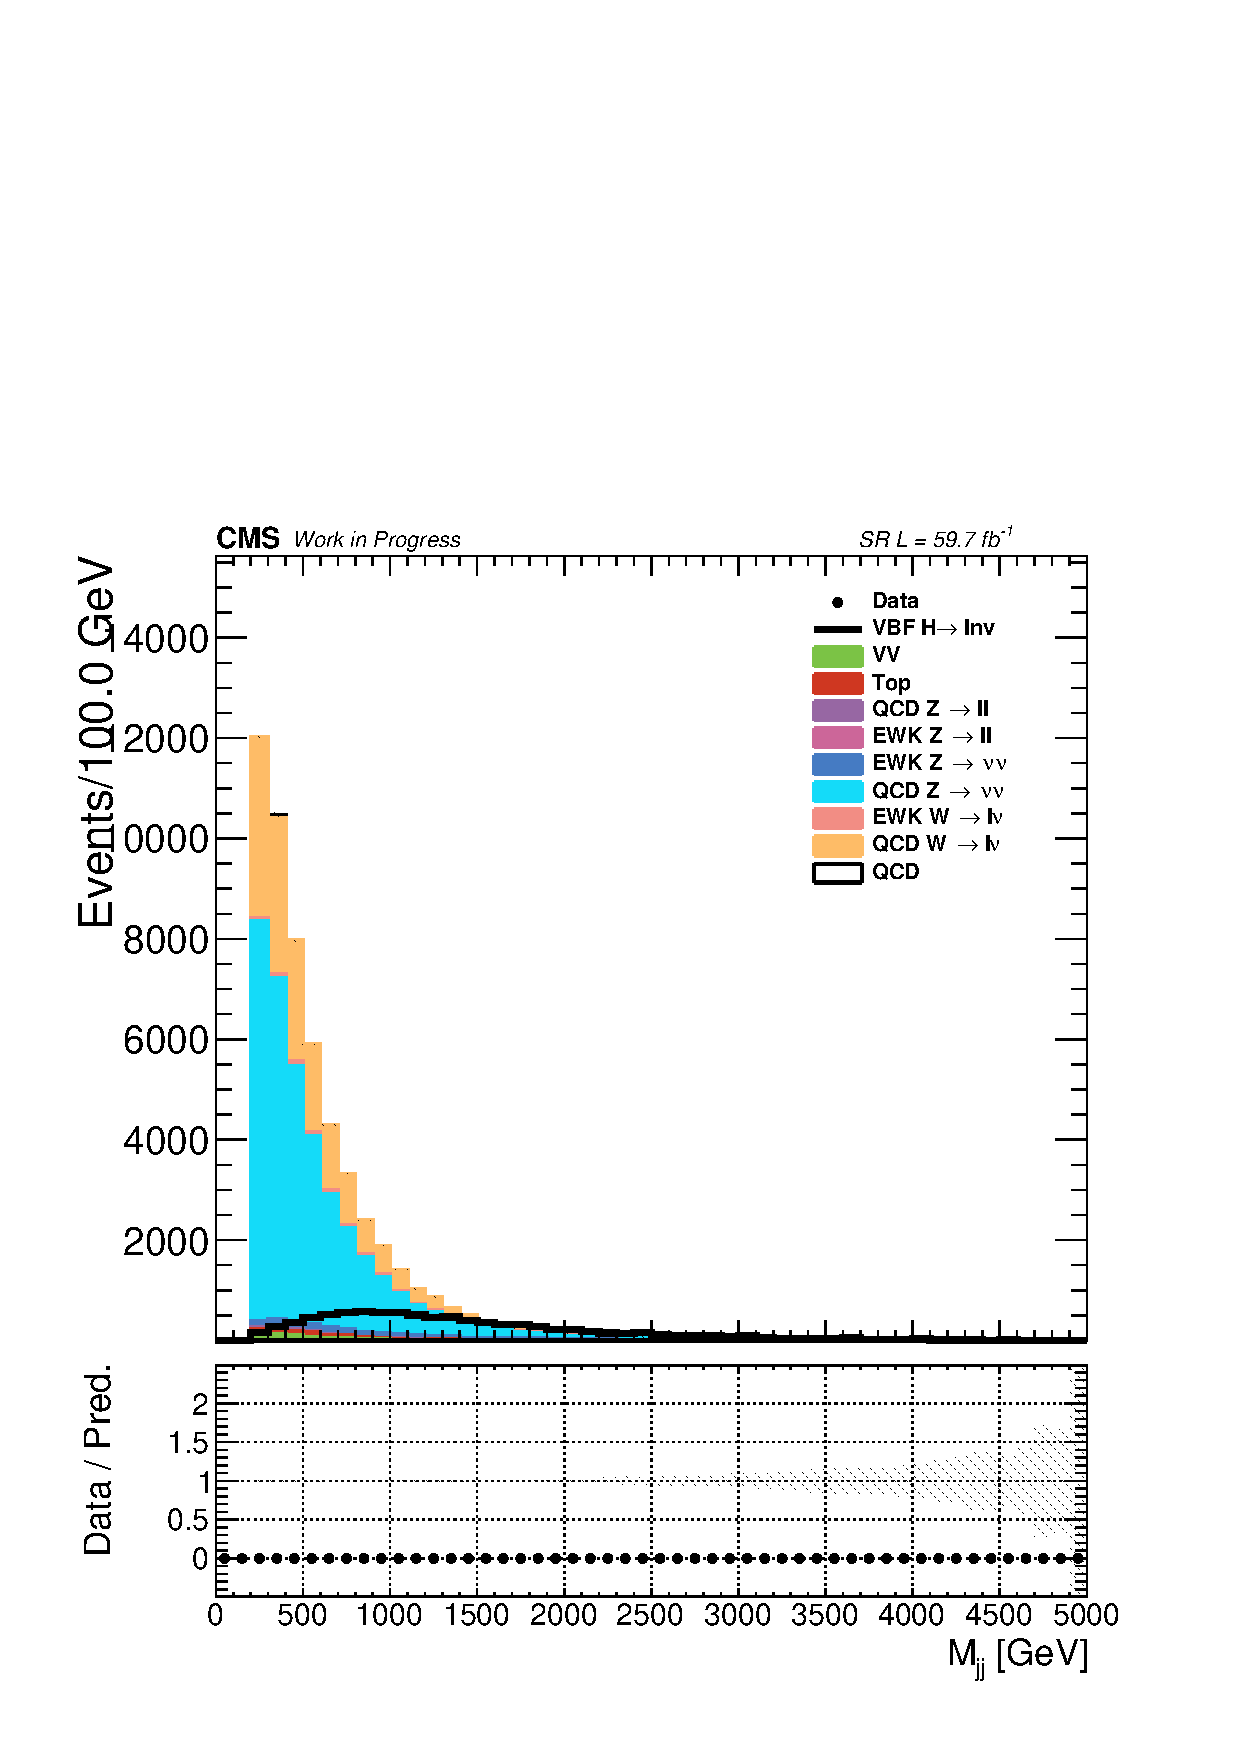
\includegraphics[width=0.49\textwidth]{Analysis_strategy/MTR_2018_SR/leadingJet_mjj.pdf}
    }\\
    \subfigure[$\Delta\eta_{jj}$]{
    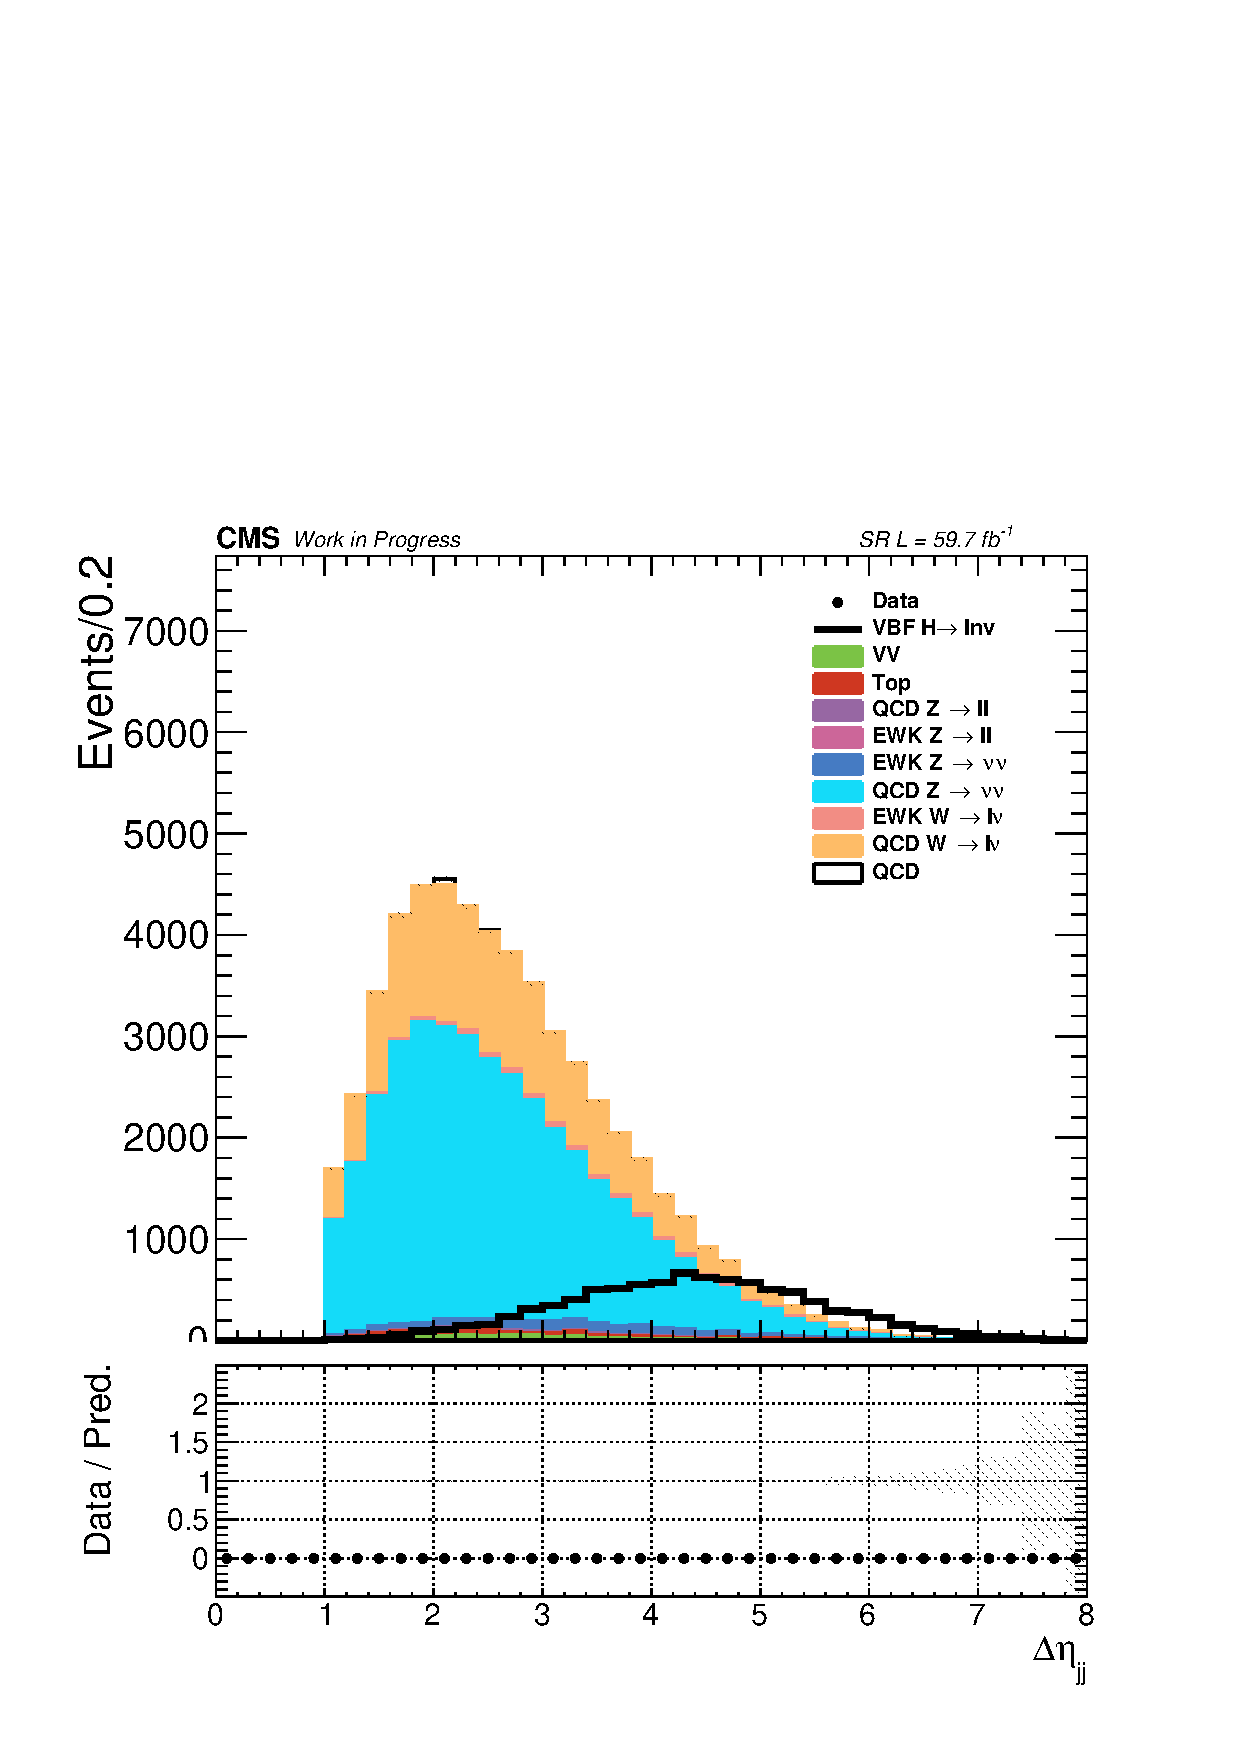
\includegraphics[width=0.49\textwidth]{Analysis_strategy/MTR_2018_SR/leading_dEtajj.pdf}
    }
    \subfigure[$\Delta\phi_{jj}$]{
    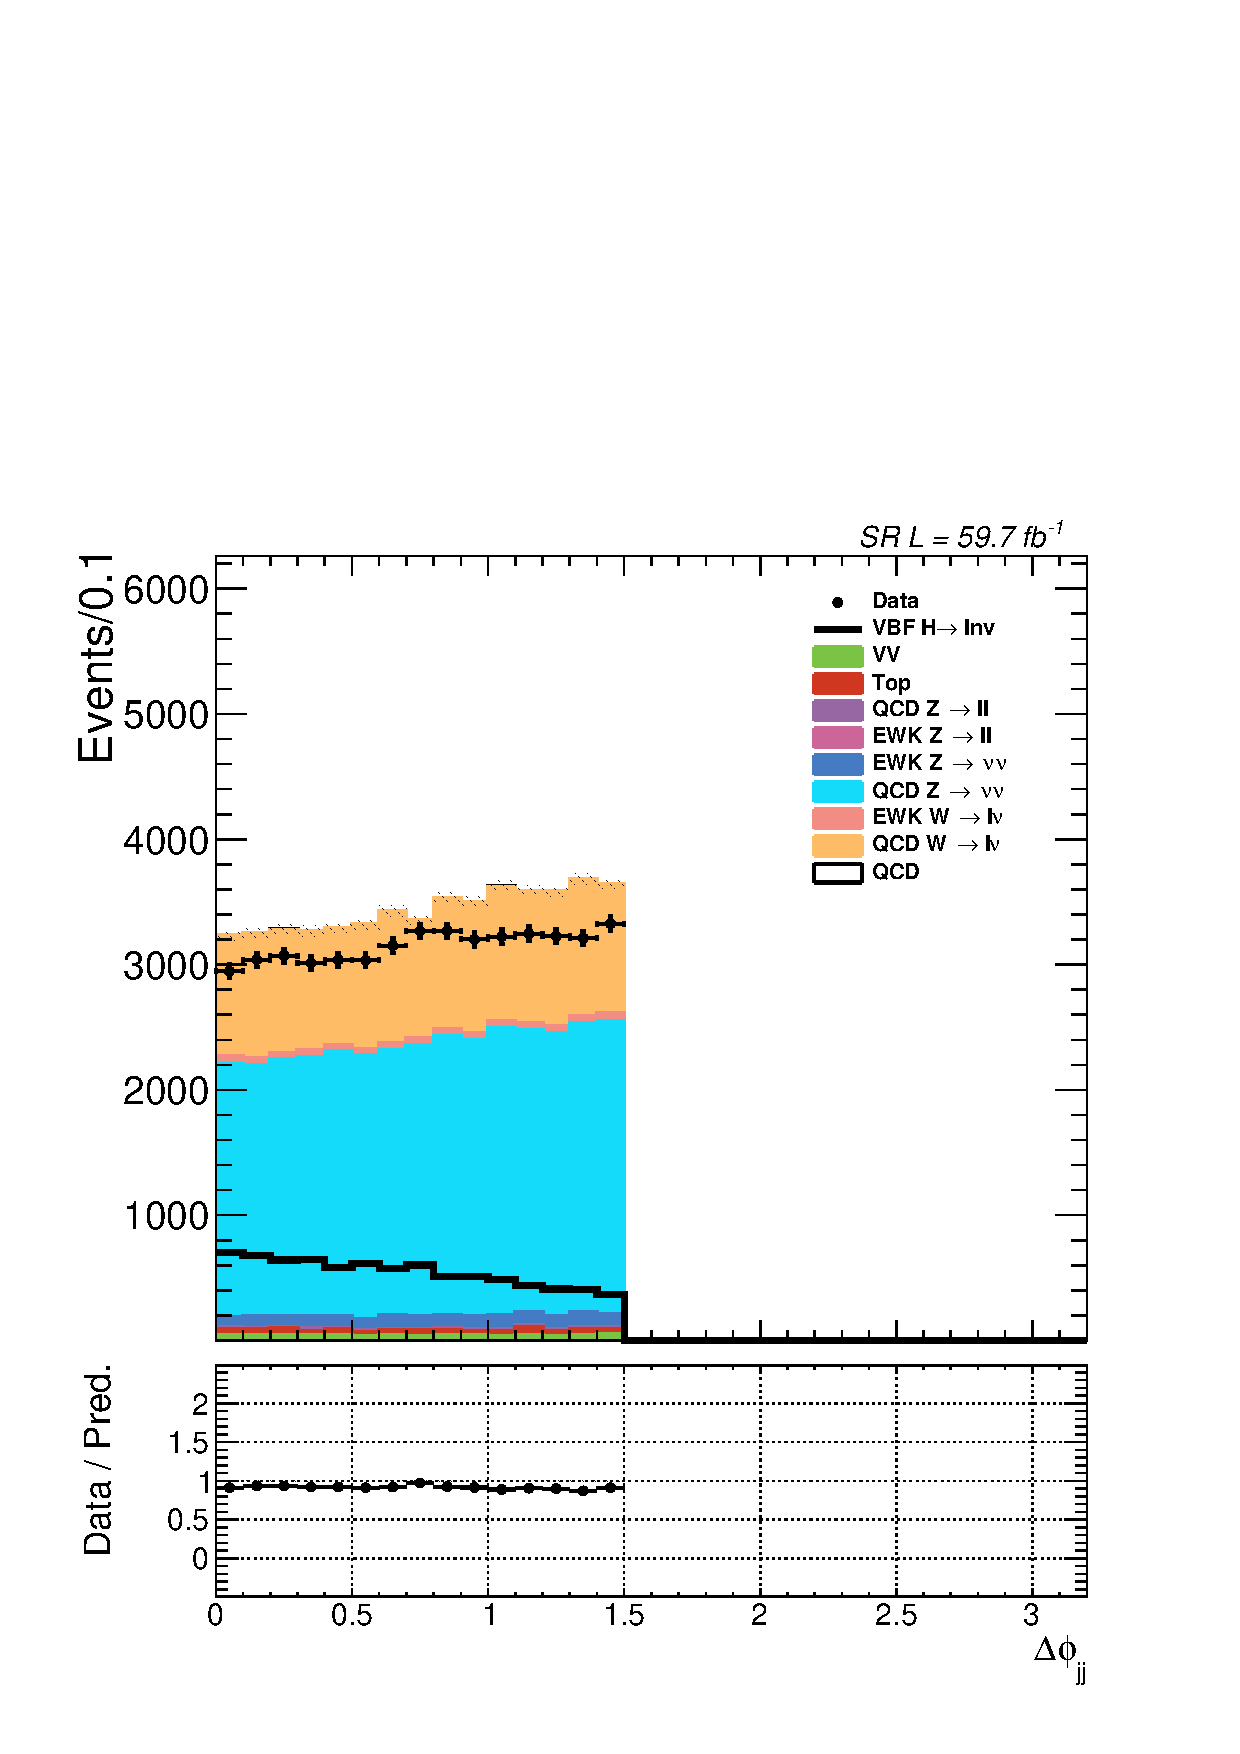
\includegraphics[width=0.49\textwidth]{Analysis_strategy/MTR_2018_SR/leading_dPhijj.pdf}
    }
  \caption{Distributions of $E_{T,miss}$, $m_{jj}$, $\Delta\eta_{jj}$ and $\Delta\phi_{jj}$ variables in the SR after the full MTR selection, for 2018 data.}
  \label{fig:2018_SR_motivation_1}
\end{figure}


%\newpage



\begin{figure}[htbp]
  \centering
      \subfigure[$E_{T,miss}$]{
    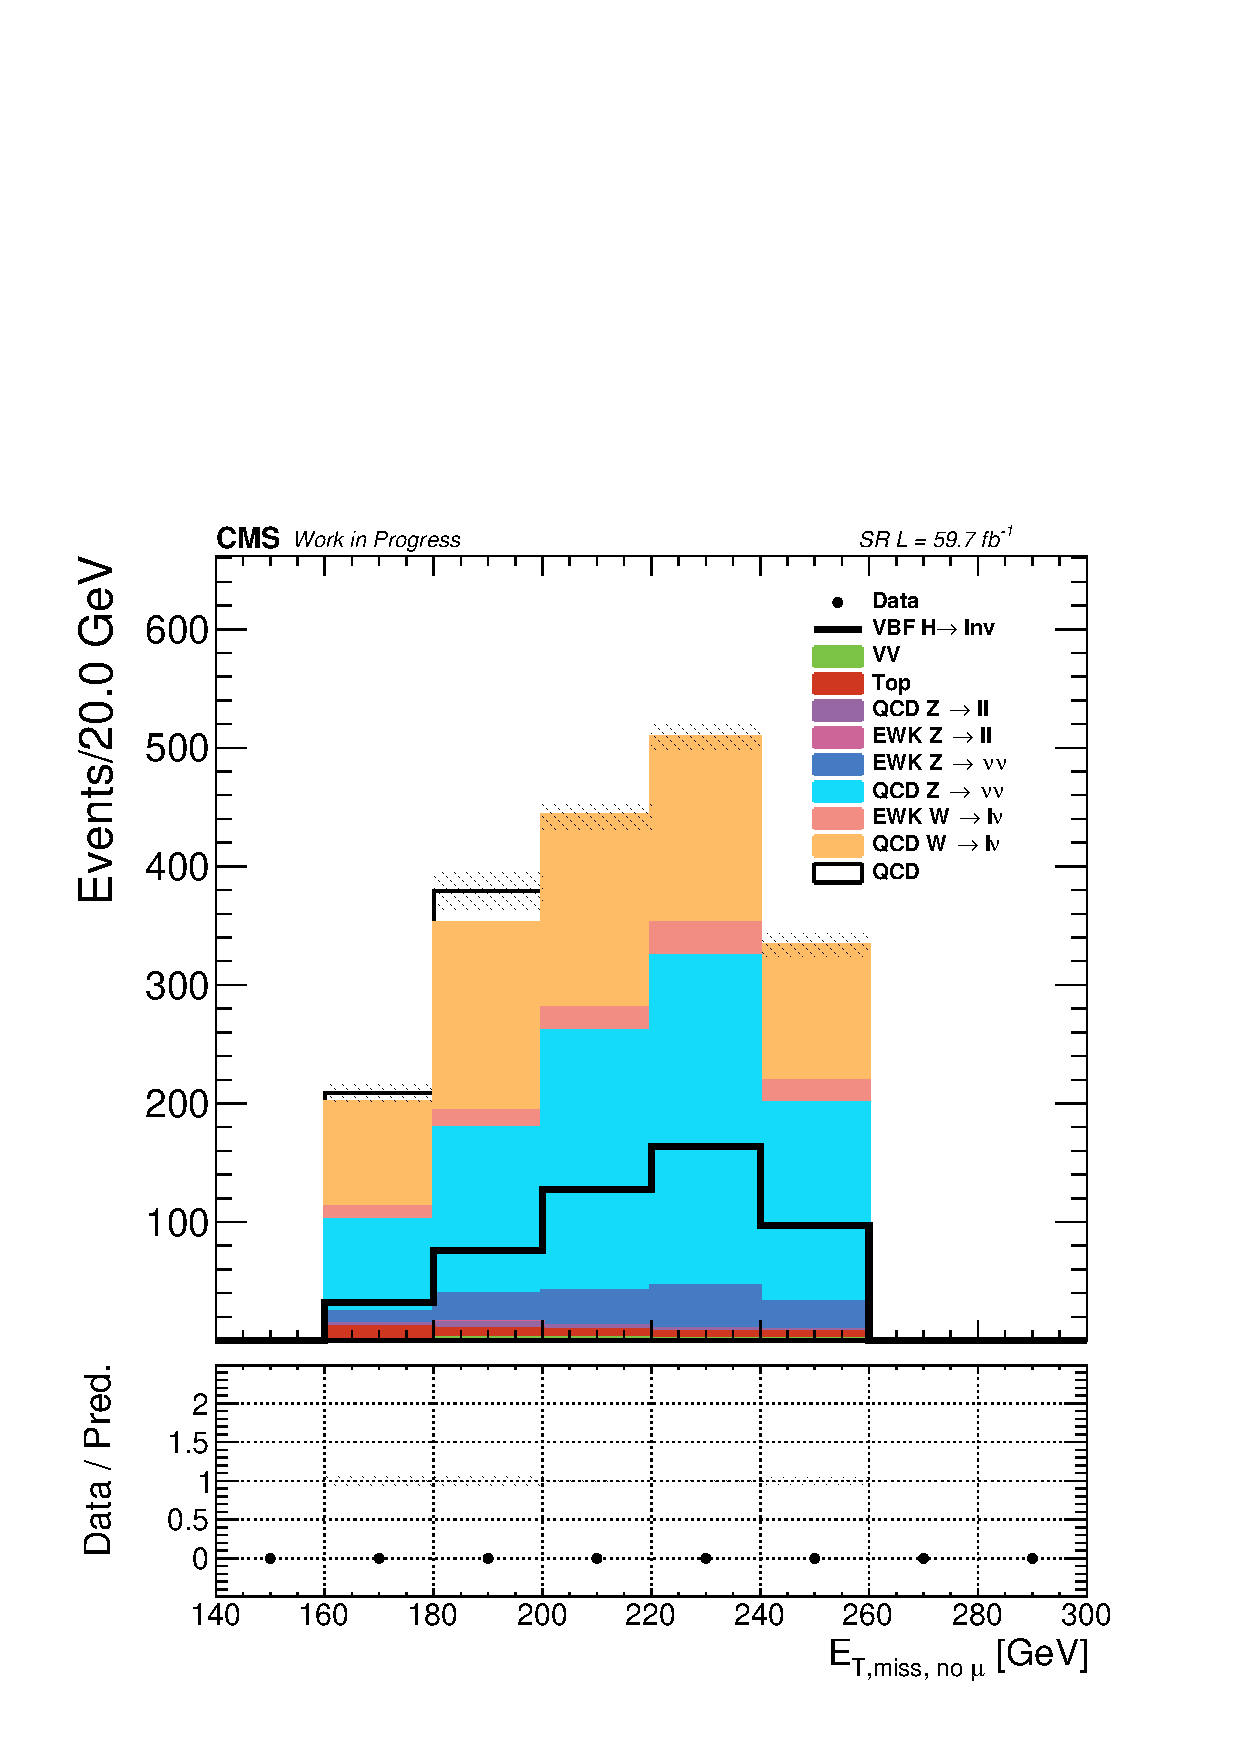
\includegraphics[width=0.49\textwidth]{Analysis_strategy/VTR_2018_SR/MetNoMu.pdf}
    }
    \subfigure[$m_{jj}$]{
    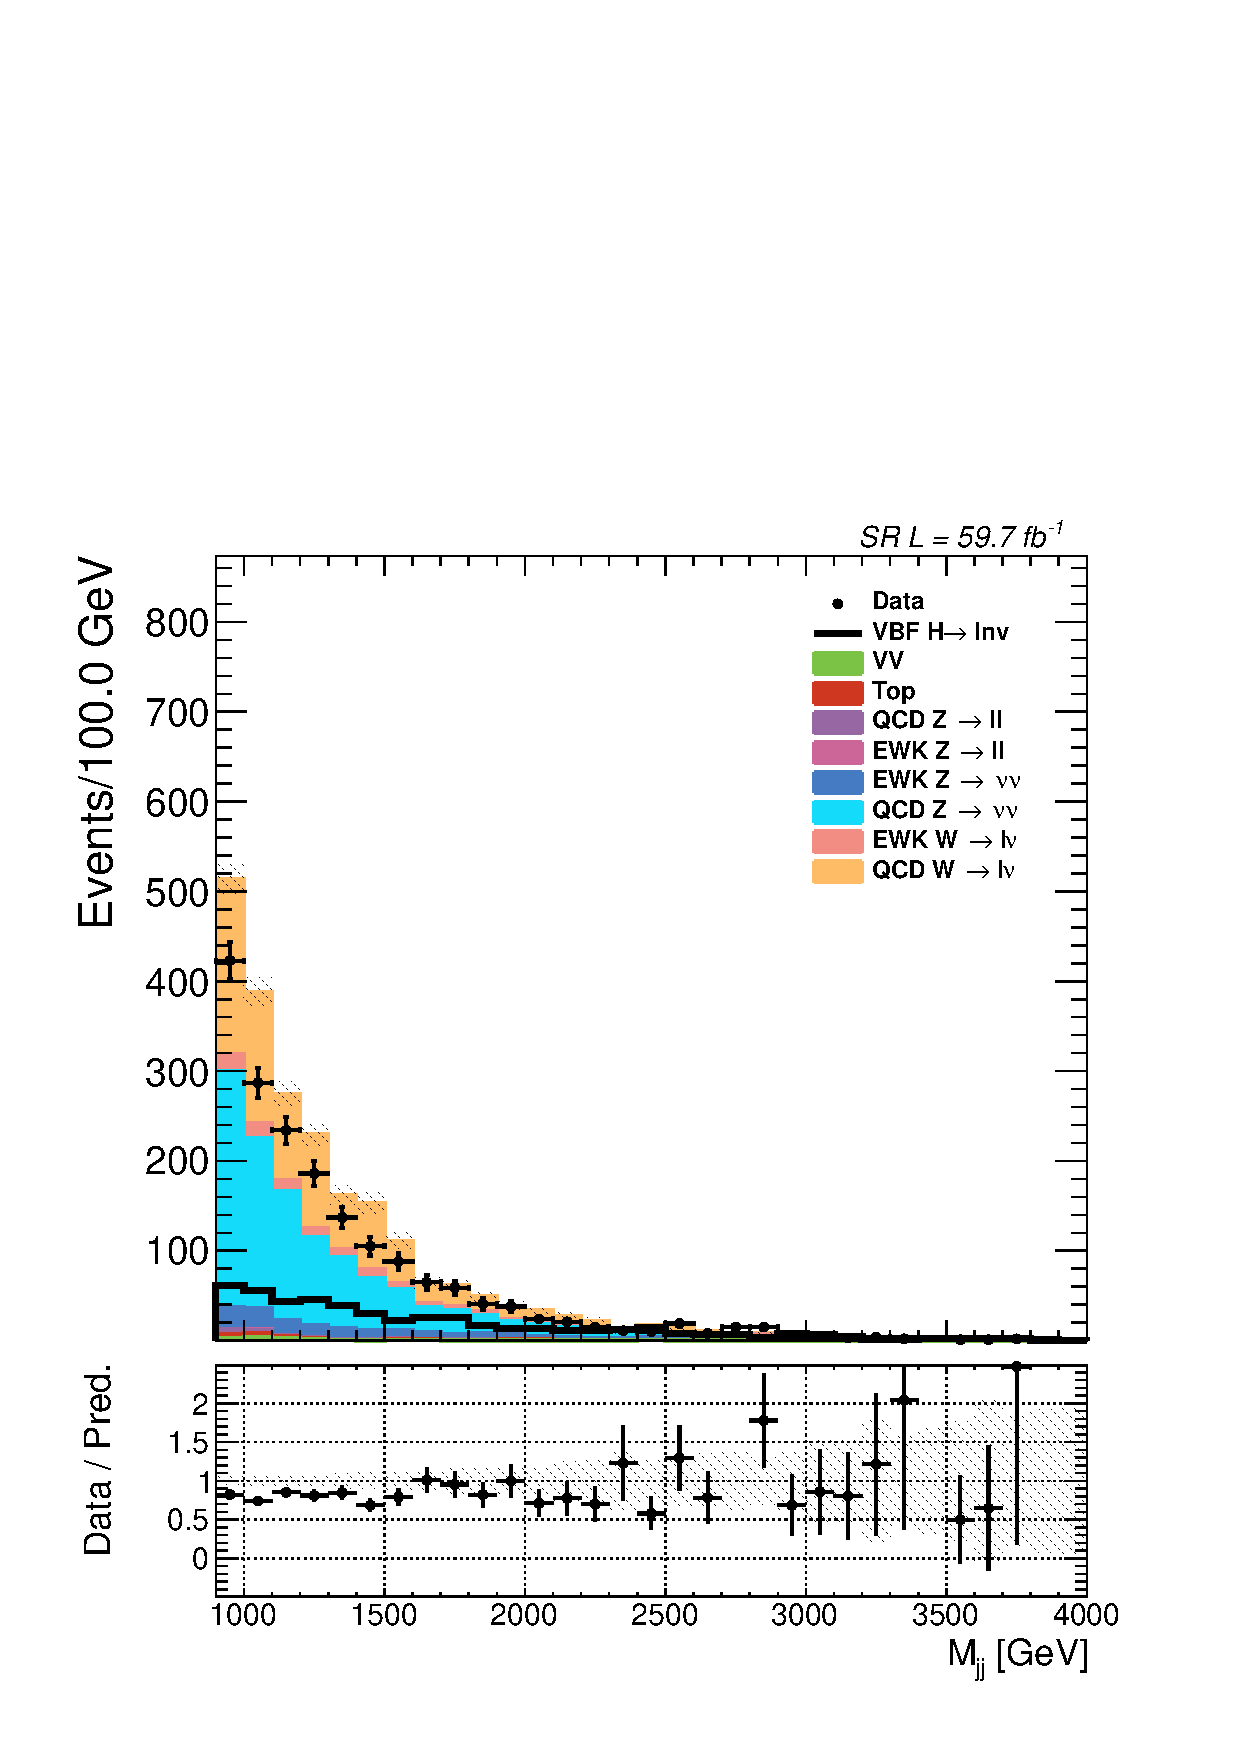
\includegraphics[width=0.49\textwidth]{Analysis_strategy/VTR_2018_SR/lMjj.pdf}}\\
    \subfigure[$\Delta\eta_{jj}$]{
    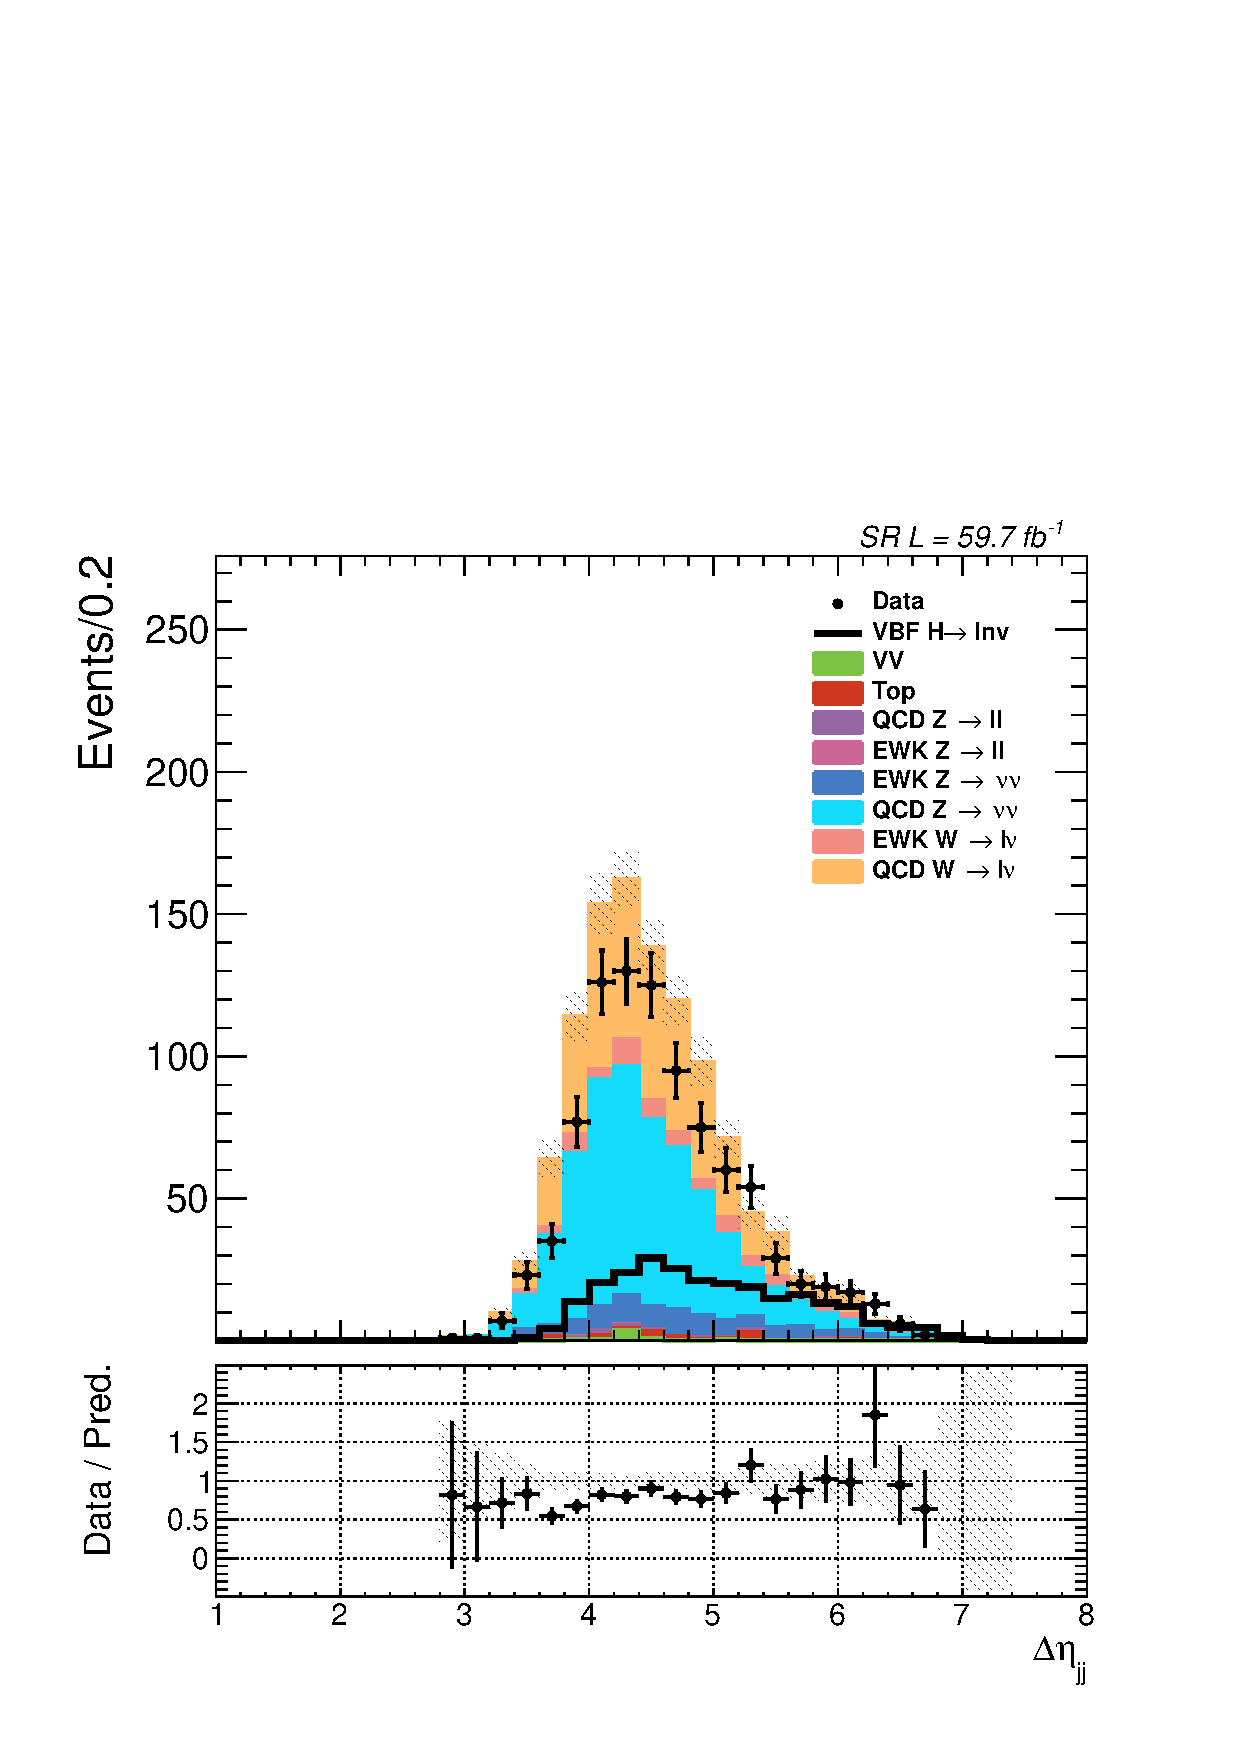
\includegraphics[width=0.49\textwidth]{Analysis_strategy/VTR_2018_SR/lMjj_leading_dEtajj.pdf}
    }
    \subfigure[$\Delta\phi_{jj}$]{
    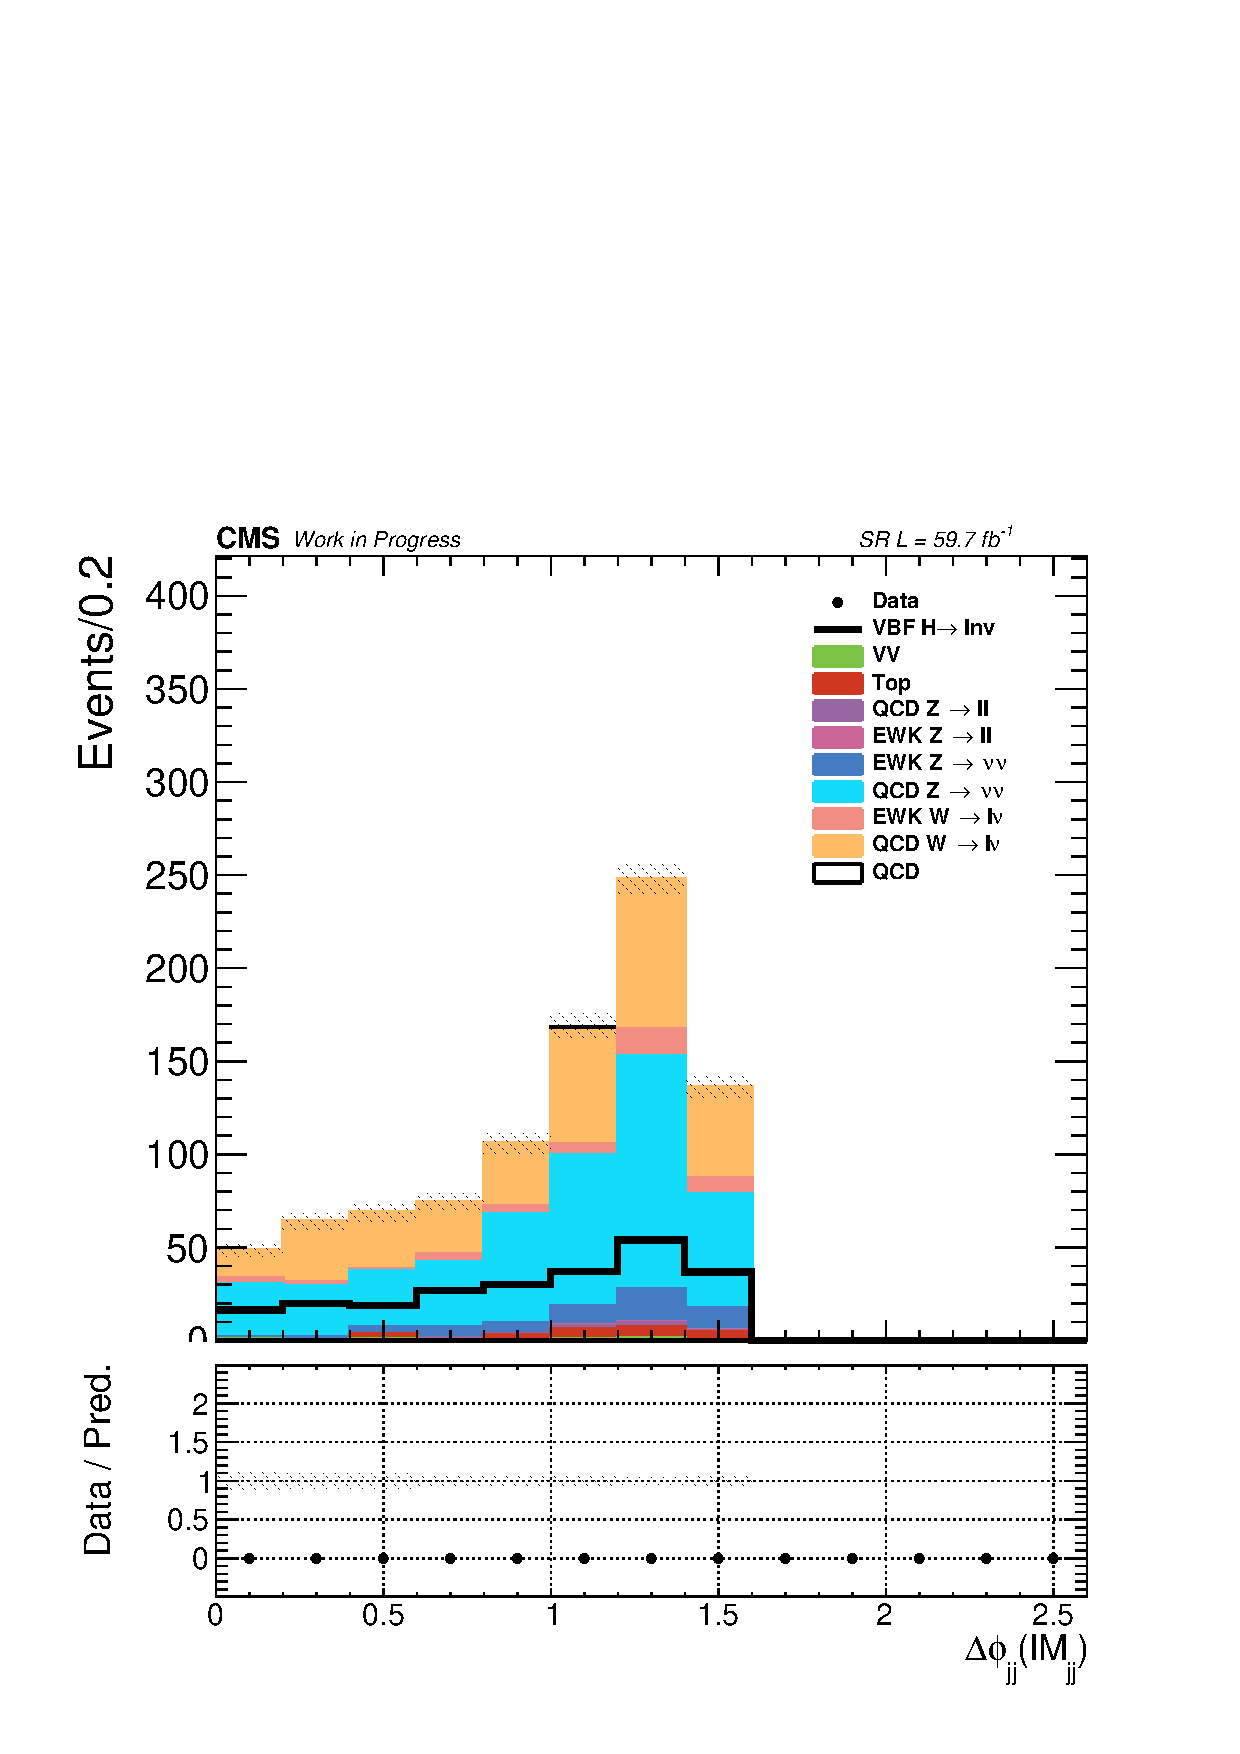
\includegraphics[width=0.49\textwidth]{Analysis_strategy/VTR_2018_SR/lMjj_leading_dPhijj.pdf}
    }
  \caption{Distributions of $E_{T,miss}$, $m_{jj}$, $\Delta\eta_{jj}$ and $\Delta\phi_{jj}$ variables in the SR after the full VTR selection, for 2018 data.}
  \label{fig:2018_VTR_SR_motivation_1}
\end{figure}

\newpage

\hspace{10pt} Figures~\ref{fig:jet_eta_preHornCut_2018} and~\ref{fig:jet_eta_postHornCut_2018} show distributions of jet $\eta$ for the leading jet pair, pre and post mitigation veto being applied, respectively (for both categories).

\begin{figure}[htbp]
  \centering
    \subfigure[$\eta_{j, 1}$ - MTR]{
    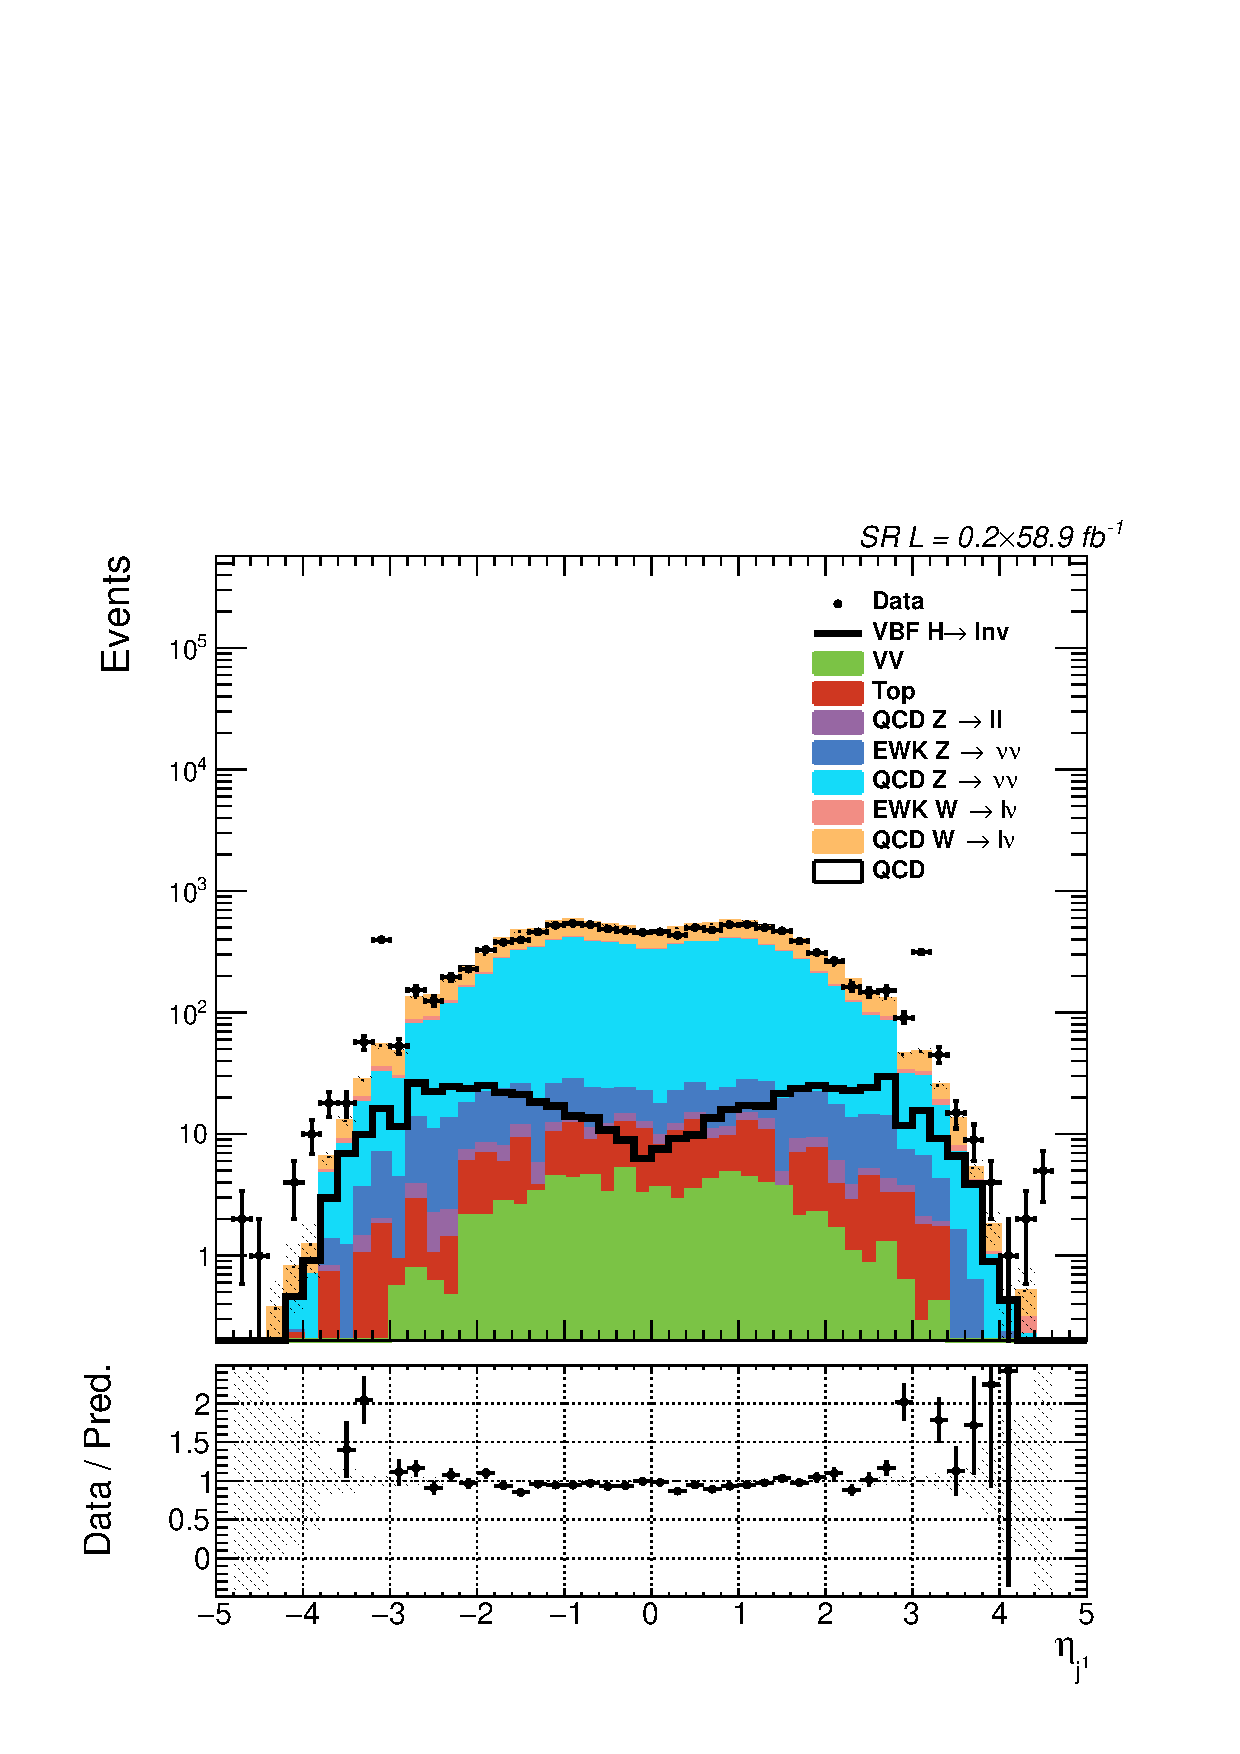
\includegraphics[width=0.47\textwidth]{Analysis_strategy/2018_preHornCut/Leading_jet_eta_log.pdf}
    }
    \subfigure[$\eta_{j, 2}$ - MTR]{
    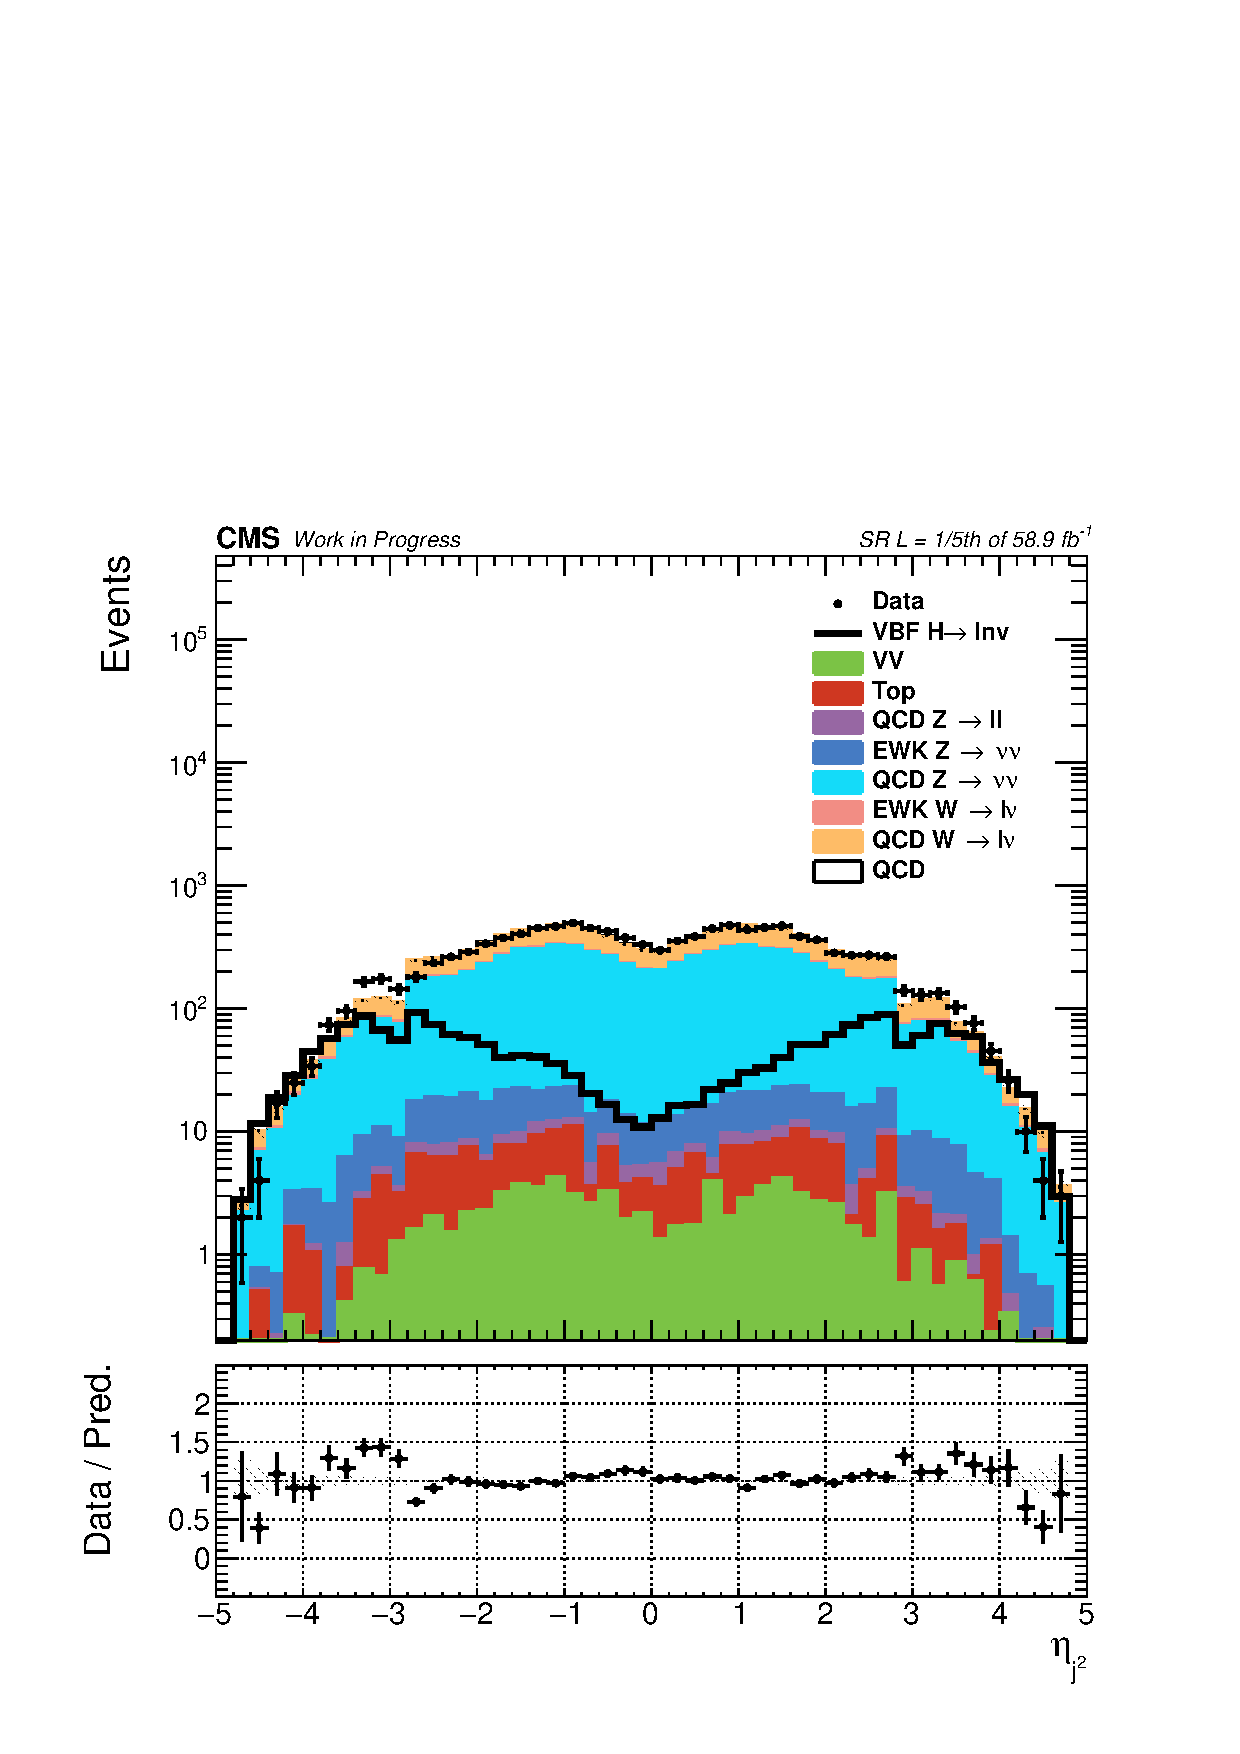
\includegraphics[width=0.47\textwidth]{Analysis_strategy/2018_preHornCut/Subleading_jet_eta_log.pdf}
    }\\
    \subfigure[$\eta_{j, 1}$ - VTR]{
    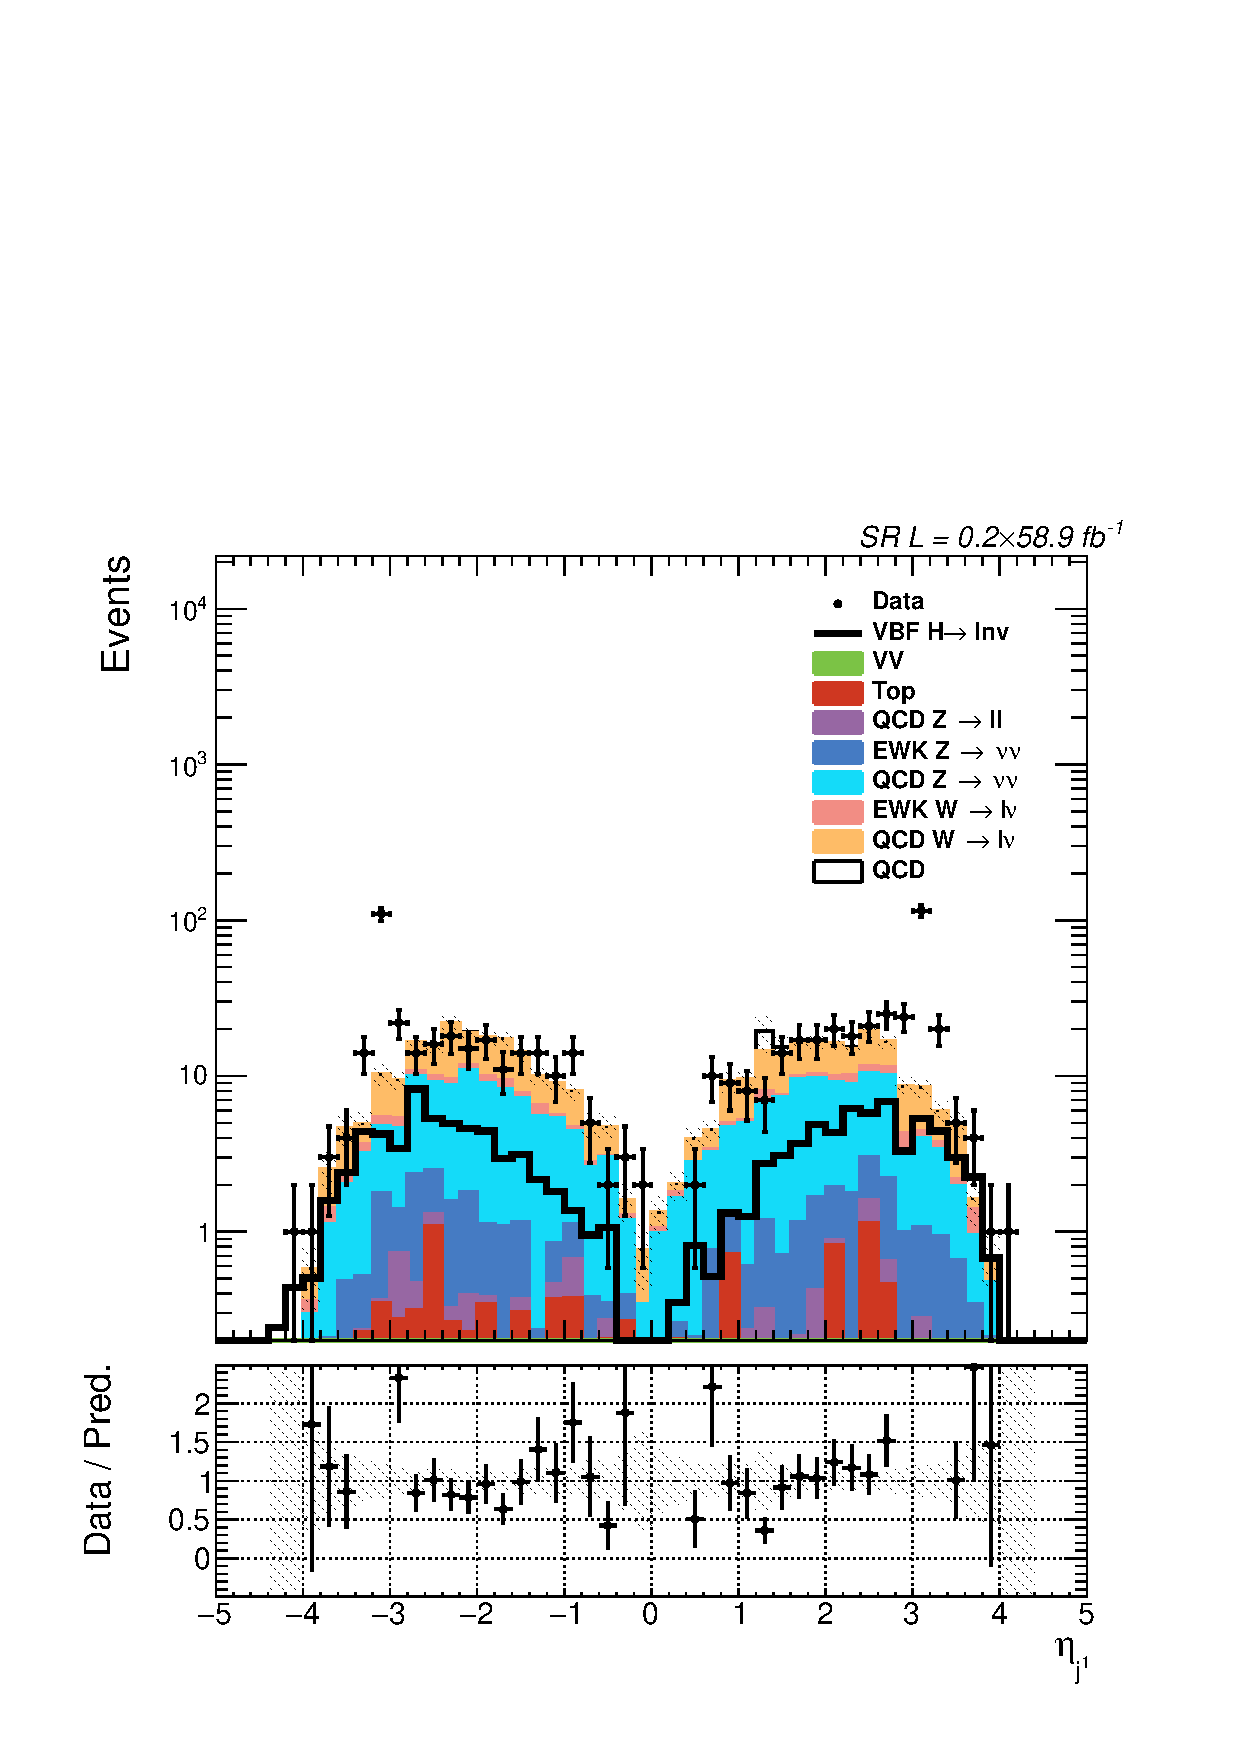
\includegraphics[width=0.47\textwidth]{Analysis_strategy/2018_preHornCut/VTRLeading_jet_eta_log.pdf}
    }
    \subfigure[$\eta_{j, 2}$ - VTR]{
    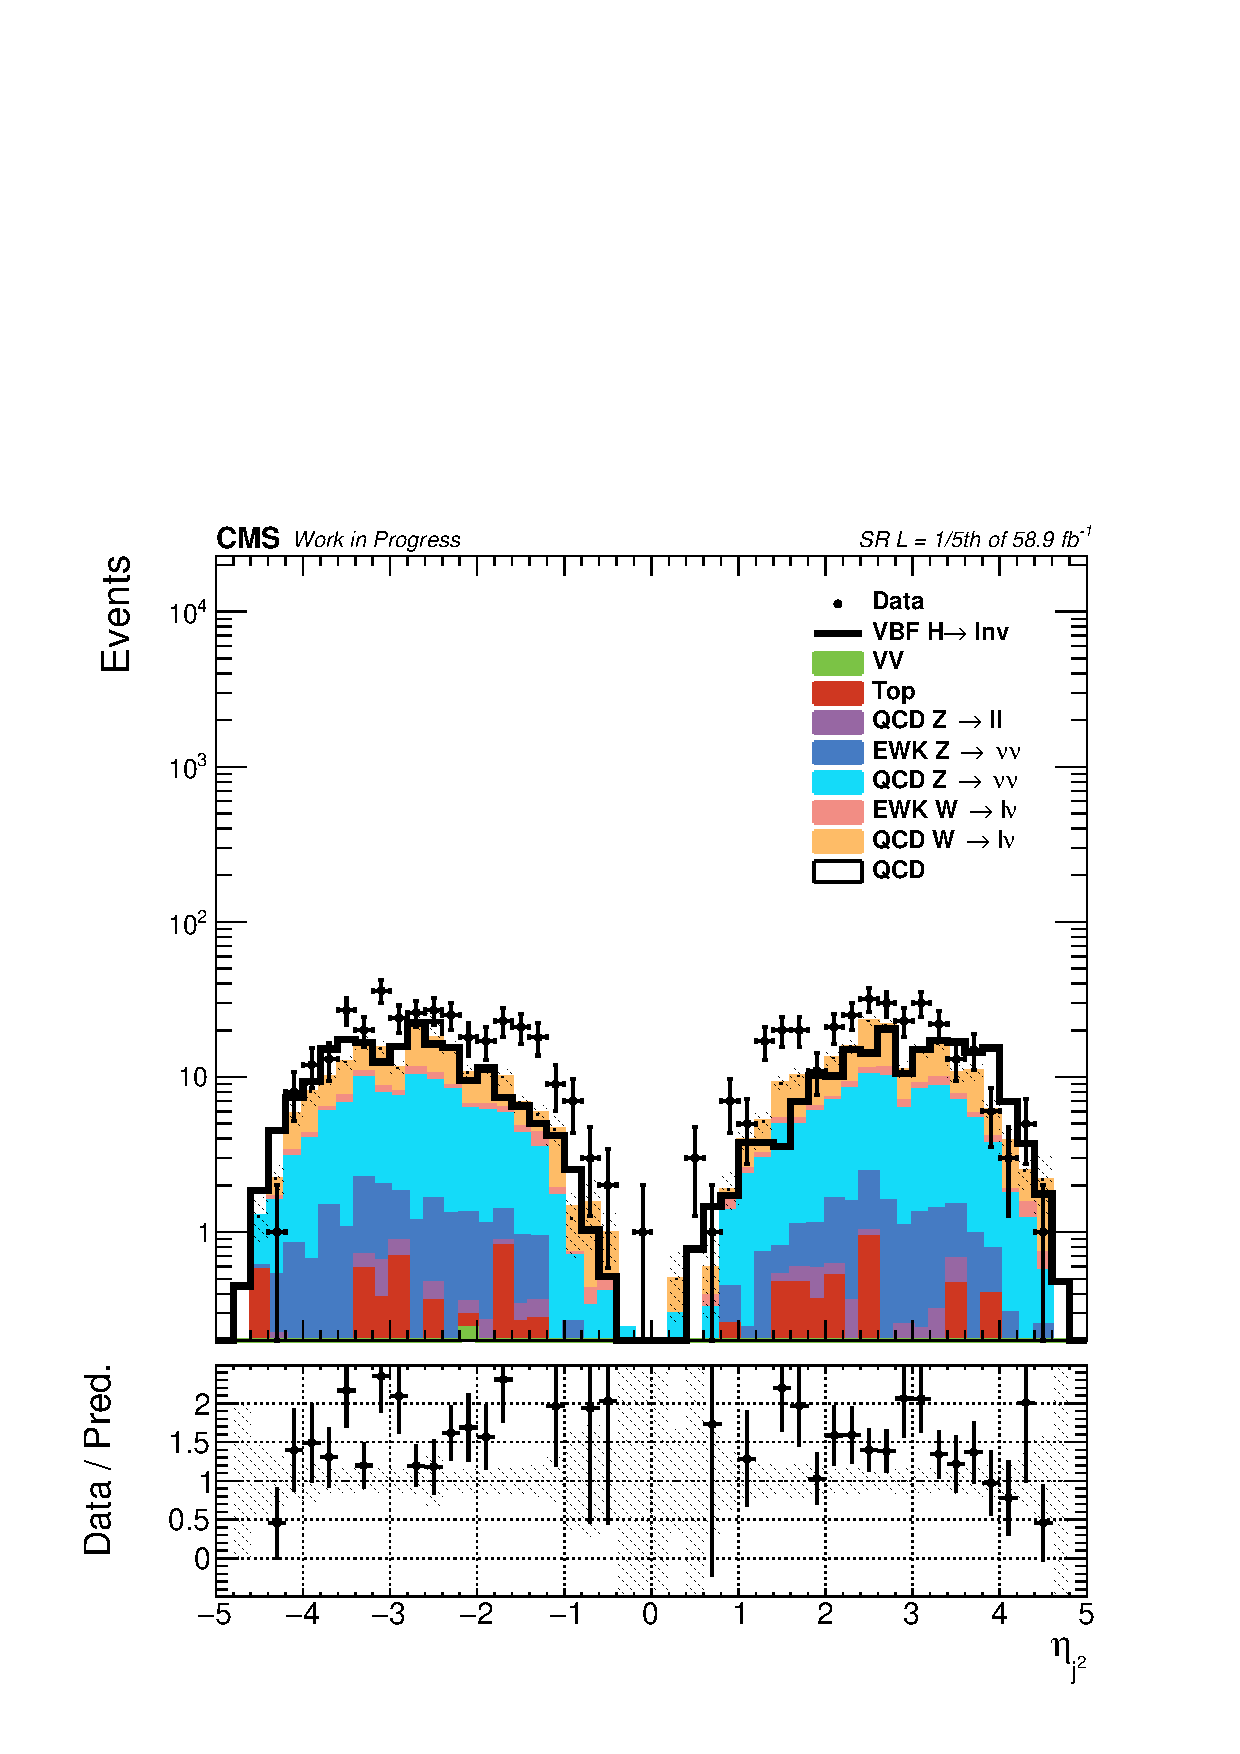
\includegraphics[width=0.47\textwidth]{Analysis_strategy/2018_preHornCut/VTRSubleading_jet_eta_log.pdf}
    }
  \caption{Distributions of $\eta_{j, 1}$ (left) and $\eta_{j, 2}$ (right) variables in the signal region after the unbinding of 1/5th of the 2018 data. Both MTR (top) and VTR (bottom) categories are presented.}
  \label{fig:jet_eta_preHornCut_2018}
\end{figure}

\begin{figure}[htbp]
  \centering
    \subfigure[$\eta_{j, 1}$ - MTR]{
    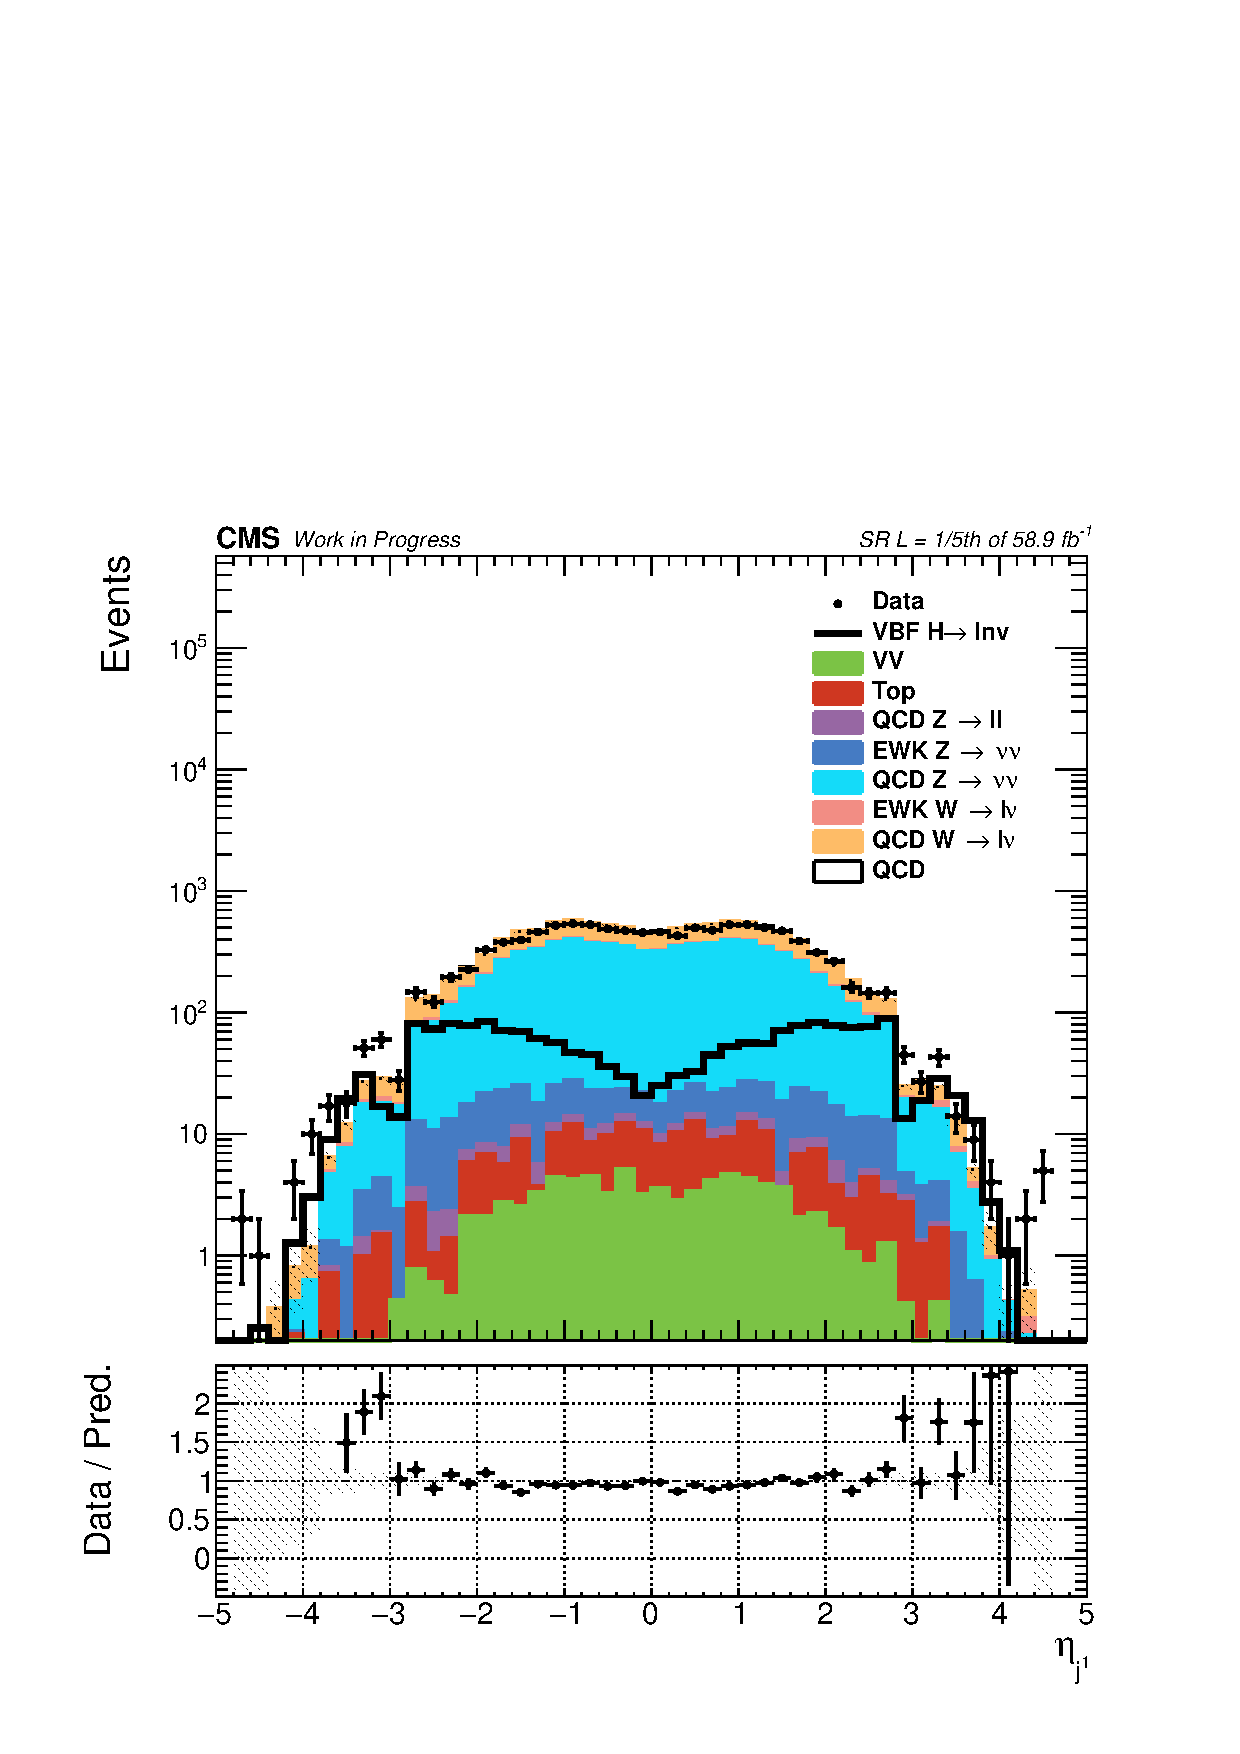
\includegraphics[width=0.49\textwidth]{Analysis_strategy/2018_postHornCut/Leading_jet_eta_log.pdf}
    }
    \subfigure[$\eta_{j, 2}$ - MTR]{
    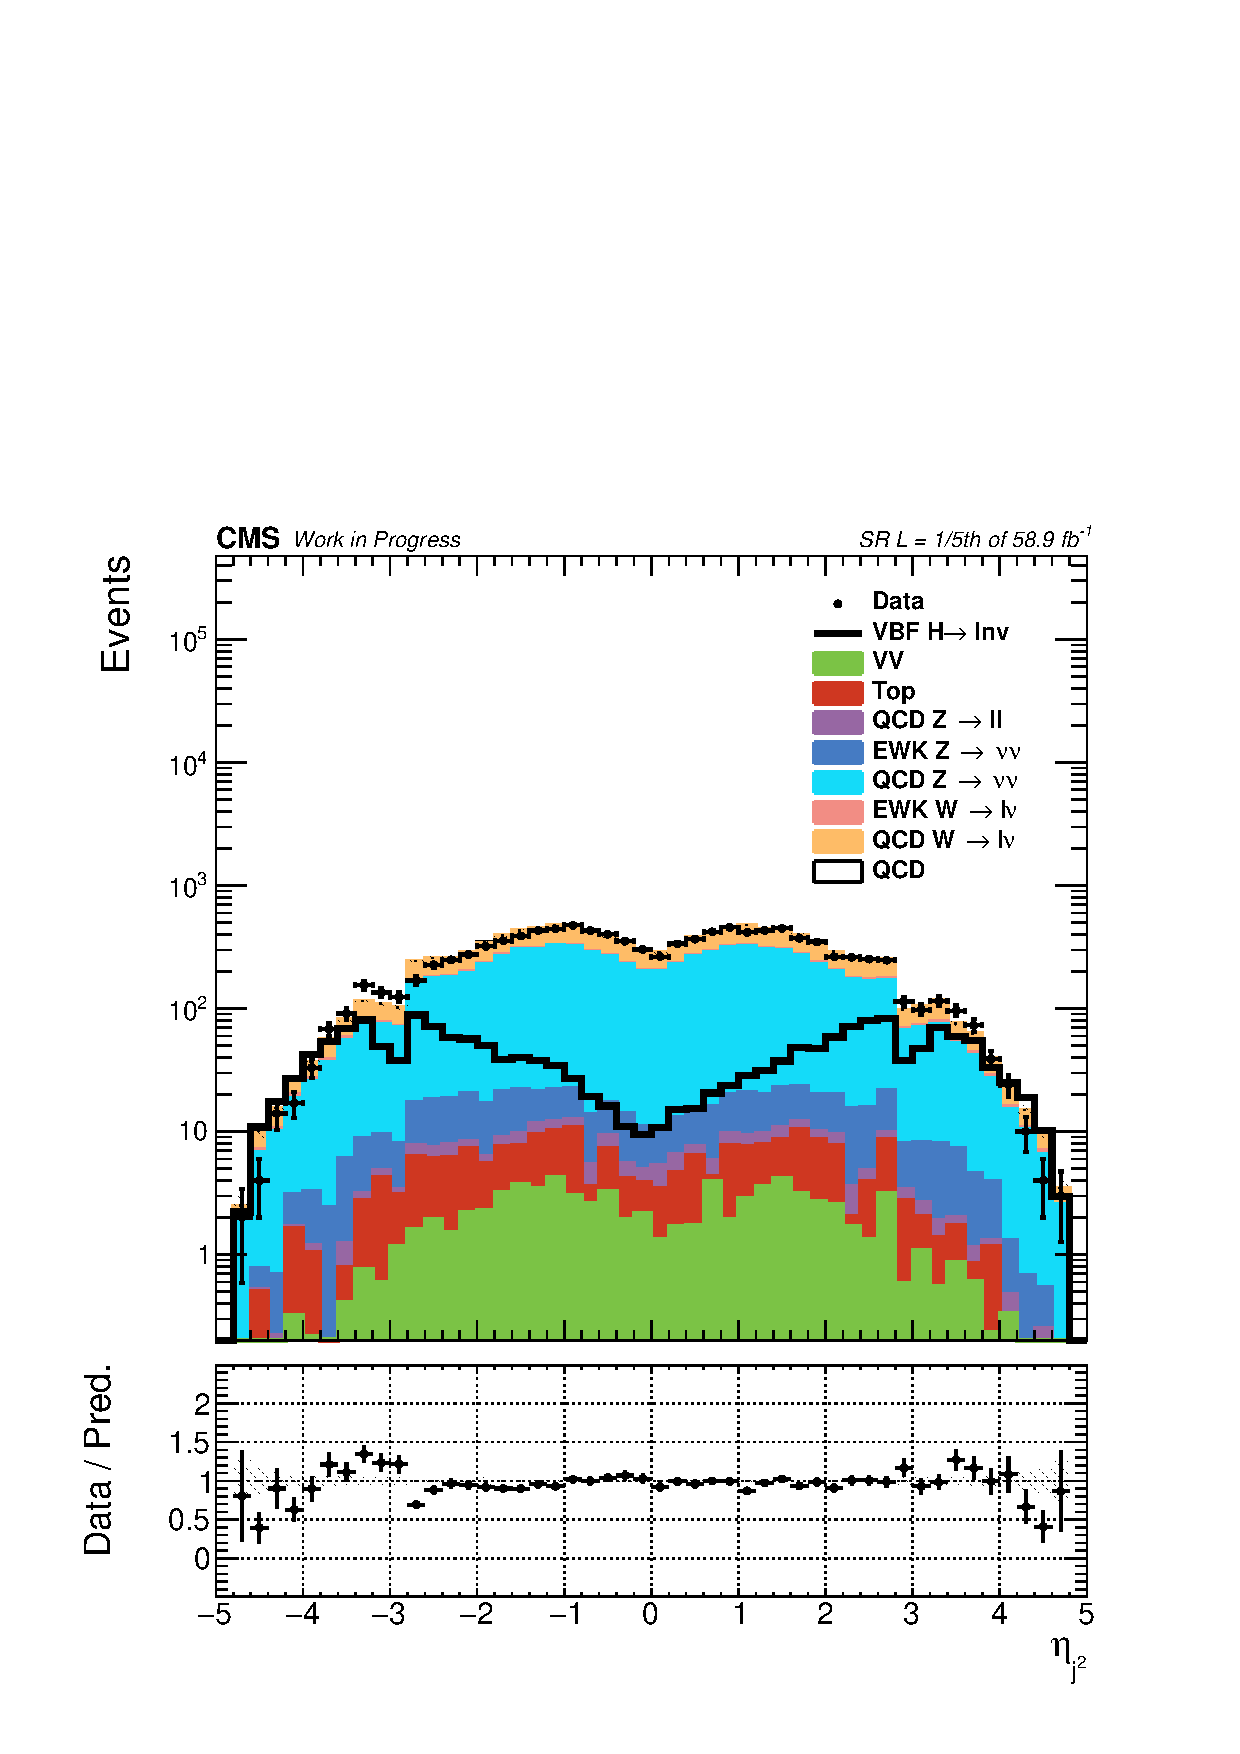
\includegraphics[width=0.49\textwidth]{Analysis_strategy/2018_postHornCut/Subleading_jet_eta_log.pdf}
    }\\
    \subfigure[$\eta_{j, 1}$ - VTR]{
    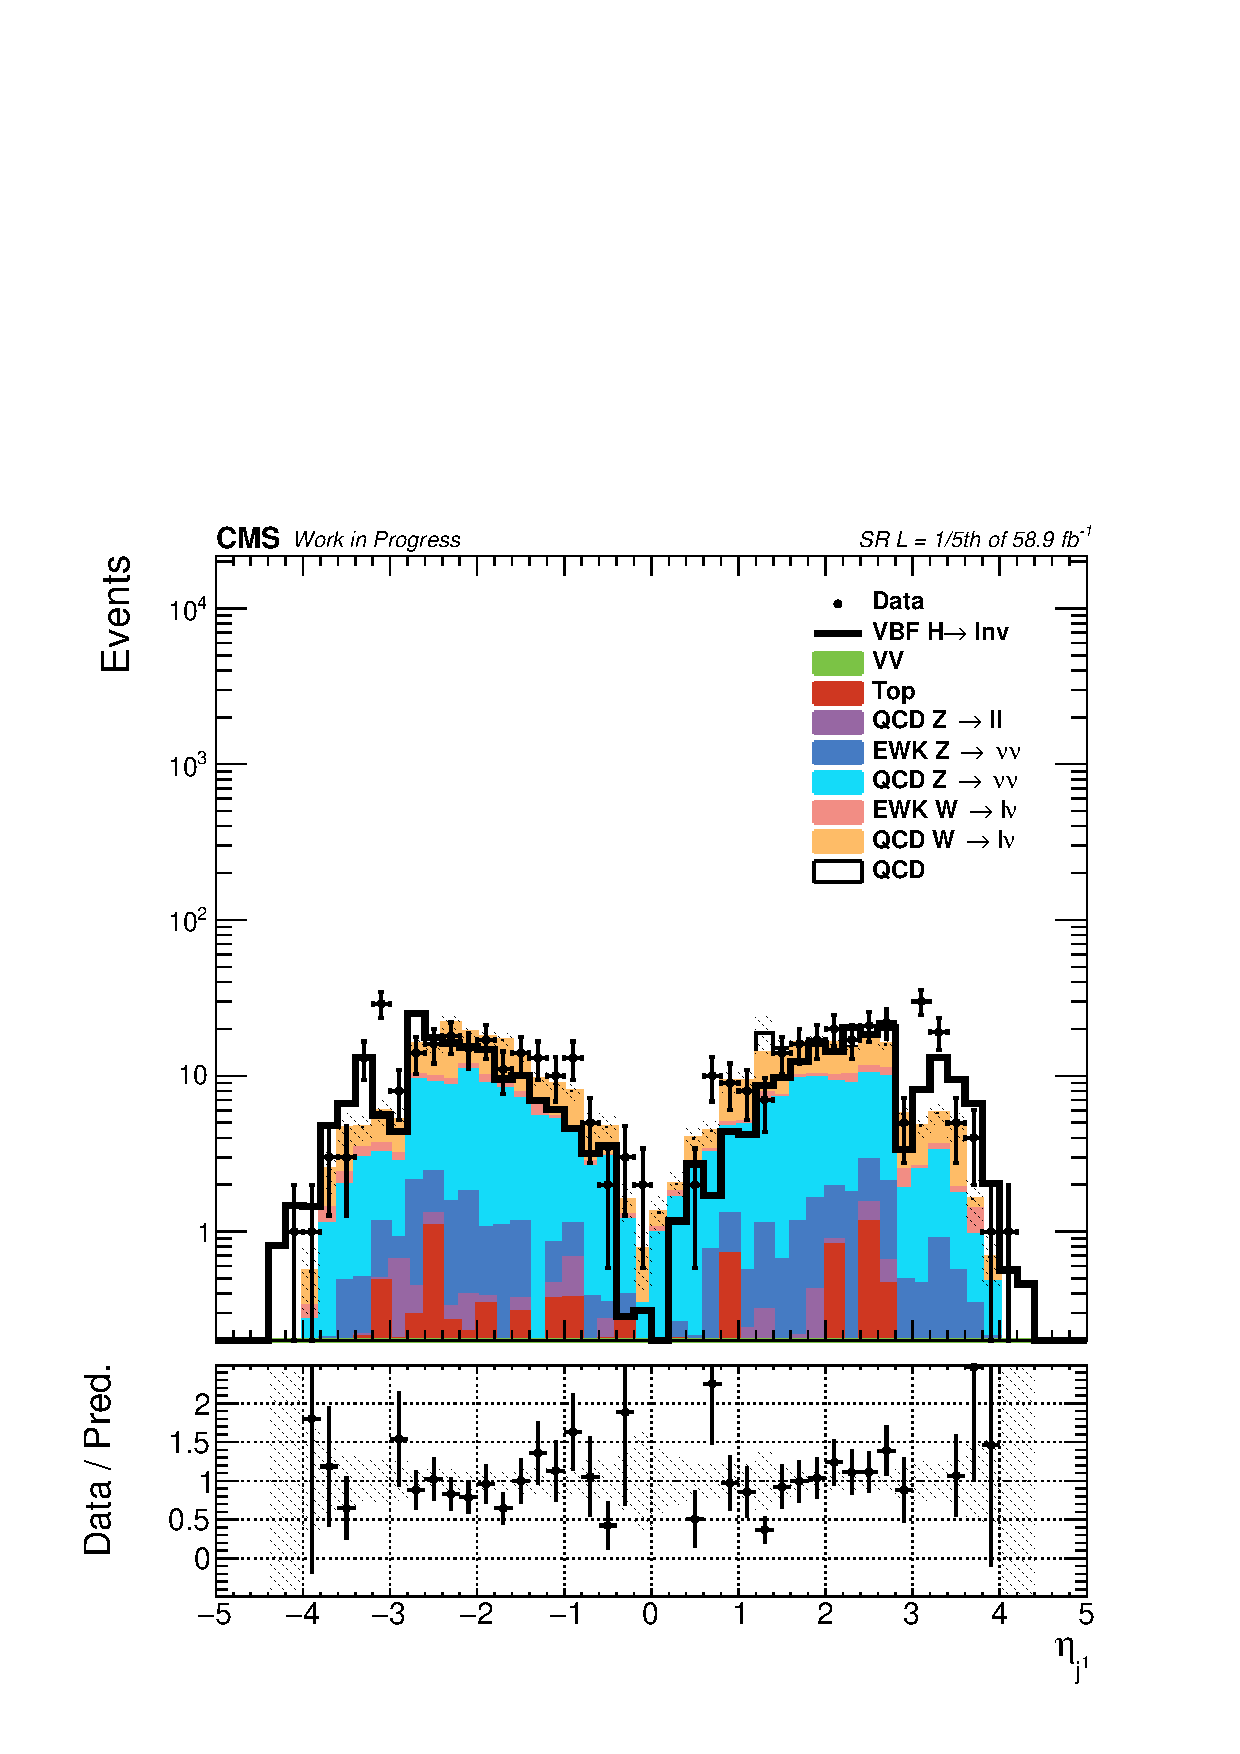
\includegraphics[width=0.49\textwidth]{Analysis_strategy/2018_postHornCut/VTRLeading_jet_eta_log.pdf}
    }
    \subfigure[$\eta_{j, 2}$ - VTR]{
    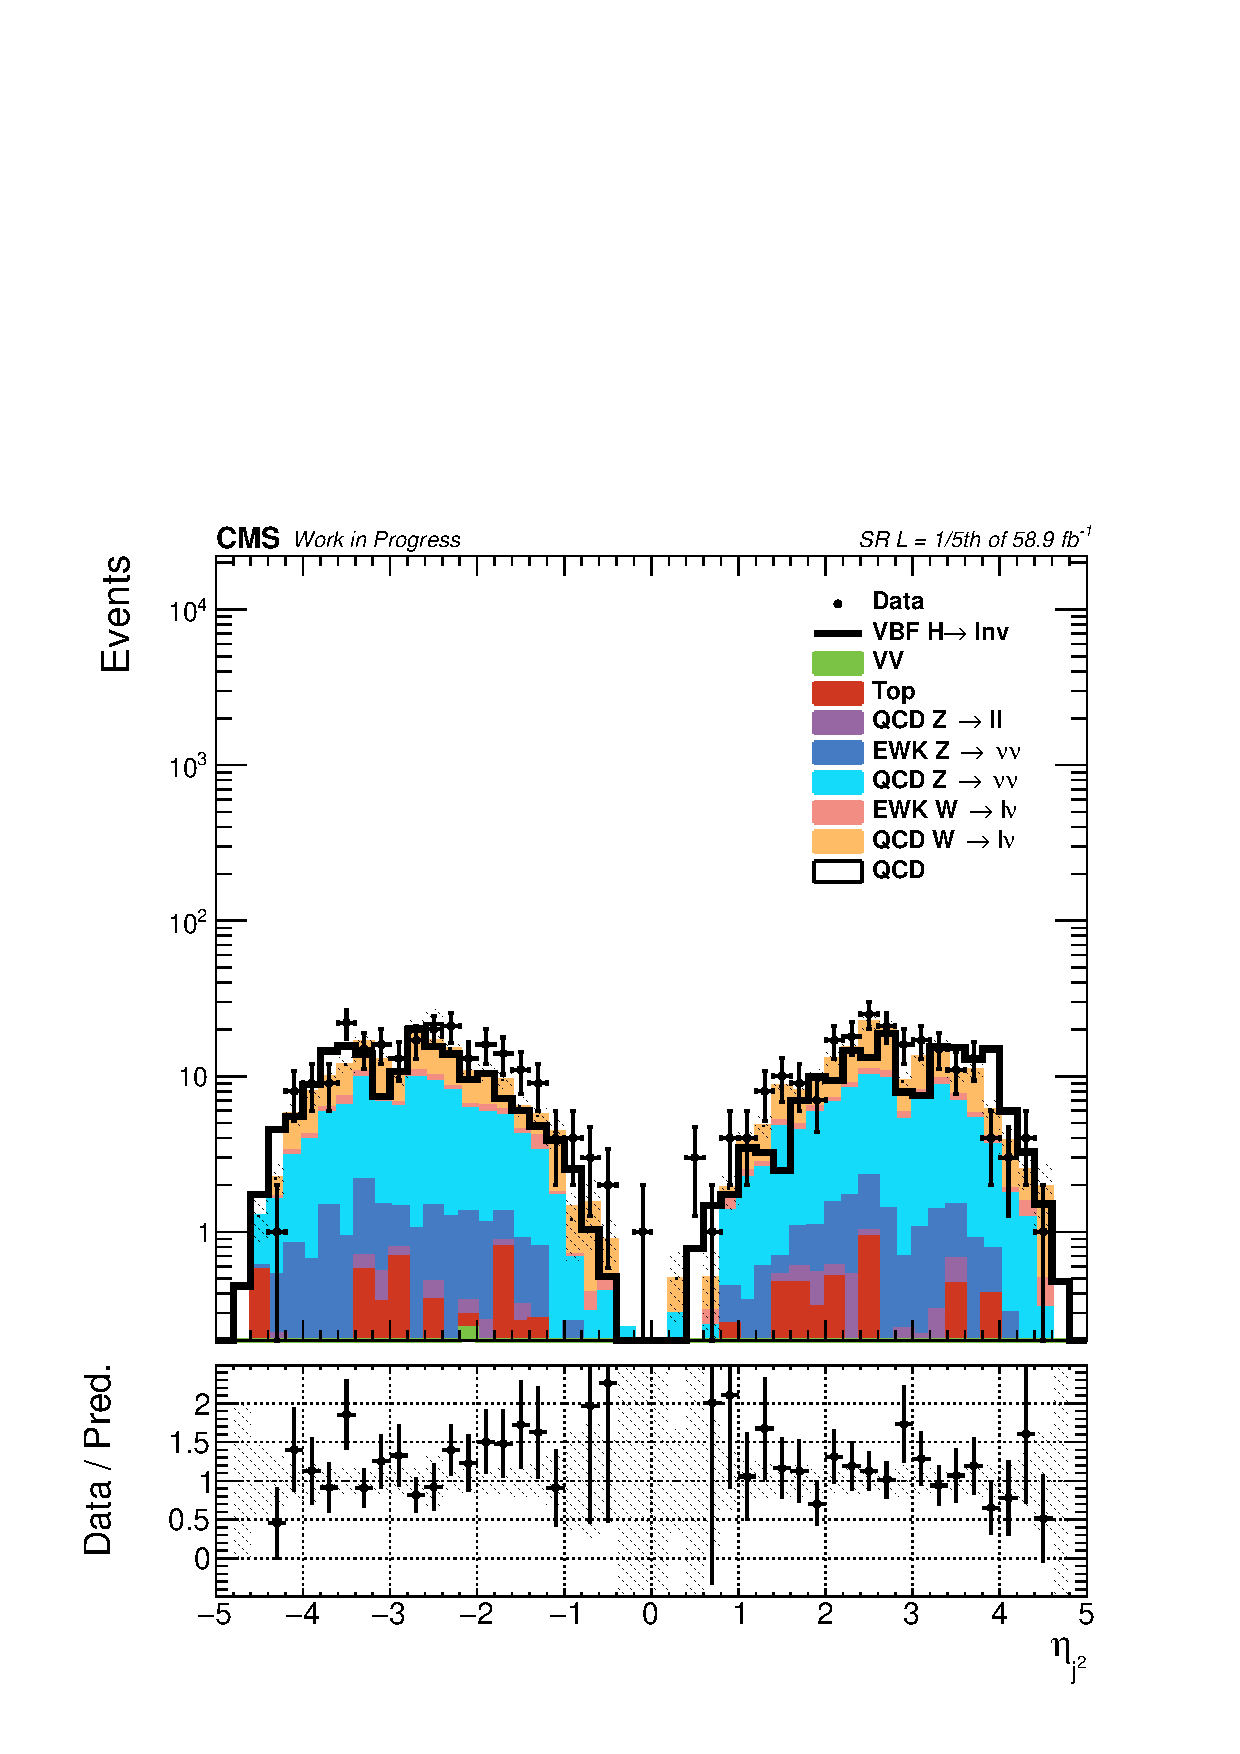
\includegraphics[width=0.49\textwidth]{Analysis_strategy/2018_postHornCut/VTRSubleading_jet_eta_log.pdf}
    }
  \caption{Distributions of $\eta_{j, 1}$ (left) and $\eta_{j, 2}$ (right) variables in the signal region after the unbinding of 1/5th of the 2018 data and the mitigation of the jet "horns" effect. Both MTR (top) and VTR (bottom) categories are presented.}
  \label{fig:jet_eta_postHornCut_2018}
\end{figure}

\newpage



\section{Dedicated CRs - supplementary material}
\label{app:CRs}.

\begin{figure}[htbp]
  \centering
    \subfigure[$\phi_{E_{T,miss}^{no,l}}$ - MTR]{
    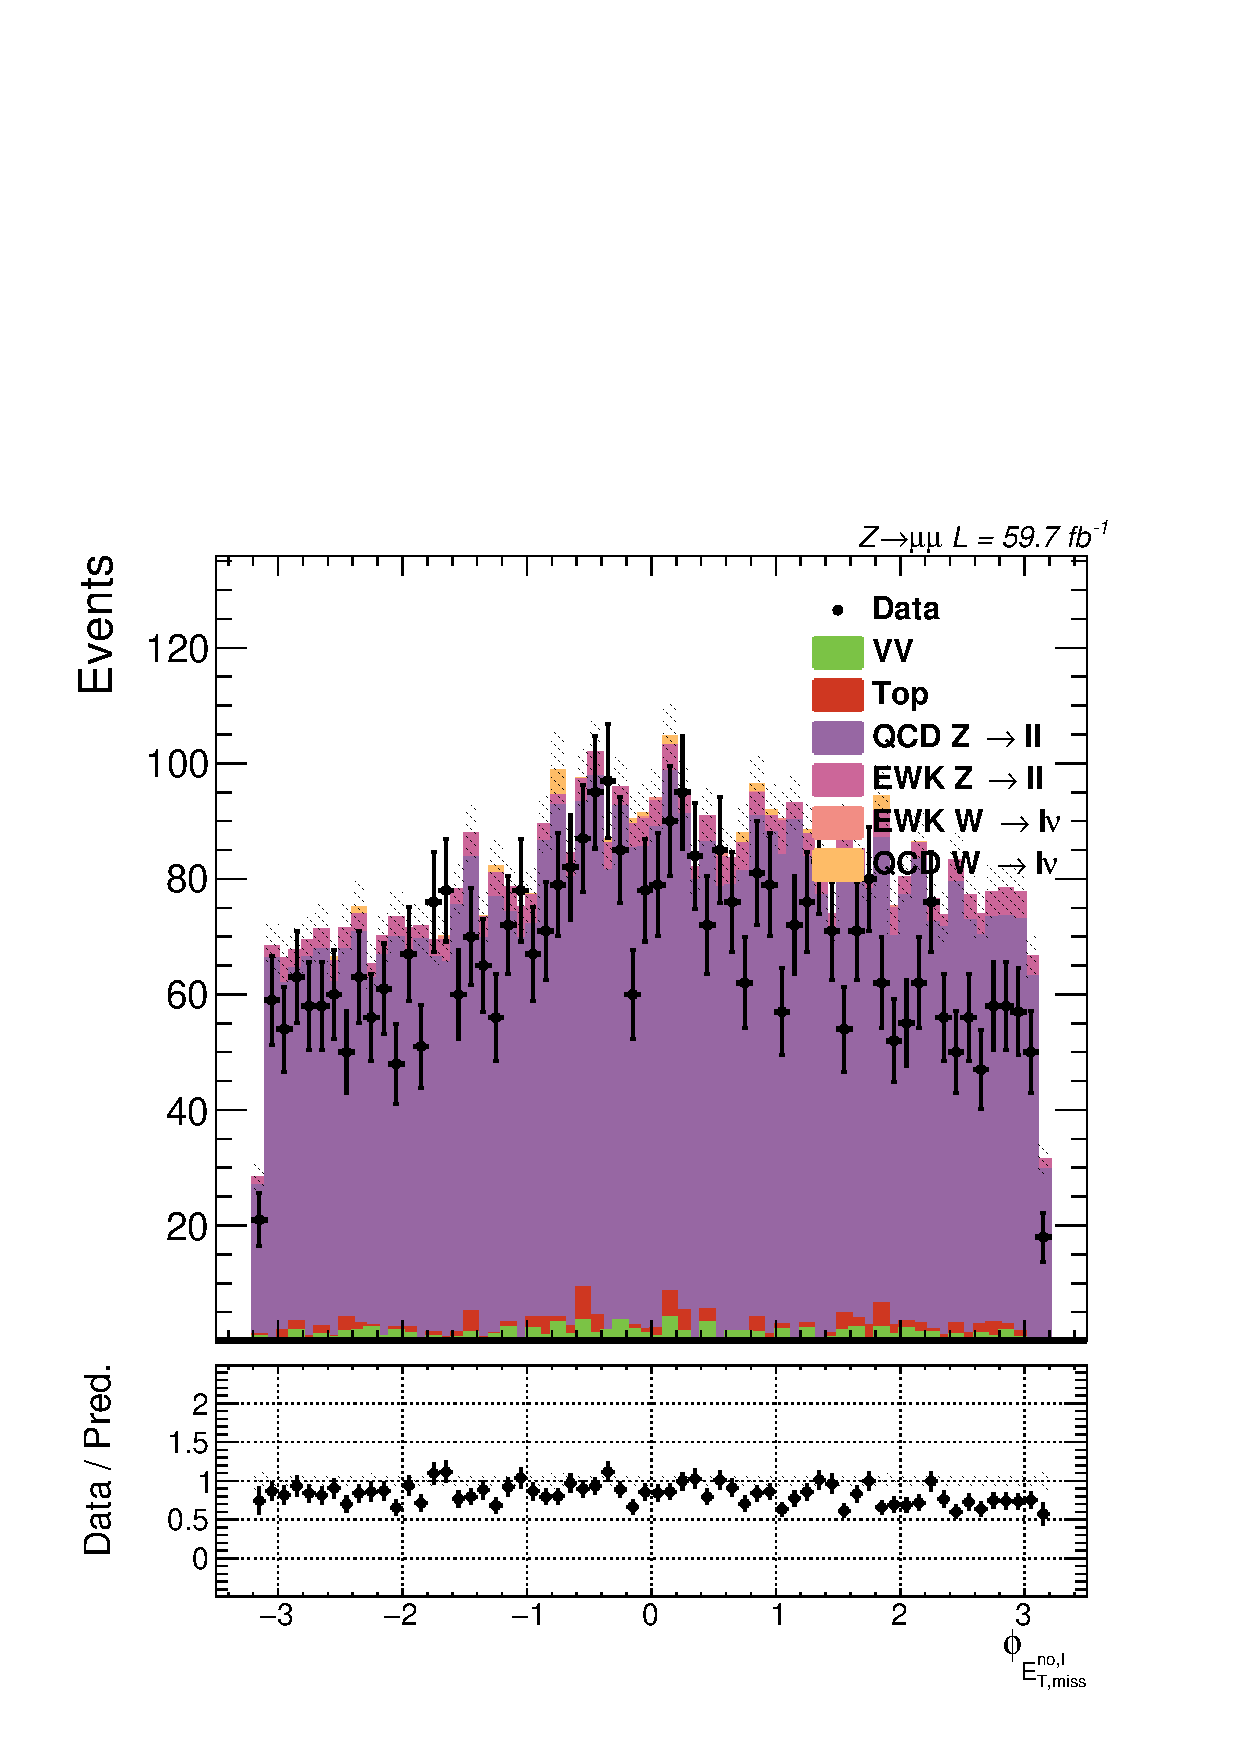
\includegraphics[width=0.47\textwidth]{Control_Regions/Zmumu_noHEM/MetNoMu_phi.pdf}
    }\\
    \subfigure[$\phi_{j1}$ - MTR]{
    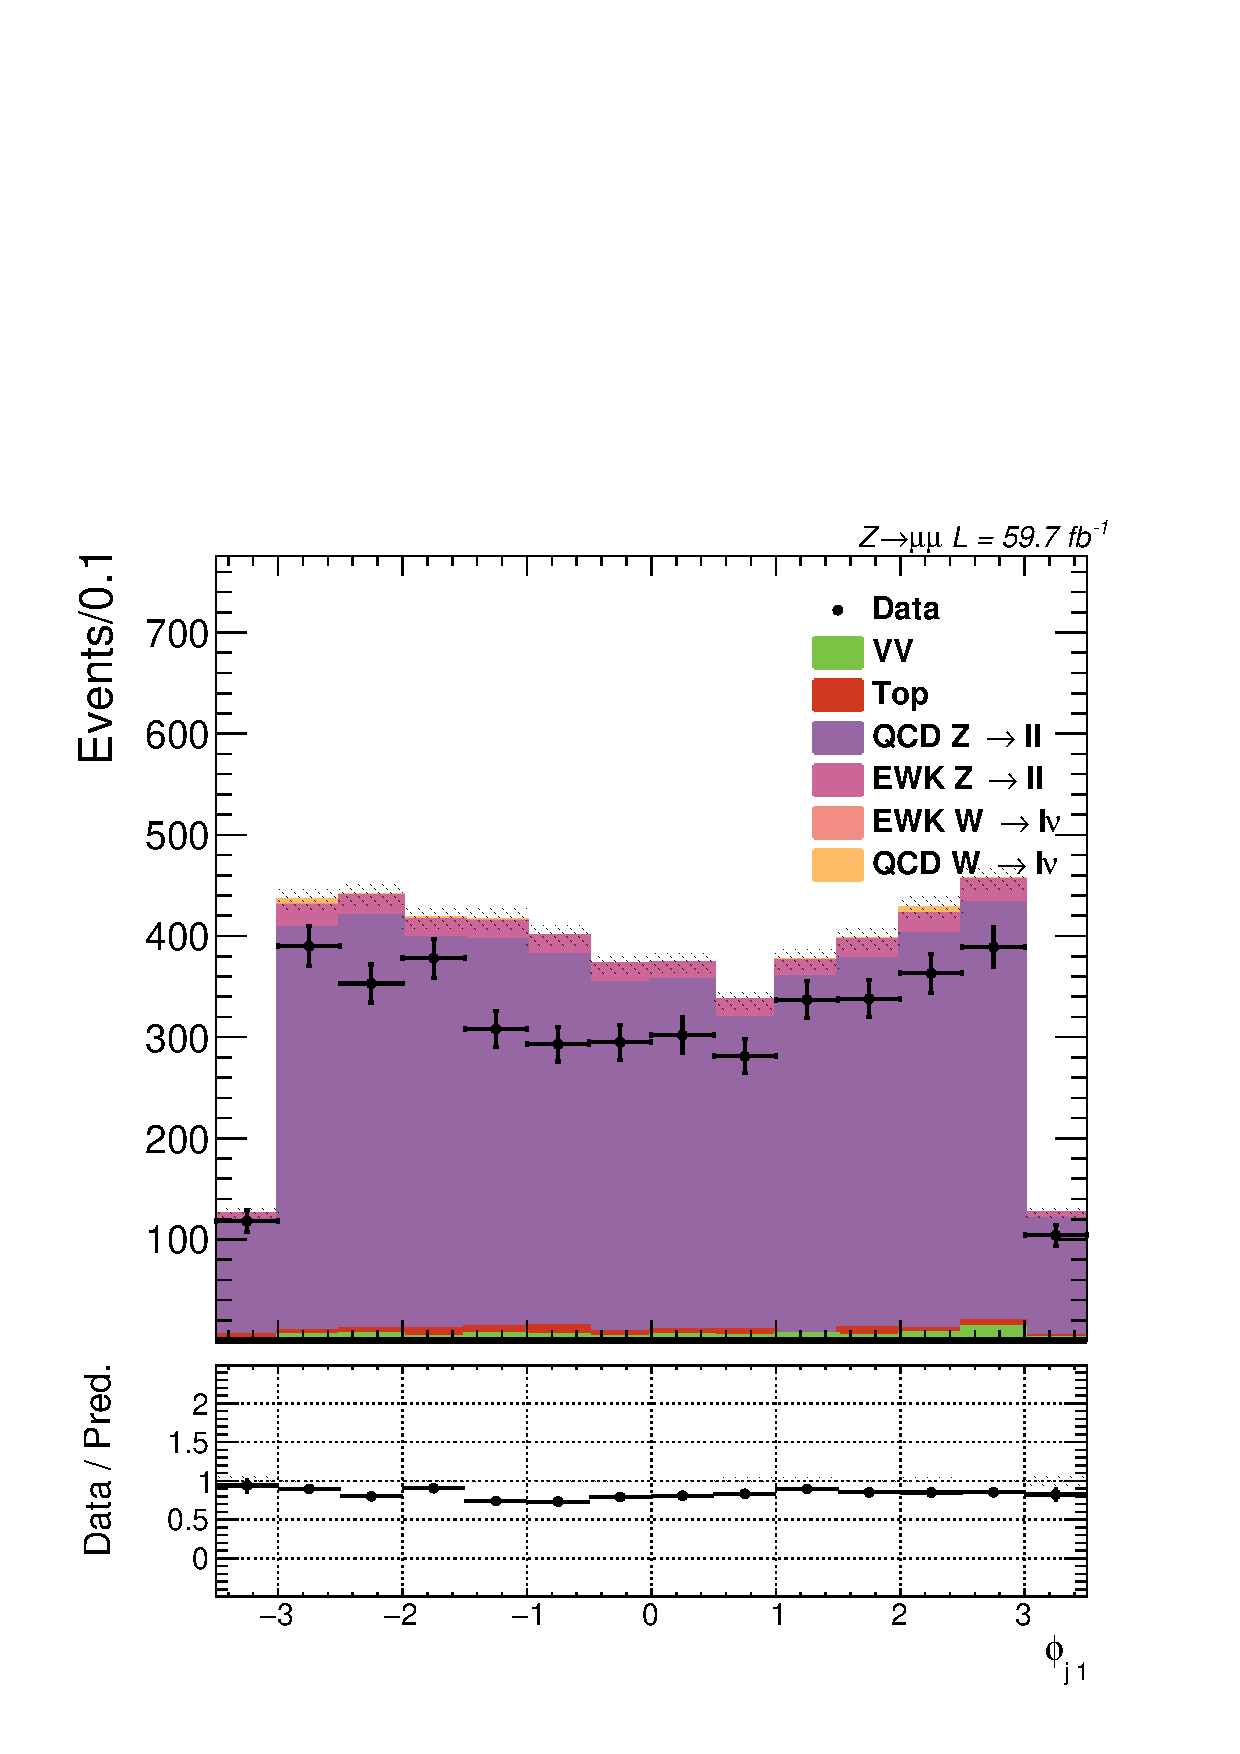
\includegraphics[width=0.47\textwidth]{Control_Regions/Zmumu_noHEM/Leading_jet_phi.pdf}
    }
  \caption{Distributions of $\phi_{E_{T,miss}^{no,l}}$ (a) and $\phi_{j1}$ (b) variables in the double muon CR for the MTR 2018 category, showing the absence of effects related to the HEM problem. }
  \label{app:Zmumu_noHEM}
\end{figure}


\begin{figure}[htbp]
  \centering
    \subfigure[$E_{T,miss}$ - MTR]{
    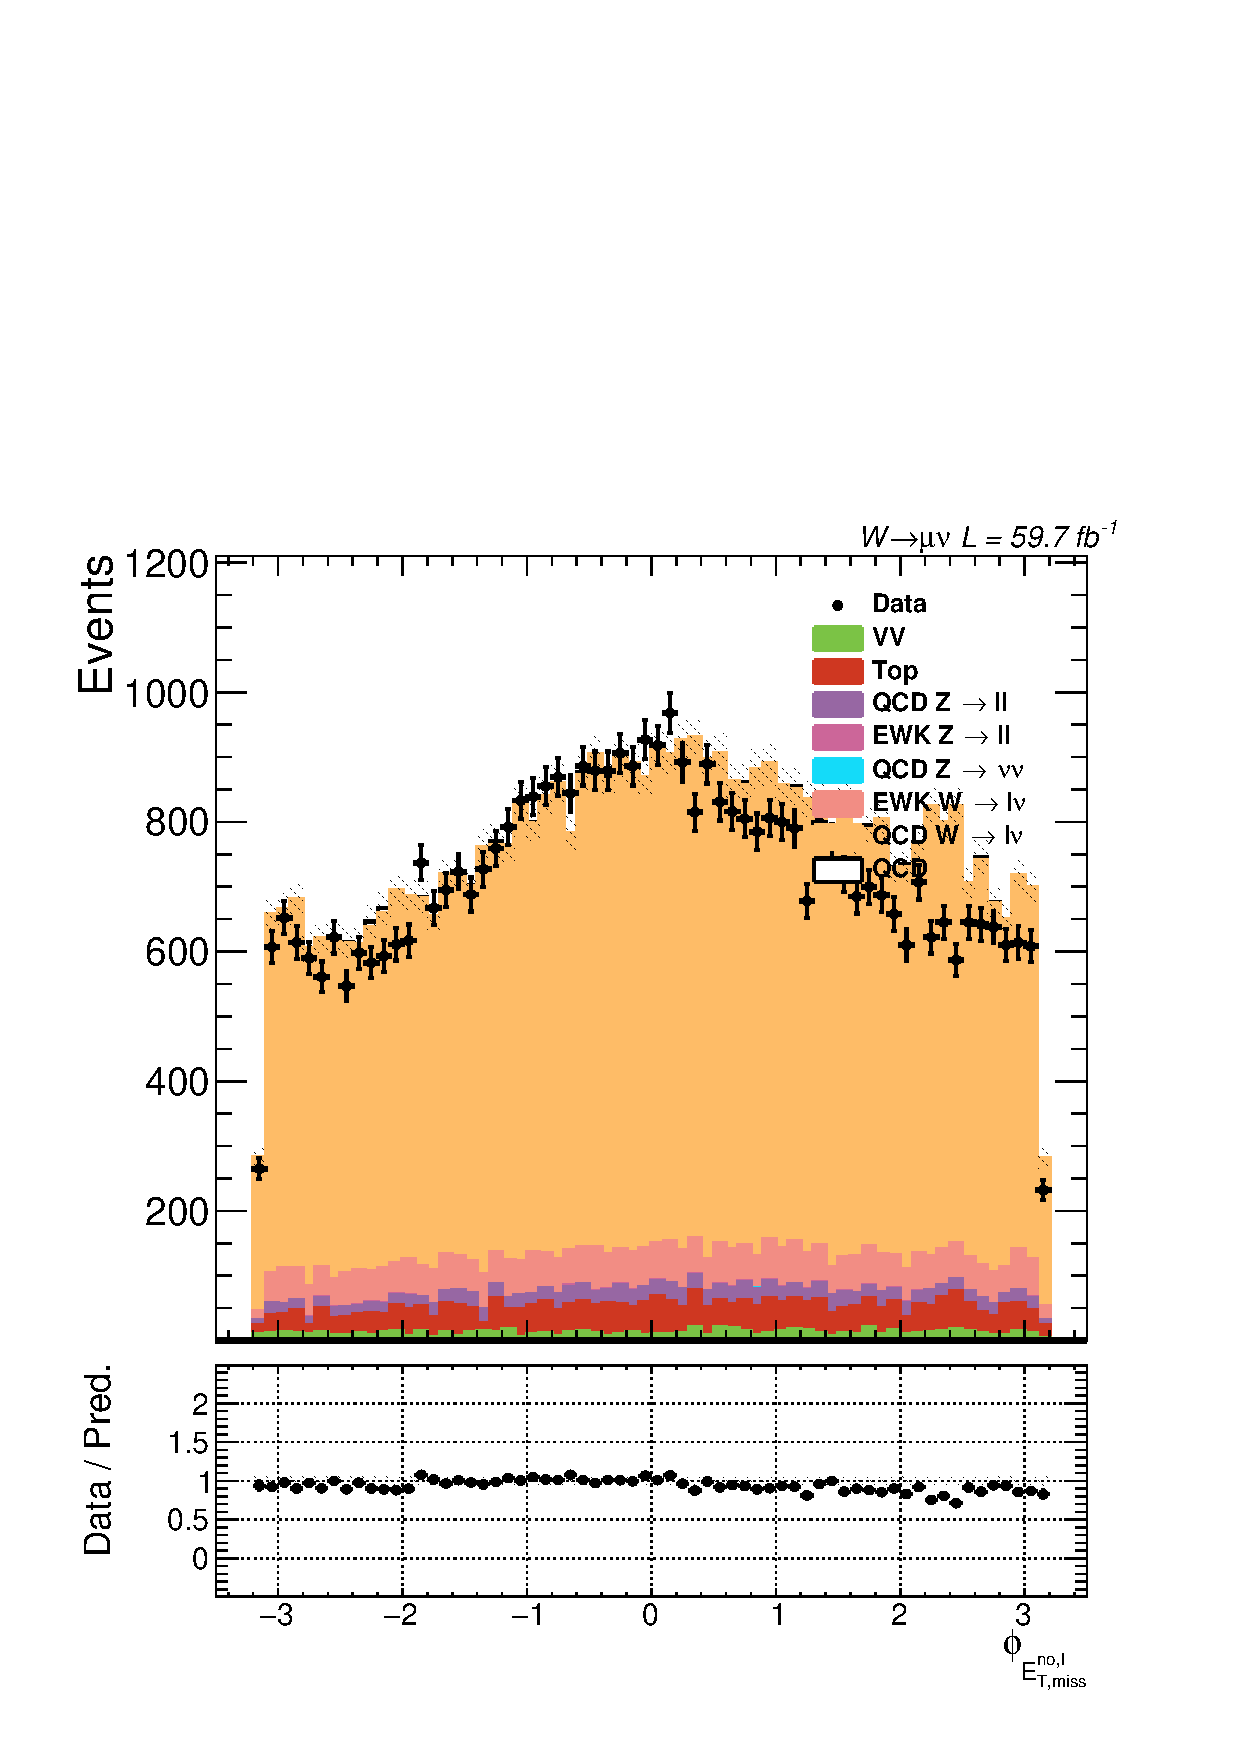
\includegraphics[width=0.47\textwidth]{Control_Regions/2018_MTR/Wmunu/MetNoMu_phi.pdf}
    }\\
    \subfigure[$\phi_{j1}$ - MTR]{
    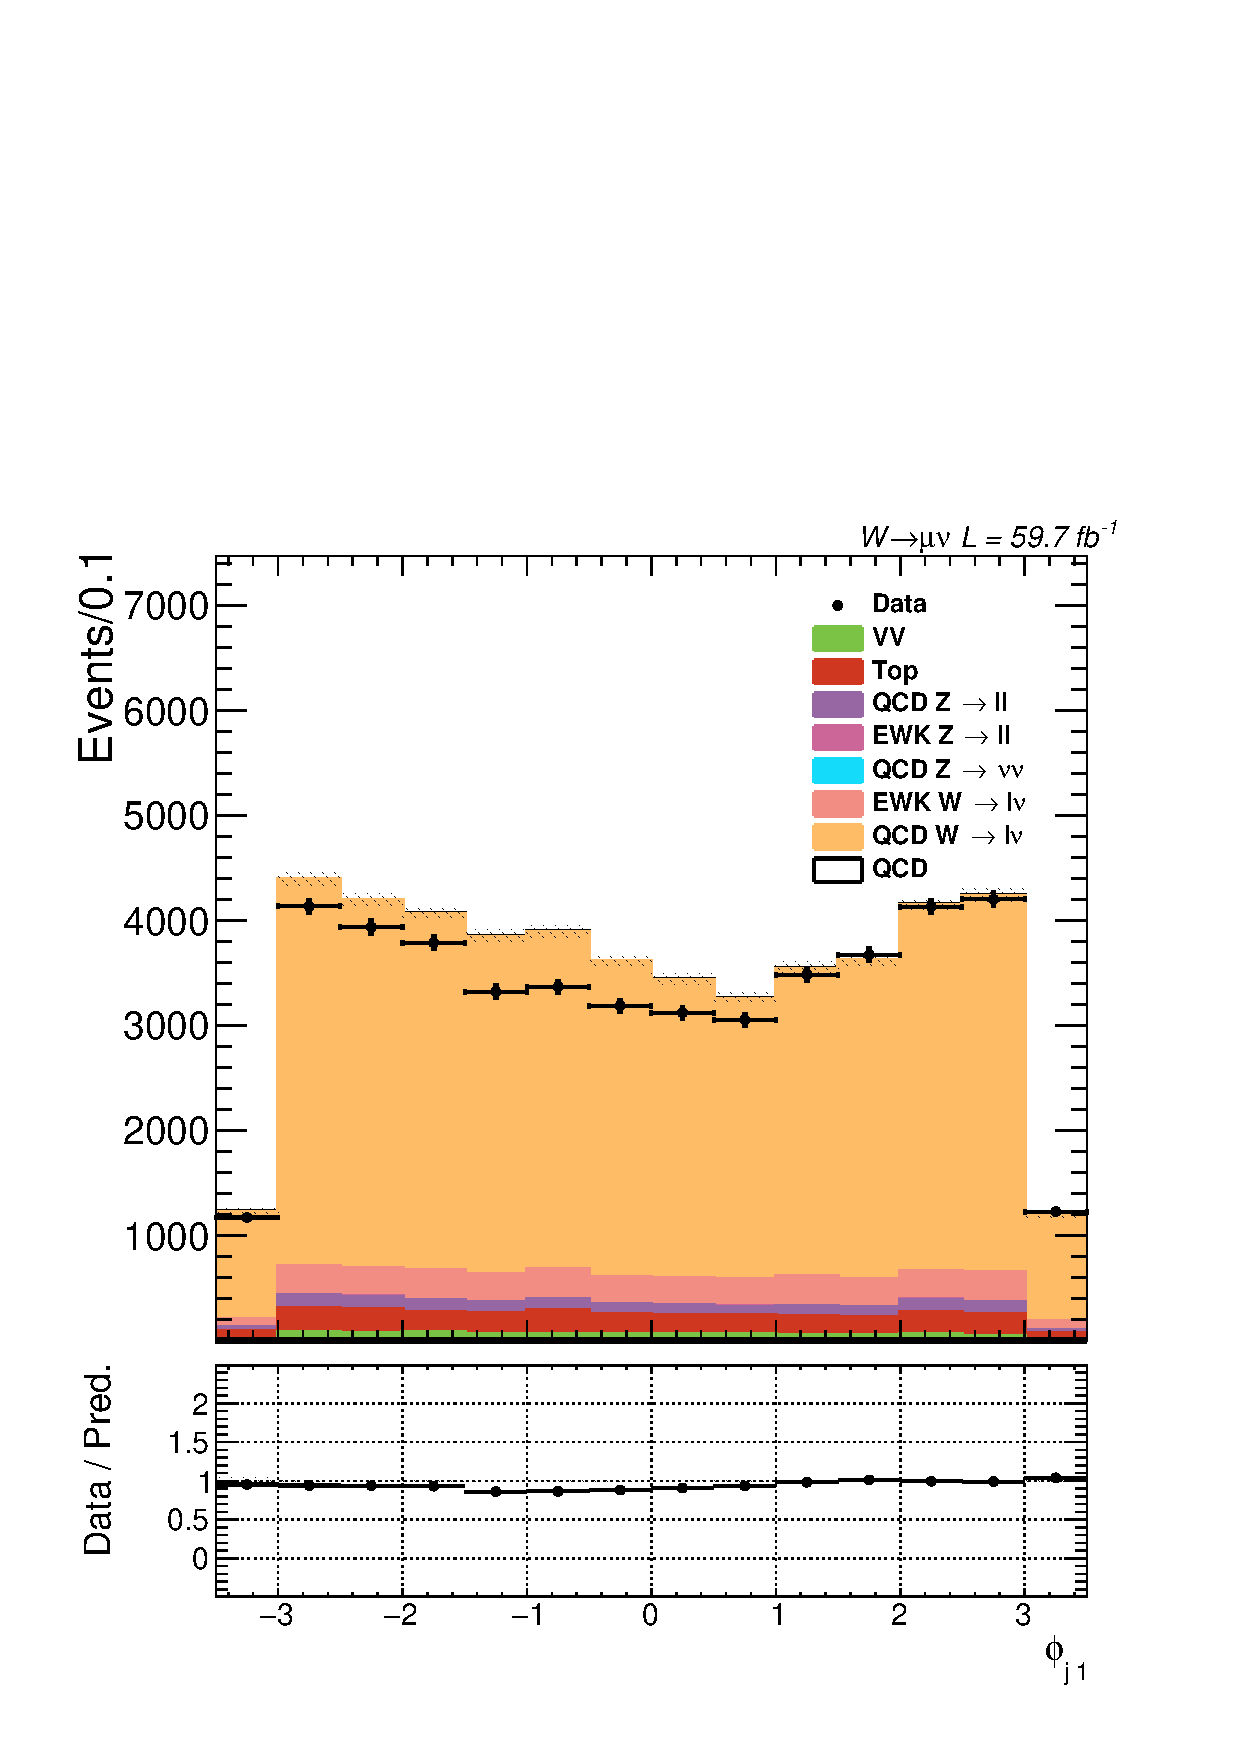
\includegraphics[width=0.47\textwidth]{Control_Regions/2018_MTR/Wmunu/Leading_jet_phi.pdf}
    }
  \caption{Distributions of $E_{T,miss}$ (a) and $\phi_{j1}$ (b) variables in the single muon CR for the MTR 2018 category, showing the absence of effects related to the HEM problem. }
  \label{app:Wmunu_noHEM}
\end{figure}




\begin{figure}[htbp]
  \centering
    \subfigure[$p_{T_{\mu,1}}$ - MTR]{
    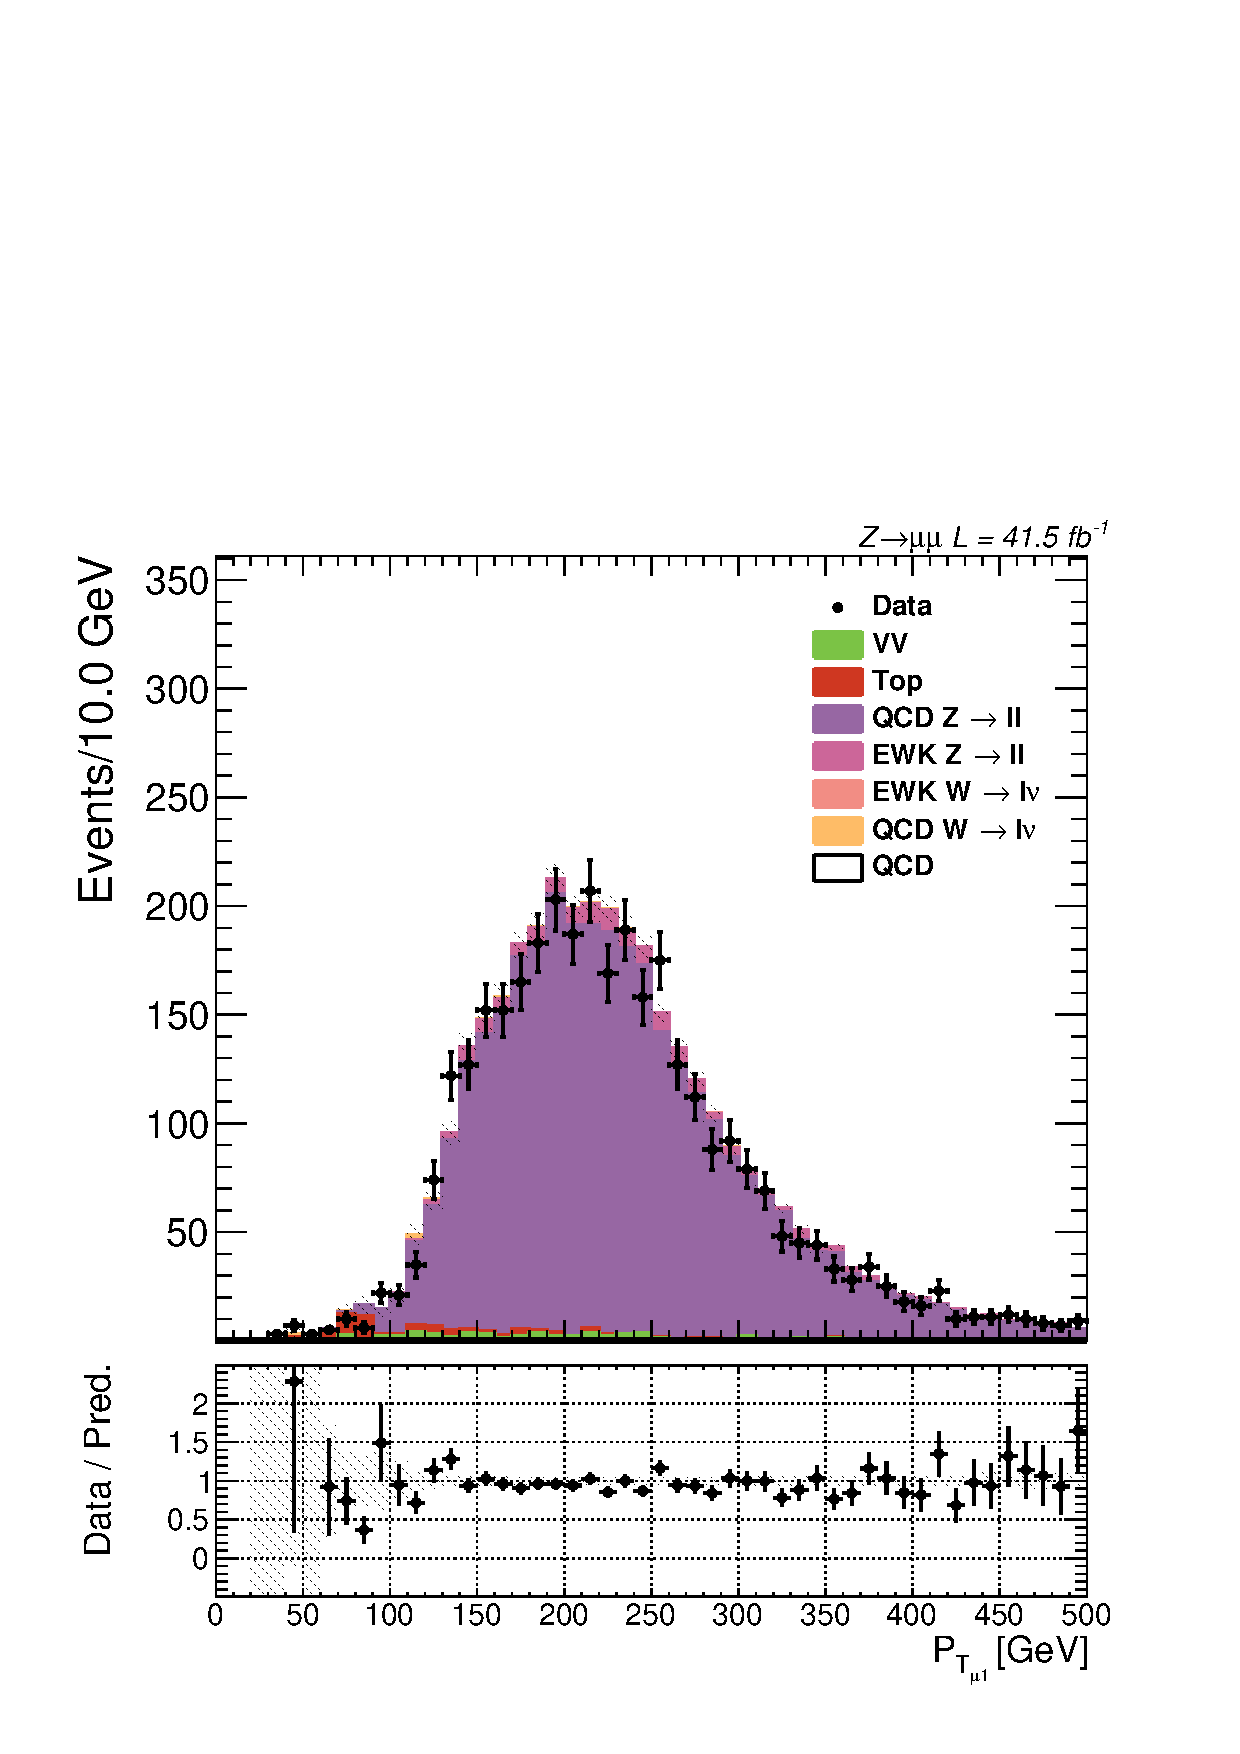
\includegraphics[width=0.49\textwidth]{Control_Regions/2017_MTR/Zmumu/Leading_muon_pt.pdf}
    }
    \subfigure[$\eta_{\mu,1}$ - MTR]{
    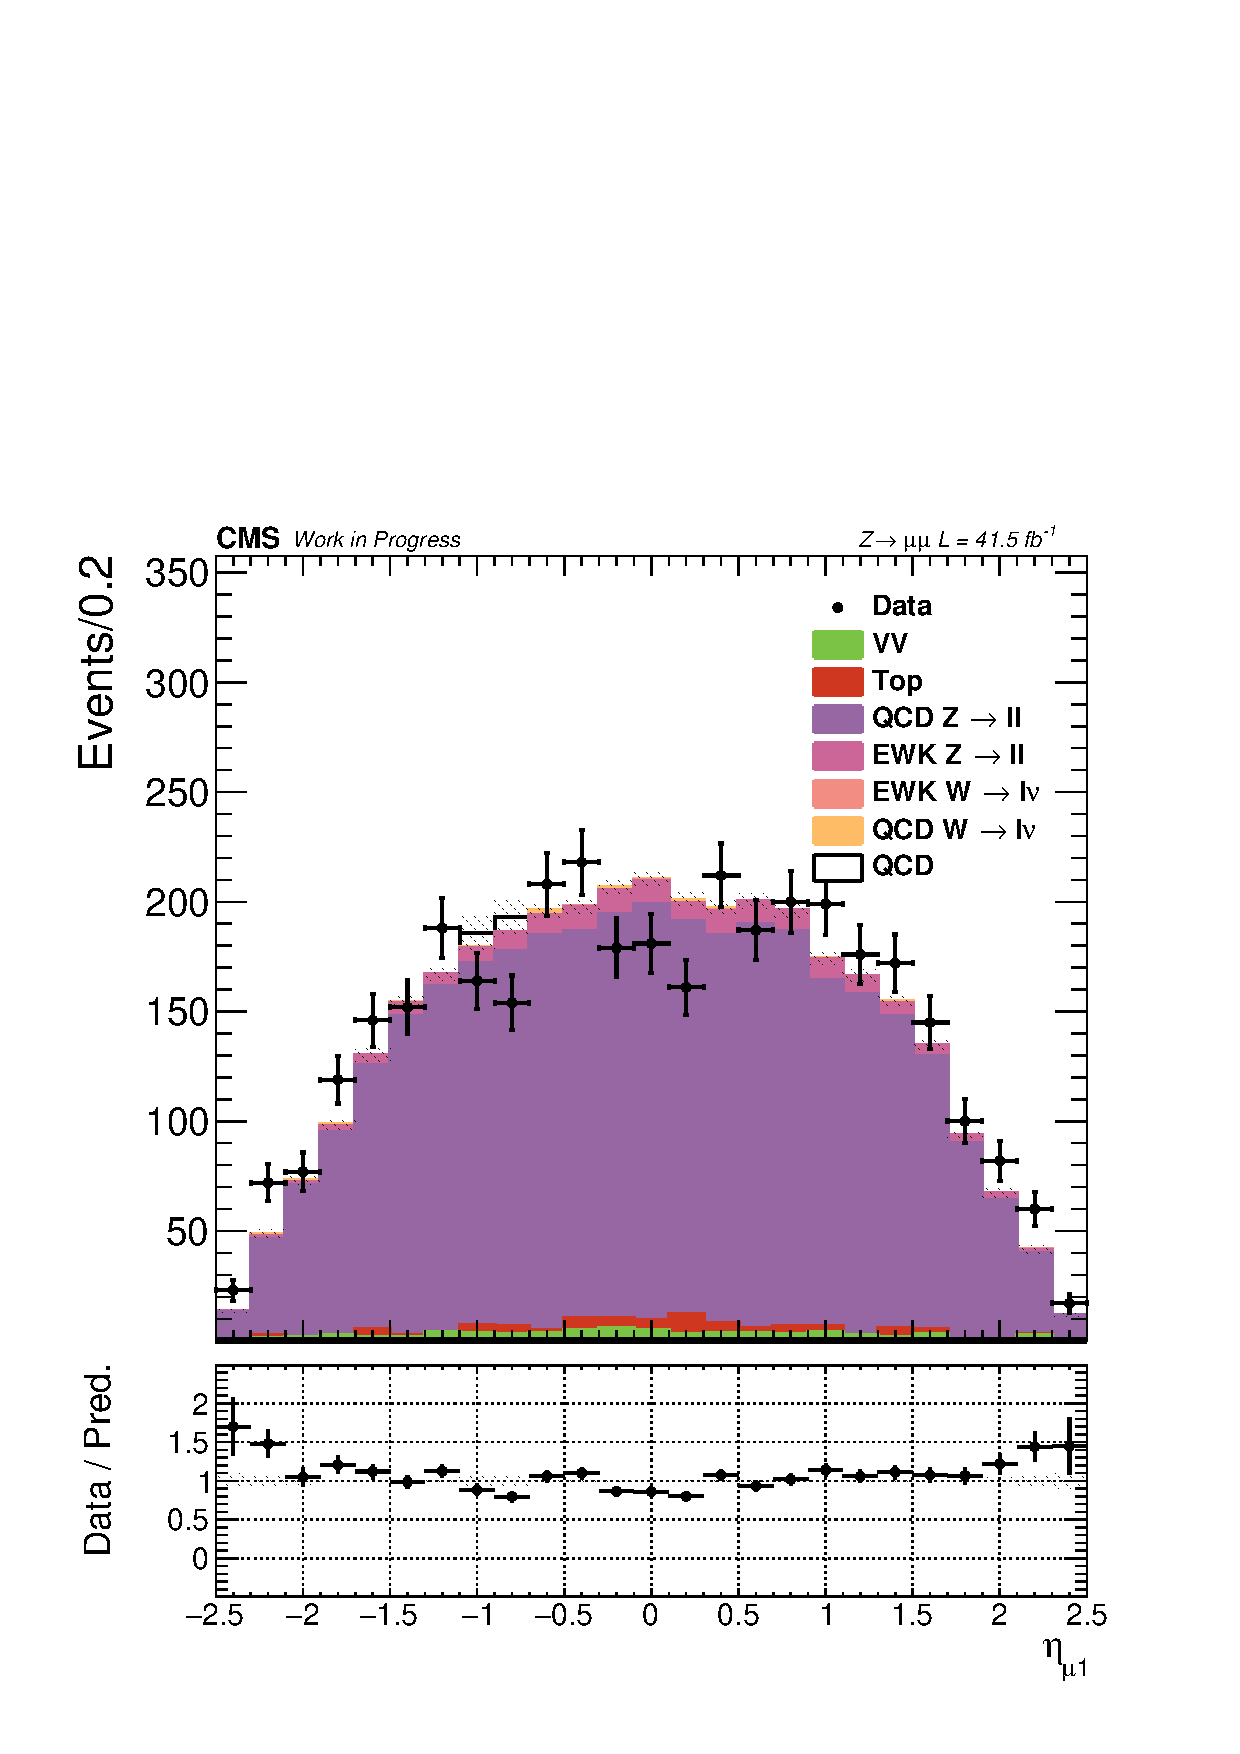
\includegraphics[width=0.49\textwidth]{Control_Regions/2017_MTR/Zmumu/Leading_muon_eta.pdf}
    }\\
    \subfigure[$p_{T_{\mu,1}}$ - VTR]{
    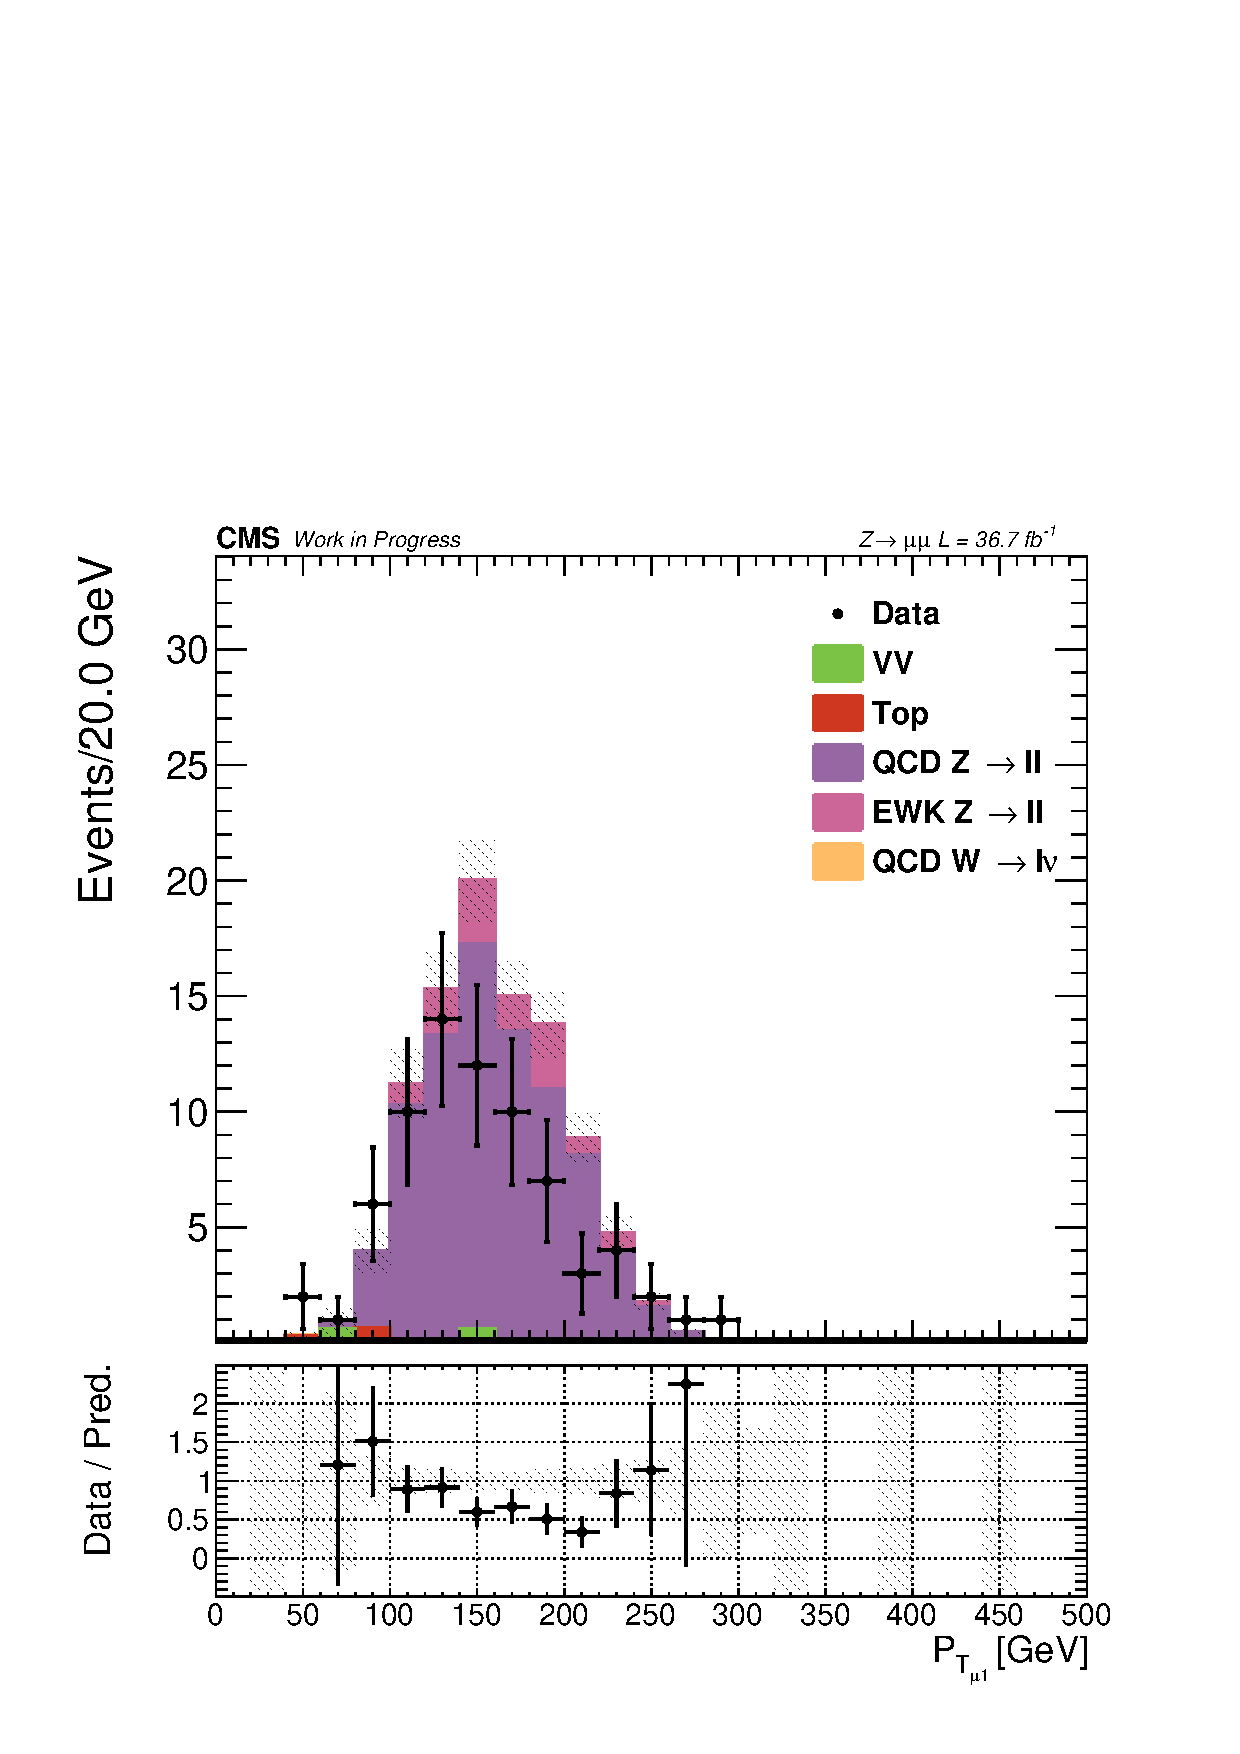
\includegraphics[width=0.49\textwidth]{Control_Regions/2017_VTR/Zmumu/Leading_muon_pt.pdf}
    }
    \subfigure[$\eta_{\mu,1}$  - VTR]{
    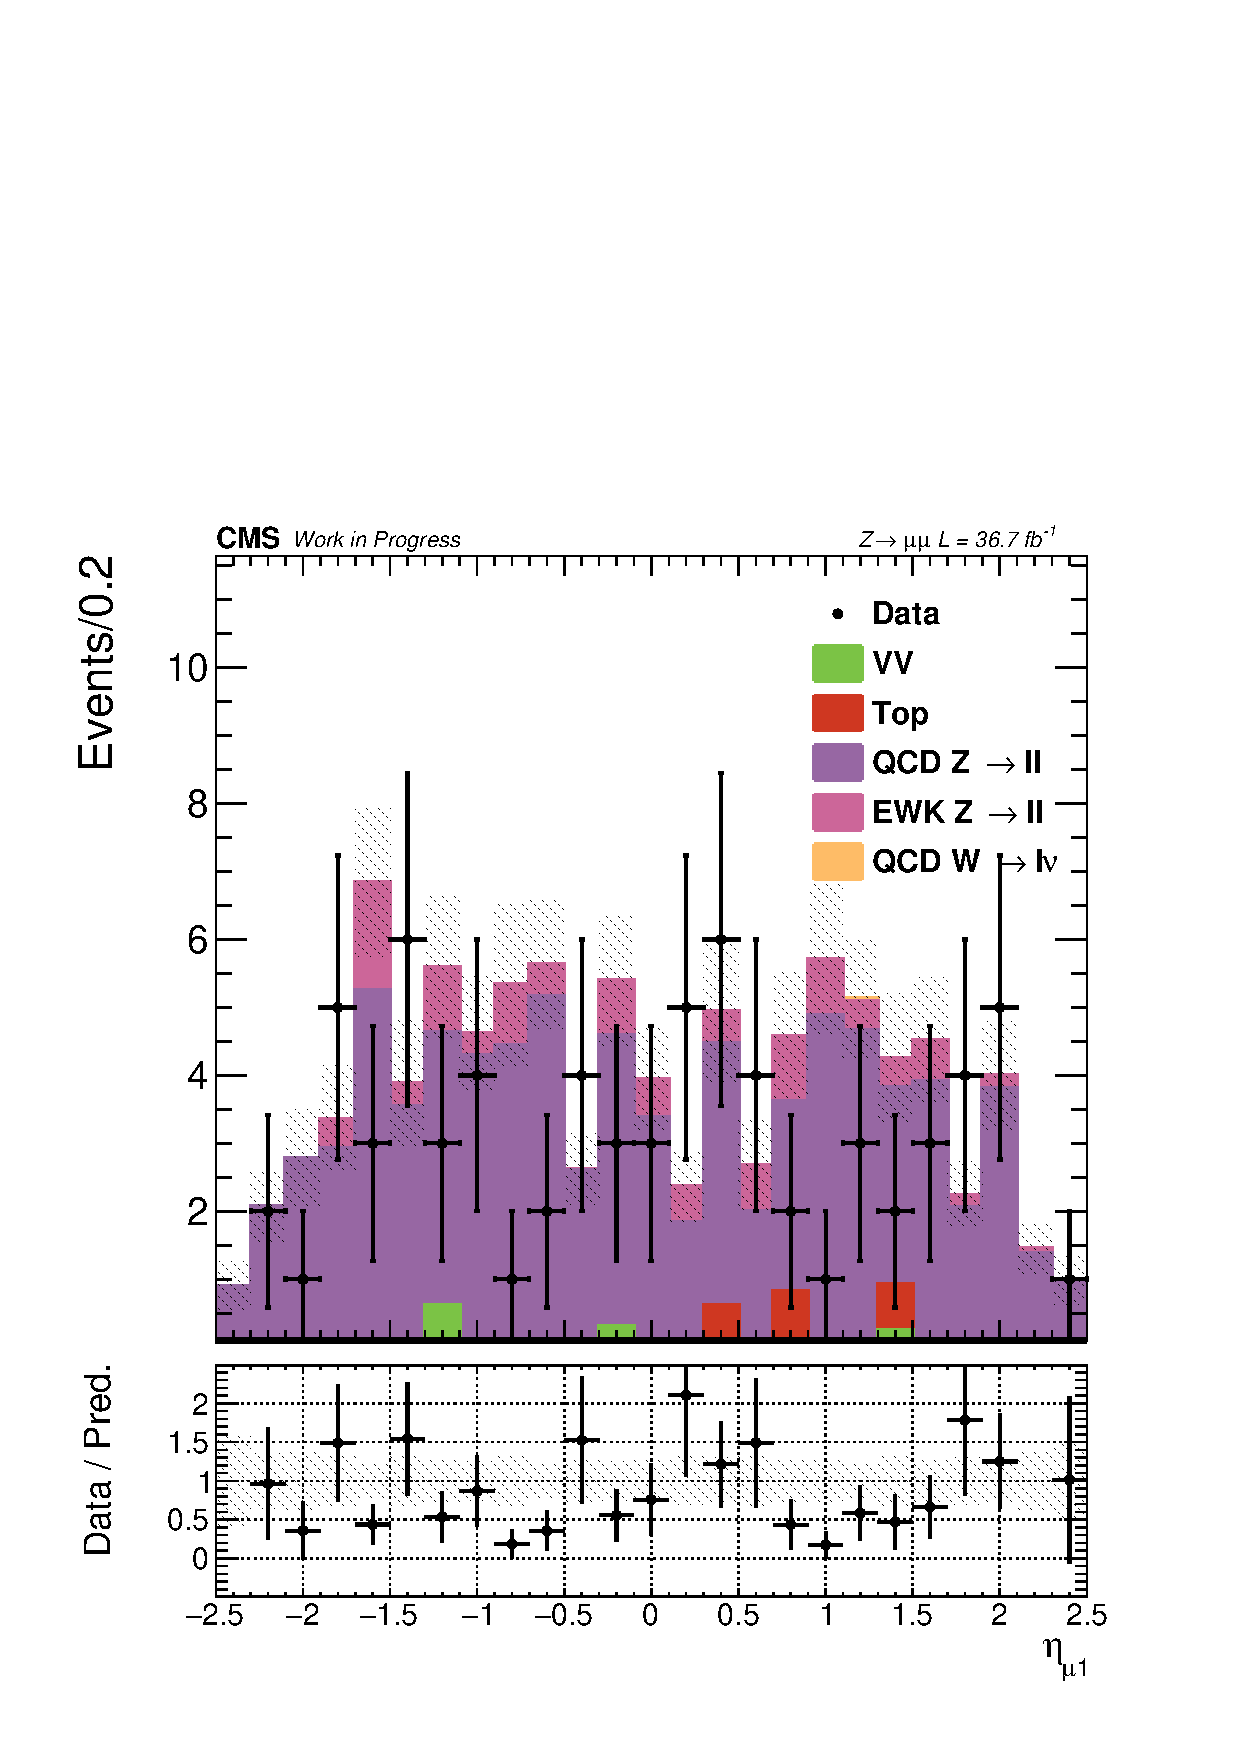
\includegraphics[width=0.49\textwidth]{Control_Regions/2017_VTR/Zmumu/Leading_muon_eta.pdf}
    }
  \caption{Distributions of $p_{T_{\mu,1}}$ and $\eta_{\mu,1}$ variables in the double muon region for MTR (top) and VTR (bottom) categories for the 2017 era of data taking.}
  \label{app:2017_Zmumu_1}
\end{figure}

\begin{figure}[htbp]
  \centering
    \subfigure[$p_{T_{\mu,1}}$ - MTR]{
    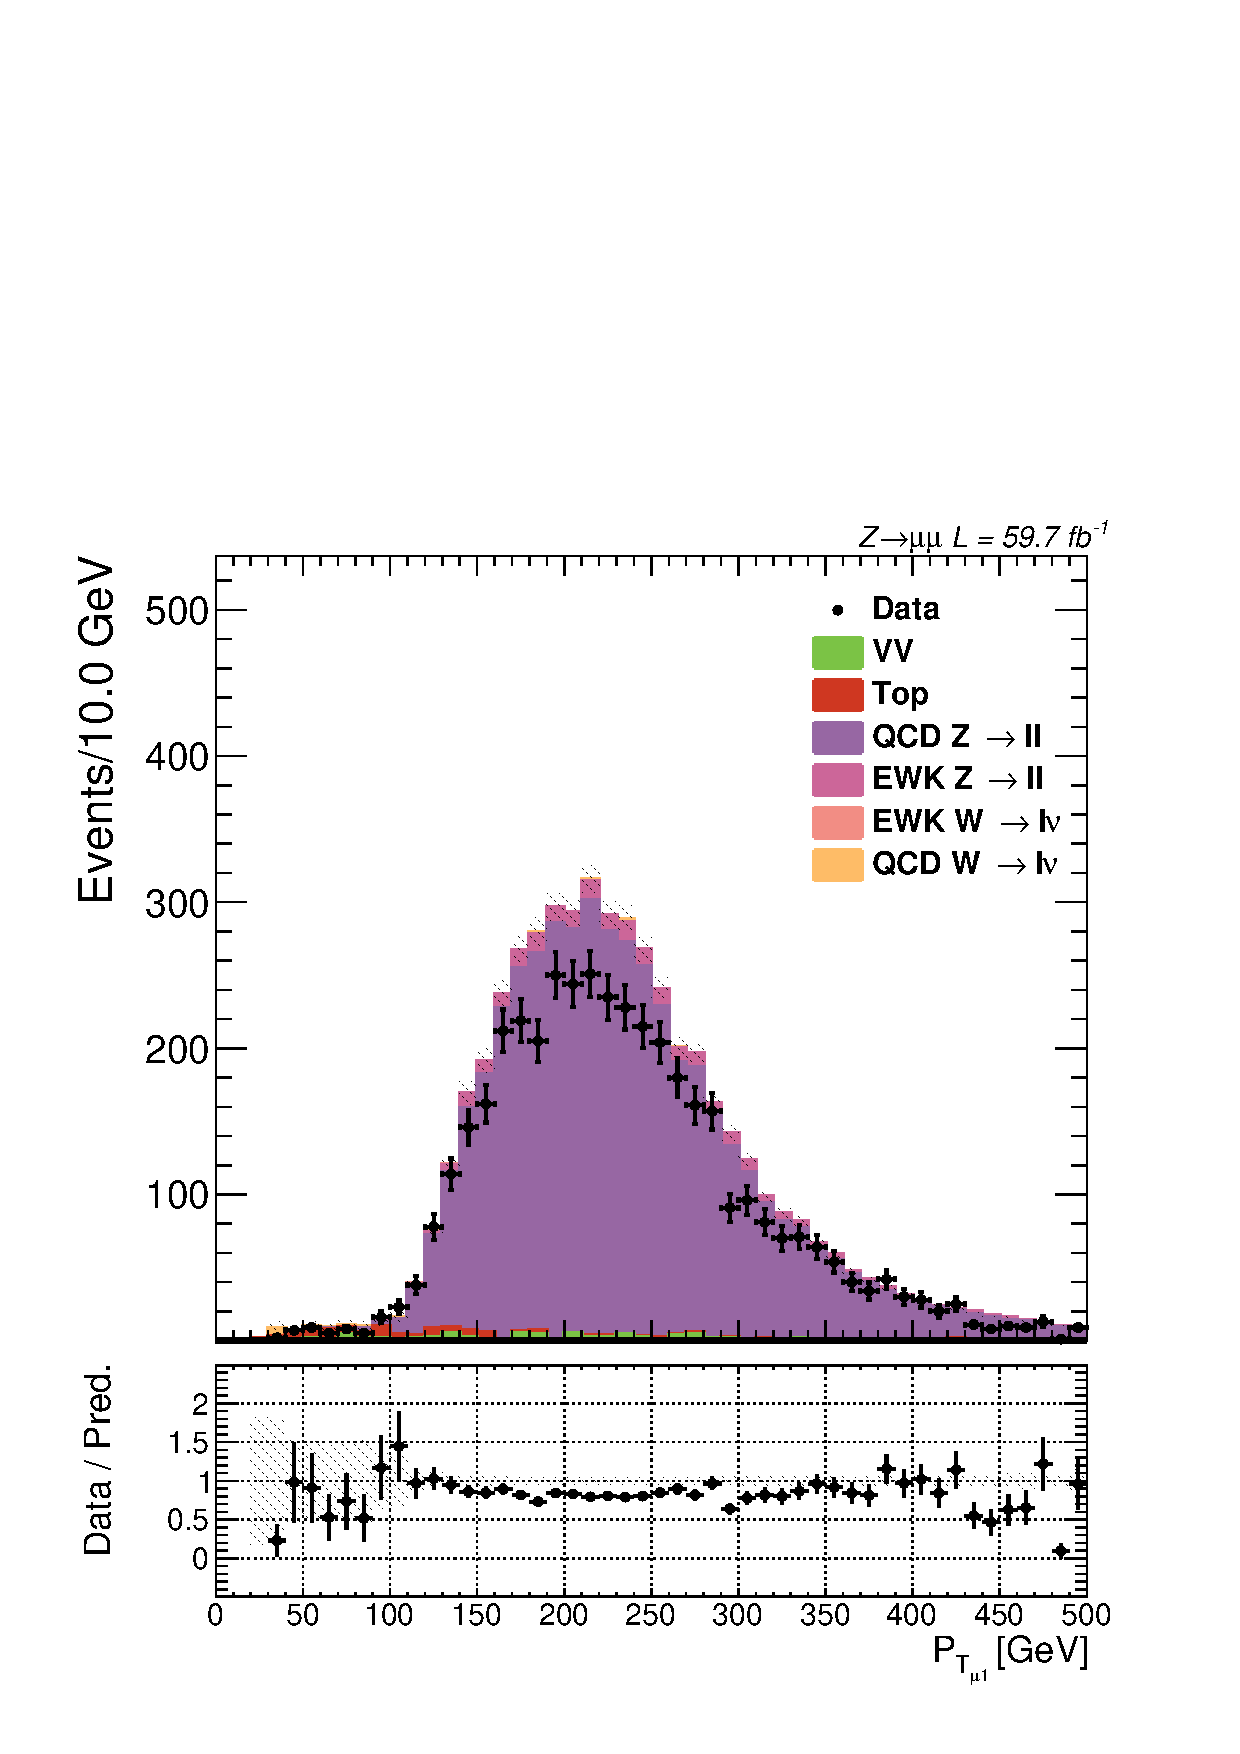
\includegraphics[width=0.49\textwidth]{Control_Regions/2018_MTR/Zmumu/Leading_muon_pt.pdf}
    }
    \subfigure[$\eta_{\mu,1}$ - MTR]{
    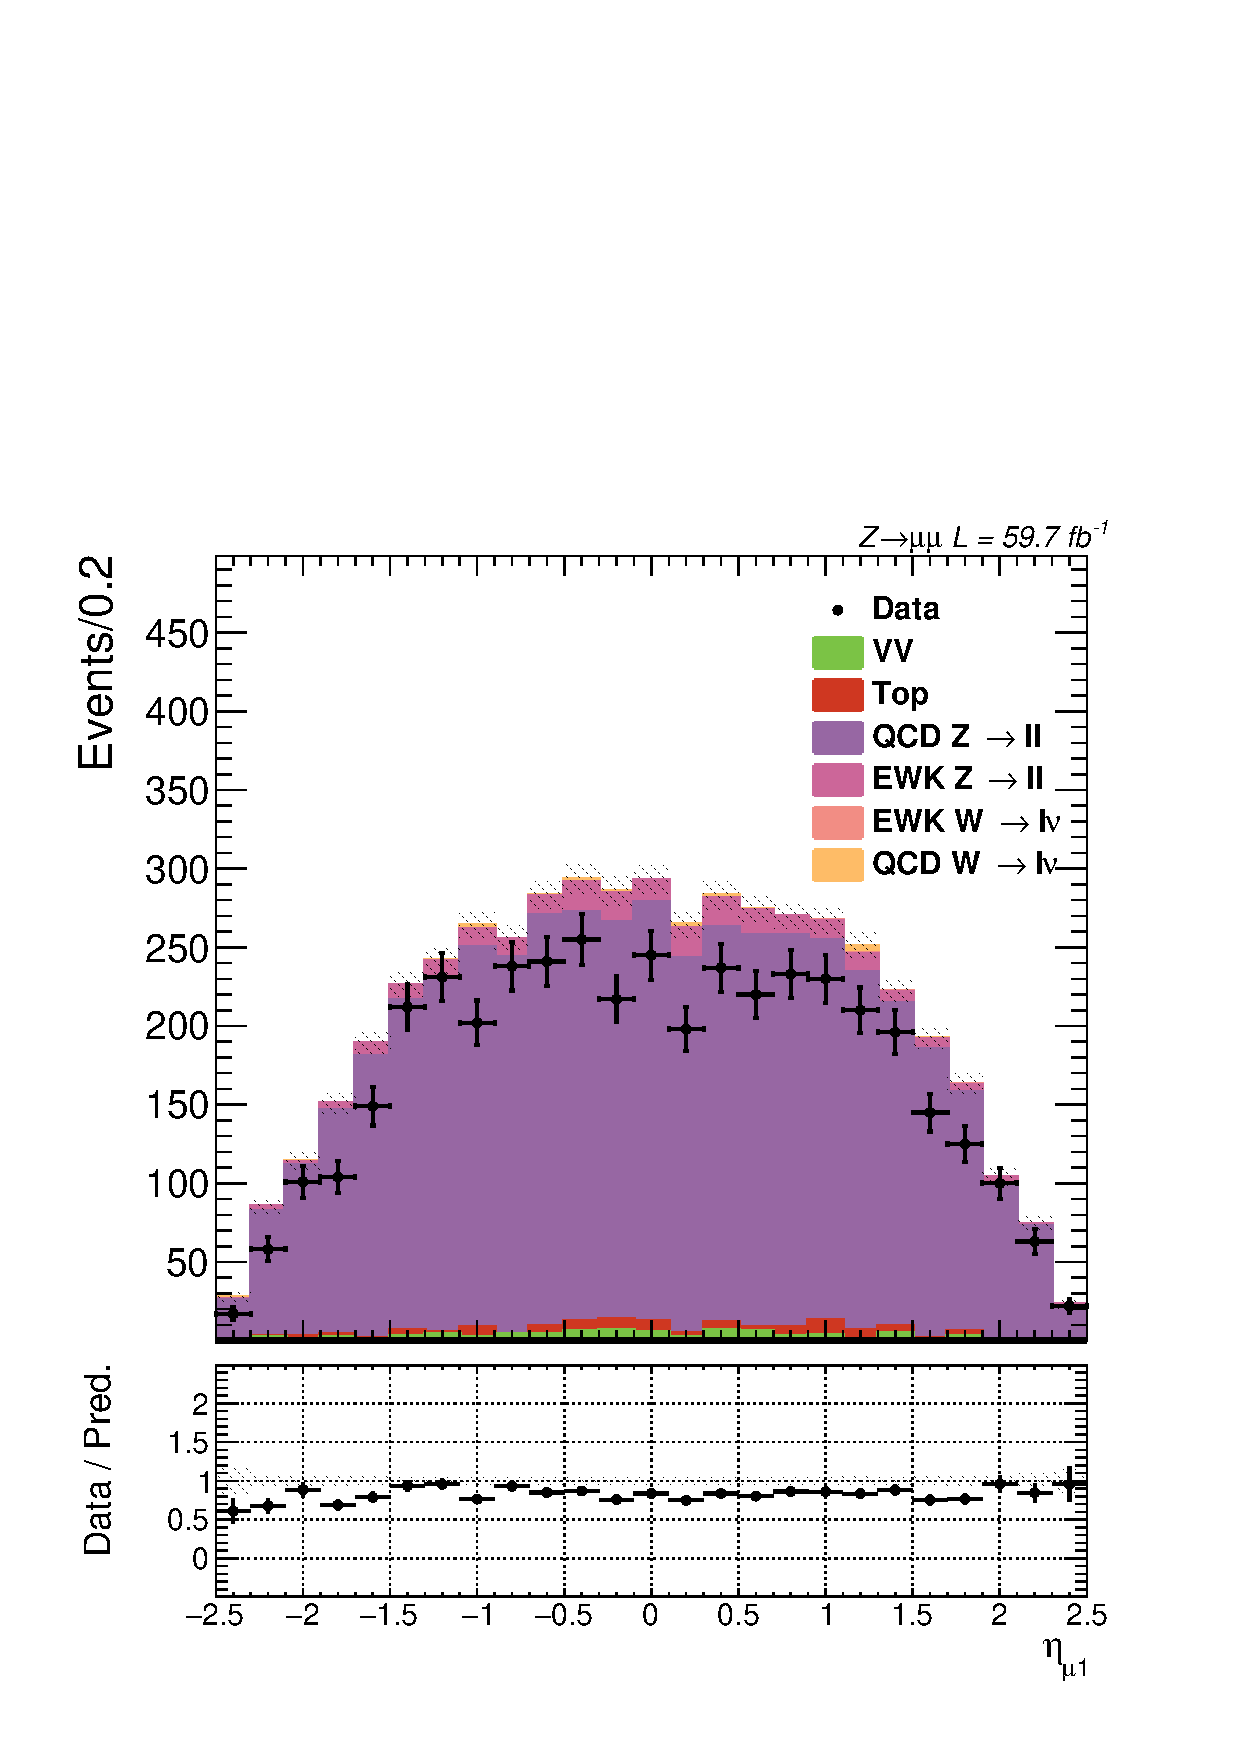
\includegraphics[width=0.49\textwidth]{Control_Regions/2018_MTR/Zmumu/Leading_muon_eta.pdf}
    }\\
    \subfigure[$p_{T_{\mu,1}}$ - VTR]{
    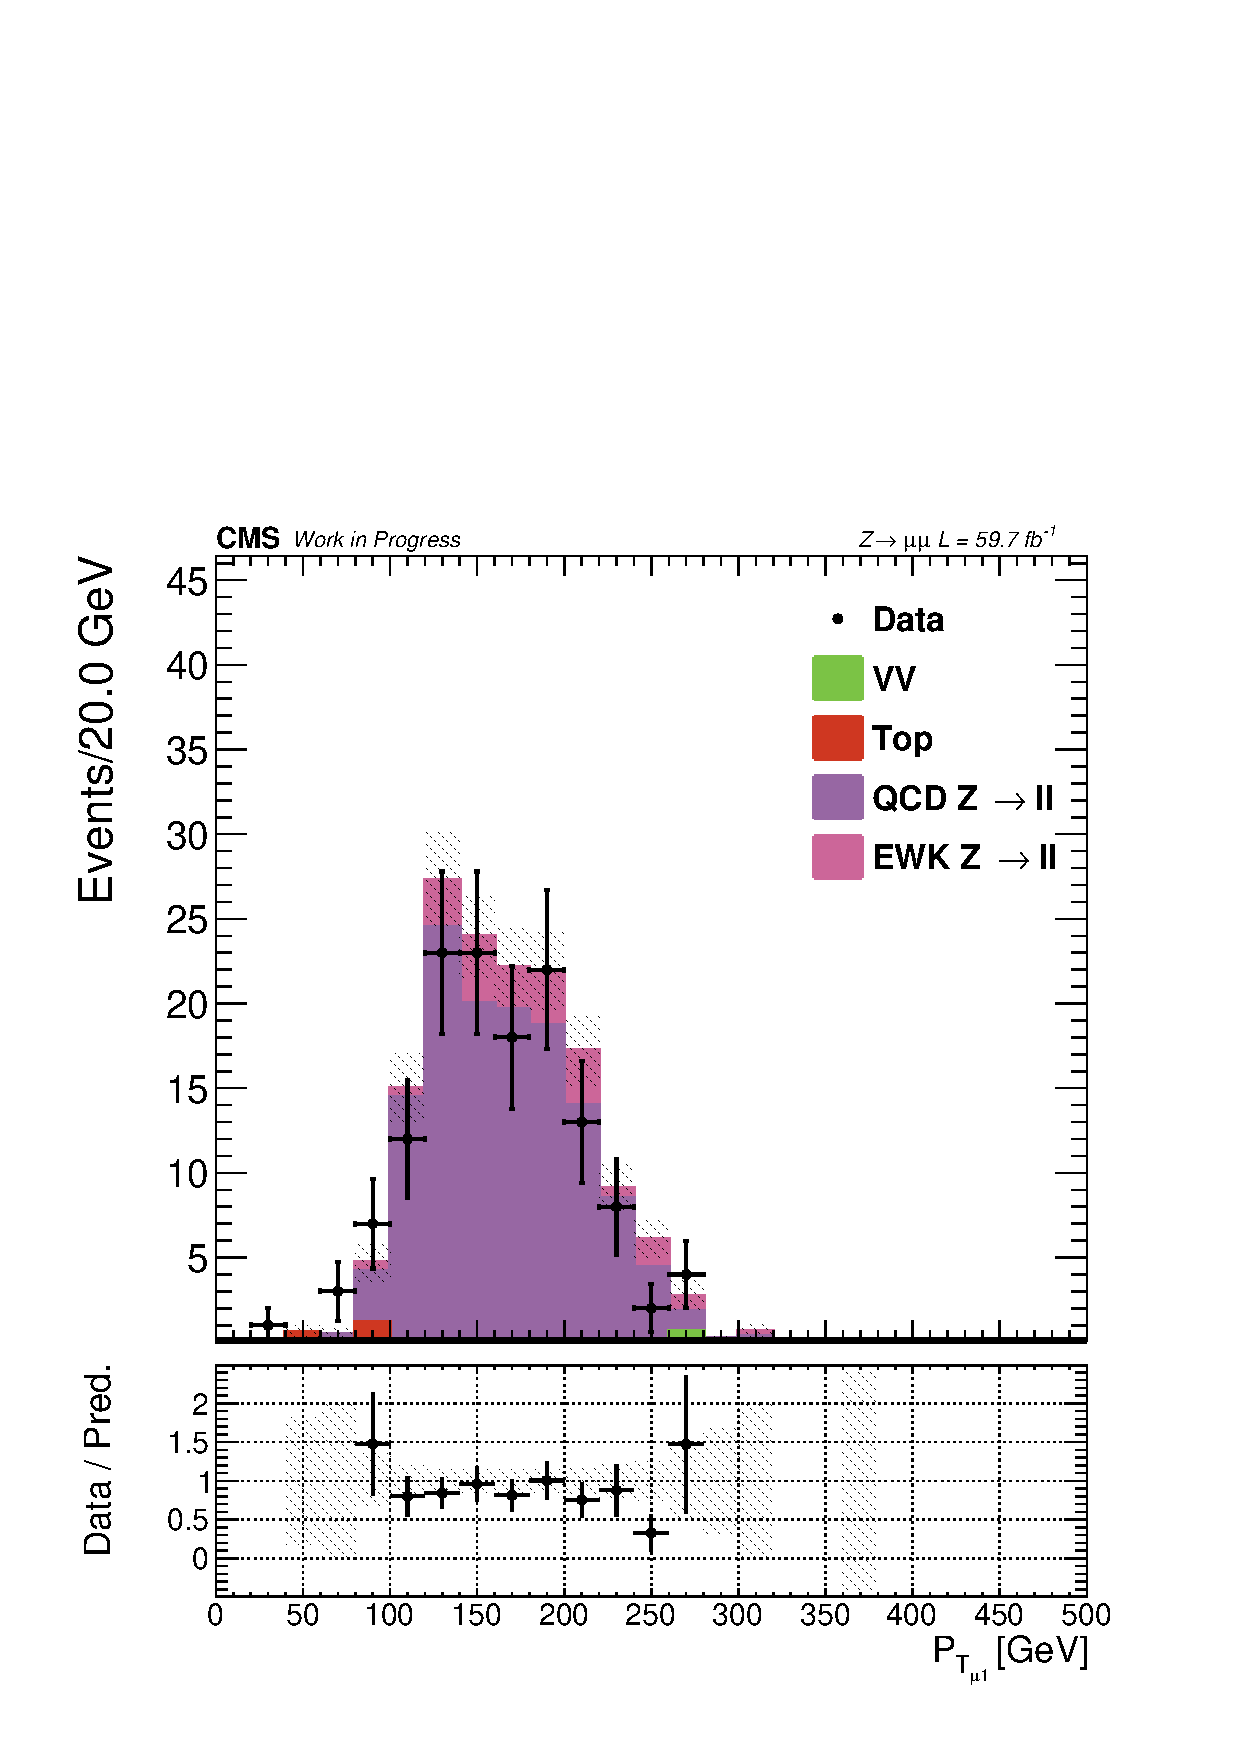
\includegraphics[width=0.49\textwidth]{Control_Regions/2018_VTR/Zmumu/Leading_muon_pt.pdf}
    }
    \subfigure[$\eta_{\mu,1}$  - VTR]{
    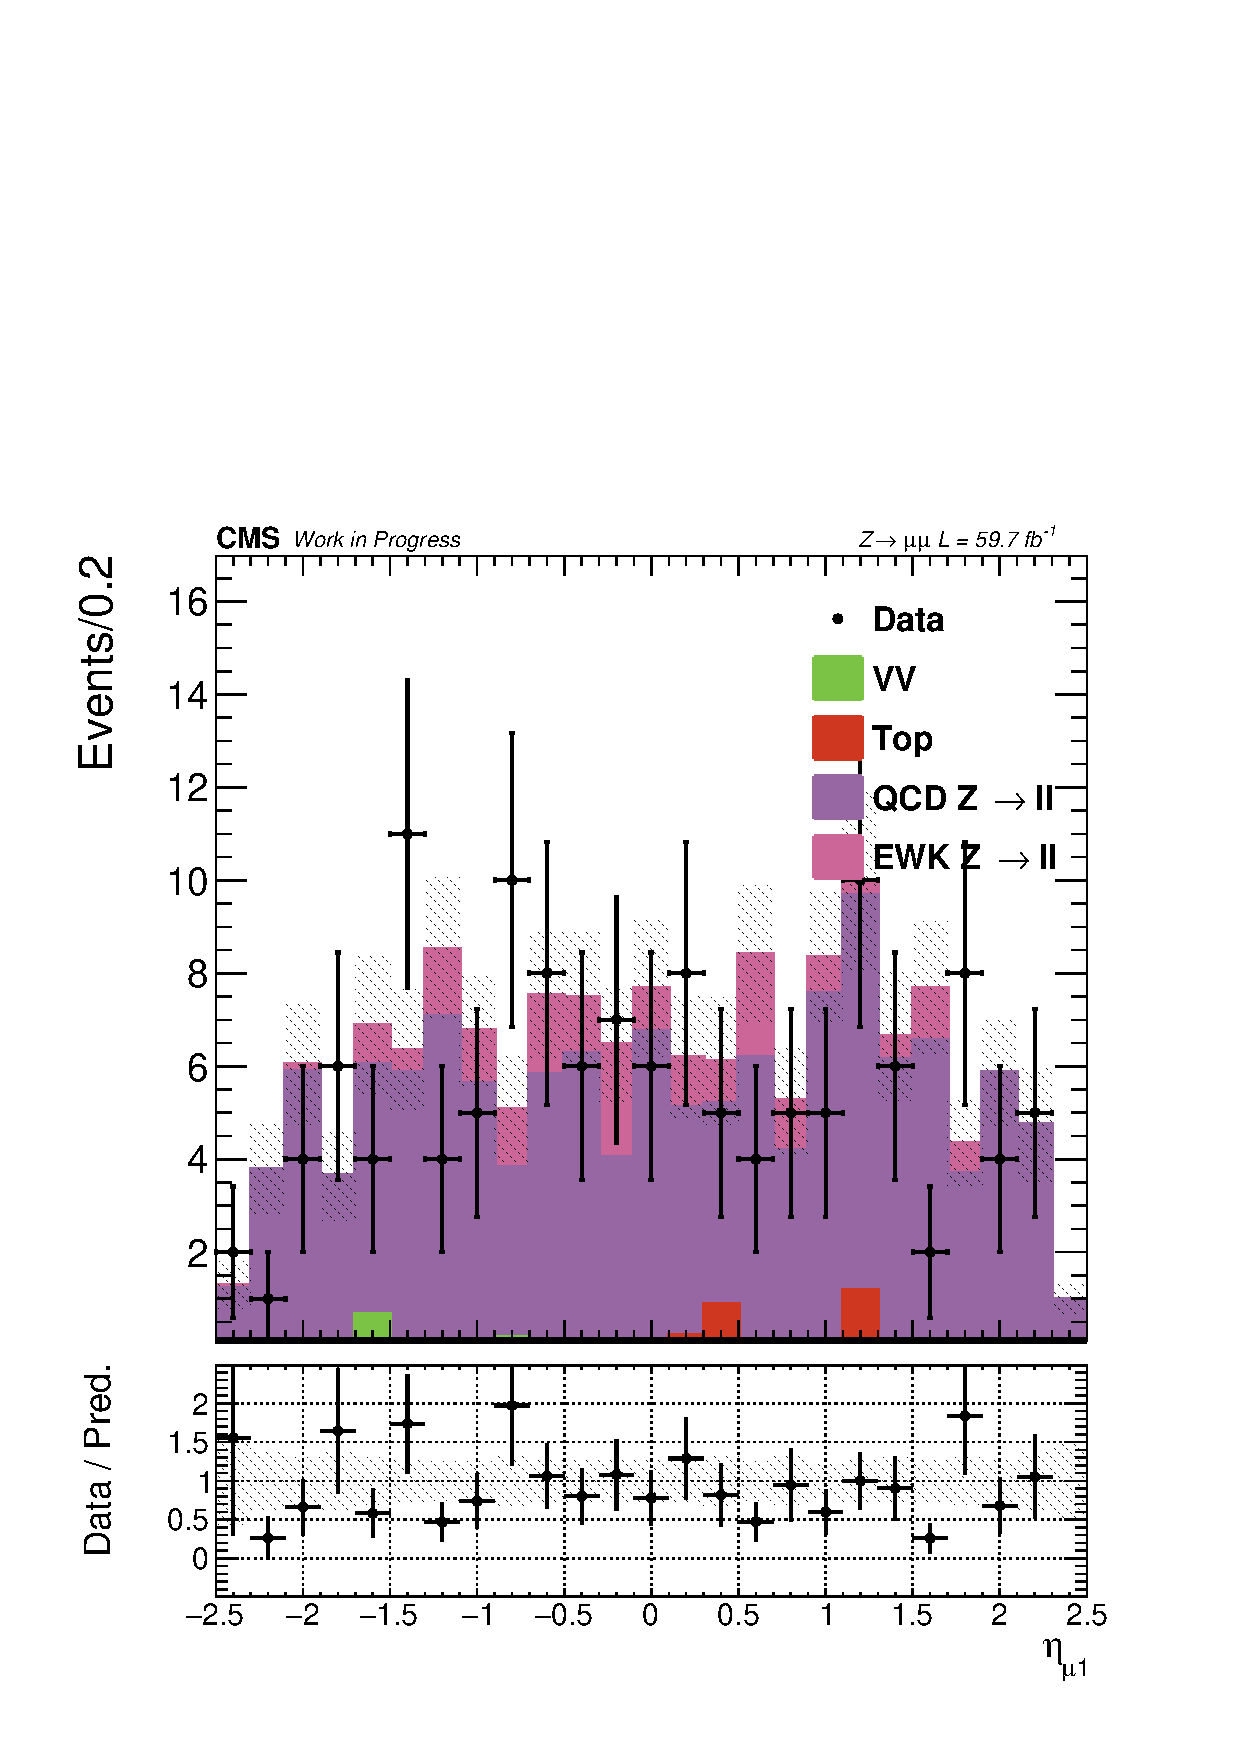
\includegraphics[width=0.49\textwidth]{Control_Regions/2018_VTR/Zmumu/Leading_muon_eta.pdf}
    }
  \caption{Distributions of $p_{T_{\mu,1}}$and $\eta_{\mu,1}$ variables in the double muon region for MTR (top) and VTR (bottom) categories for the 2018 era of data taking.}
  \label{app:2018_Zmumu_1}
\end{figure}

\begin{figure}[htbp]
  \centering
    \subfigure[$p_{T_{\mu,1}}$ - VTR]{
    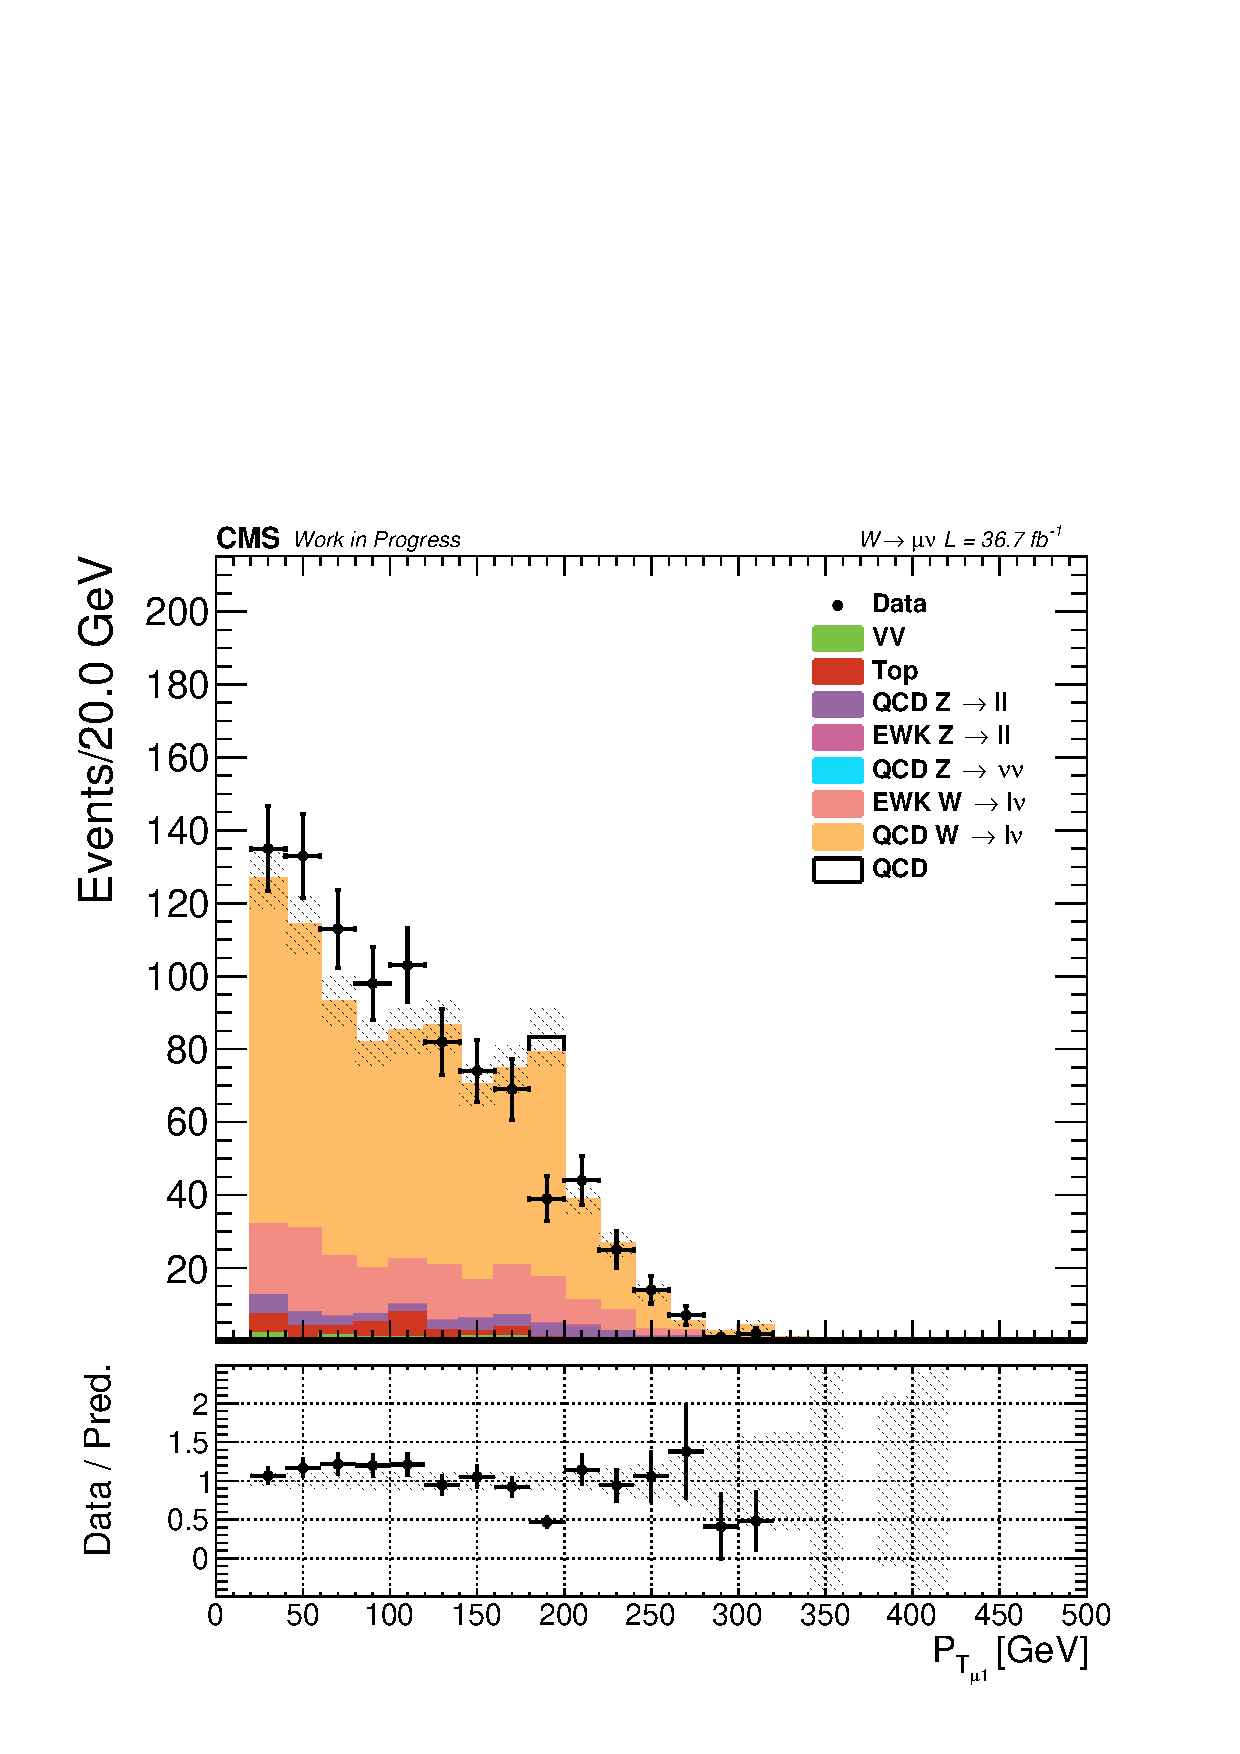
\includegraphics[width=0.49\textwidth]{Control_Regions/2017_VTR/Wmunu/Leading_muon_pt.pdf}
    }\\
    \subfigure[$\eta_{\mu,1}$  - VTR]{
    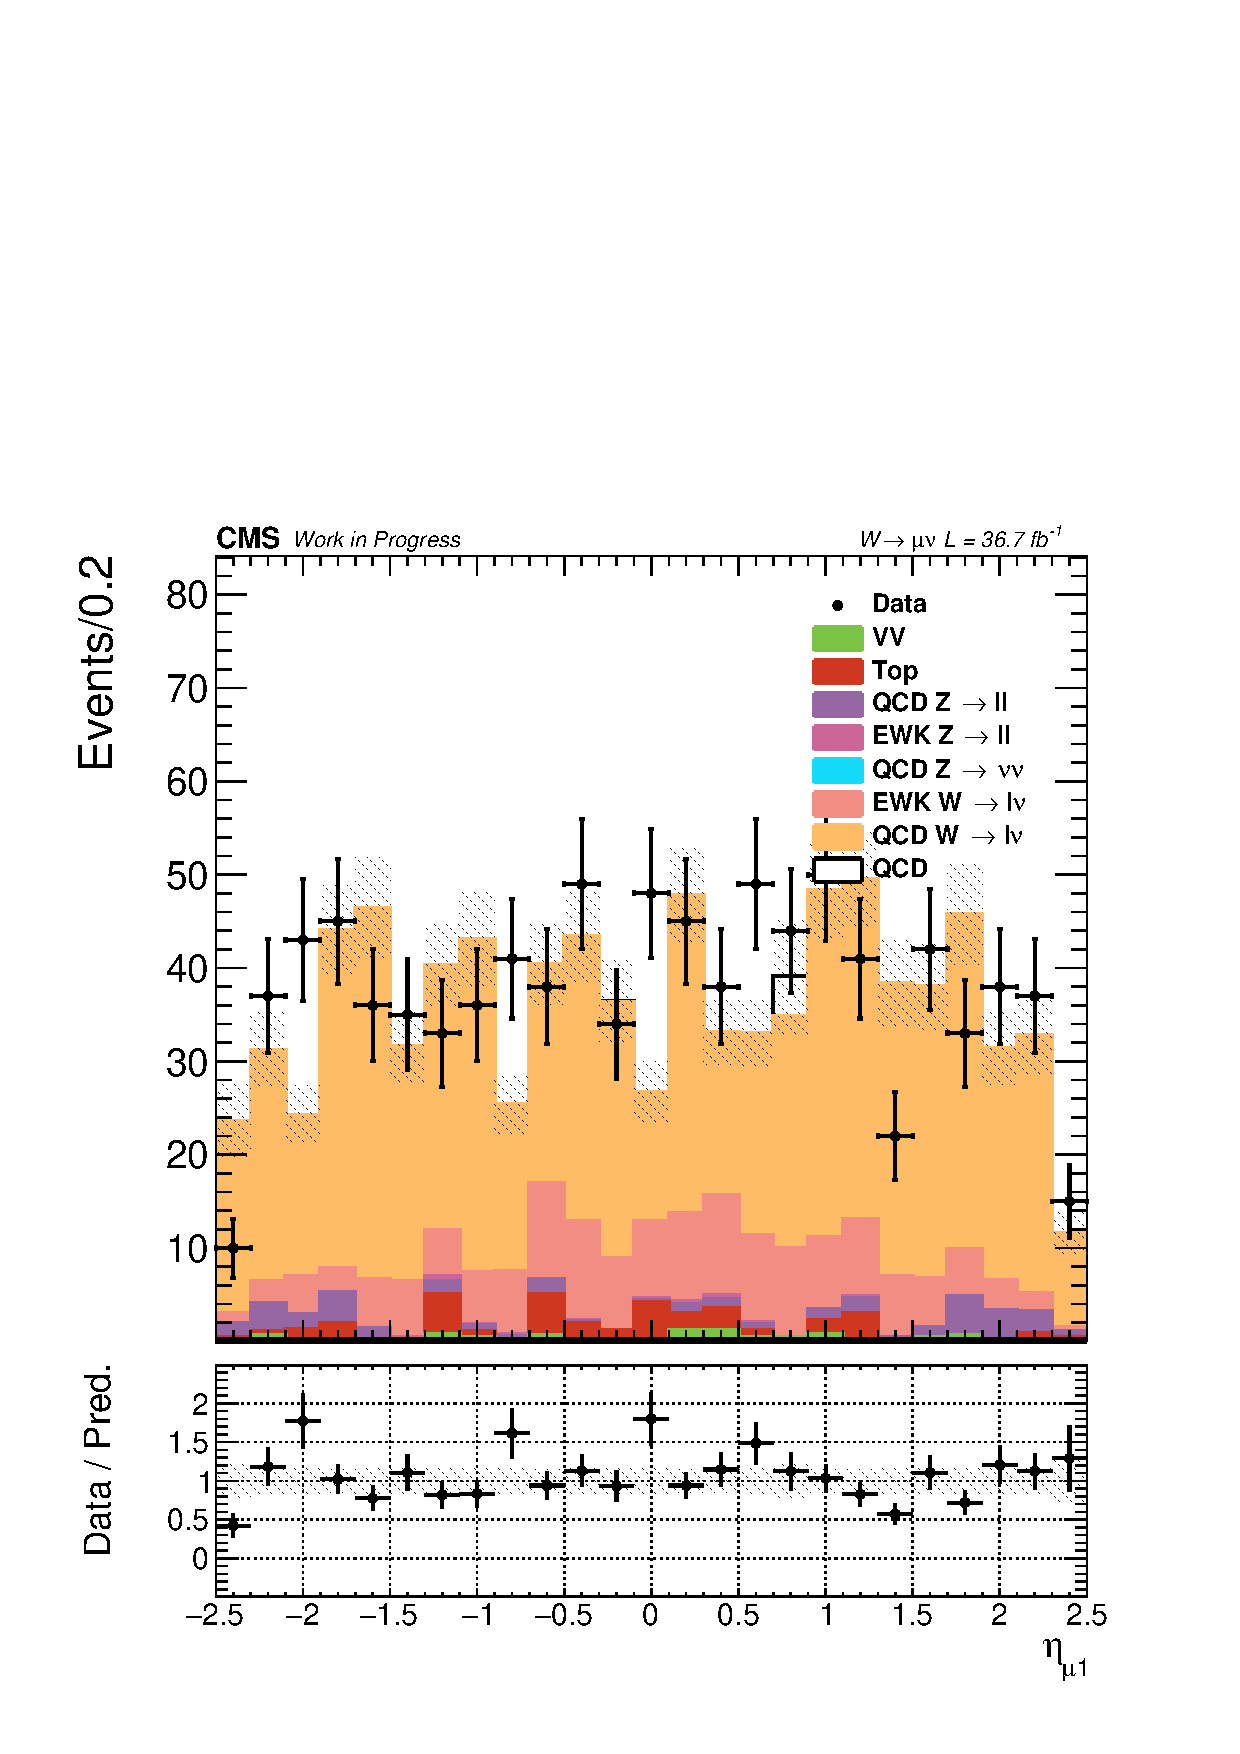
\includegraphics[width=0.49\textwidth]{Control_Regions/2017_VTR/Wmunu/Leading_muon_eta.pdf}
    }
  \caption{Distributions of $p_{T_{\mu,1}}$and $\eta_{\mu,1}$ variables in the single muon region for the VTR category for the 2017 era of data taking.}
  \label{app:2017_Wmunu_1}
\end{figure}
\newpage

\begin{figure}[htbp]
  \centering
    \subfigure[$p_{T_{\mu,1}}$ - MTR]{
    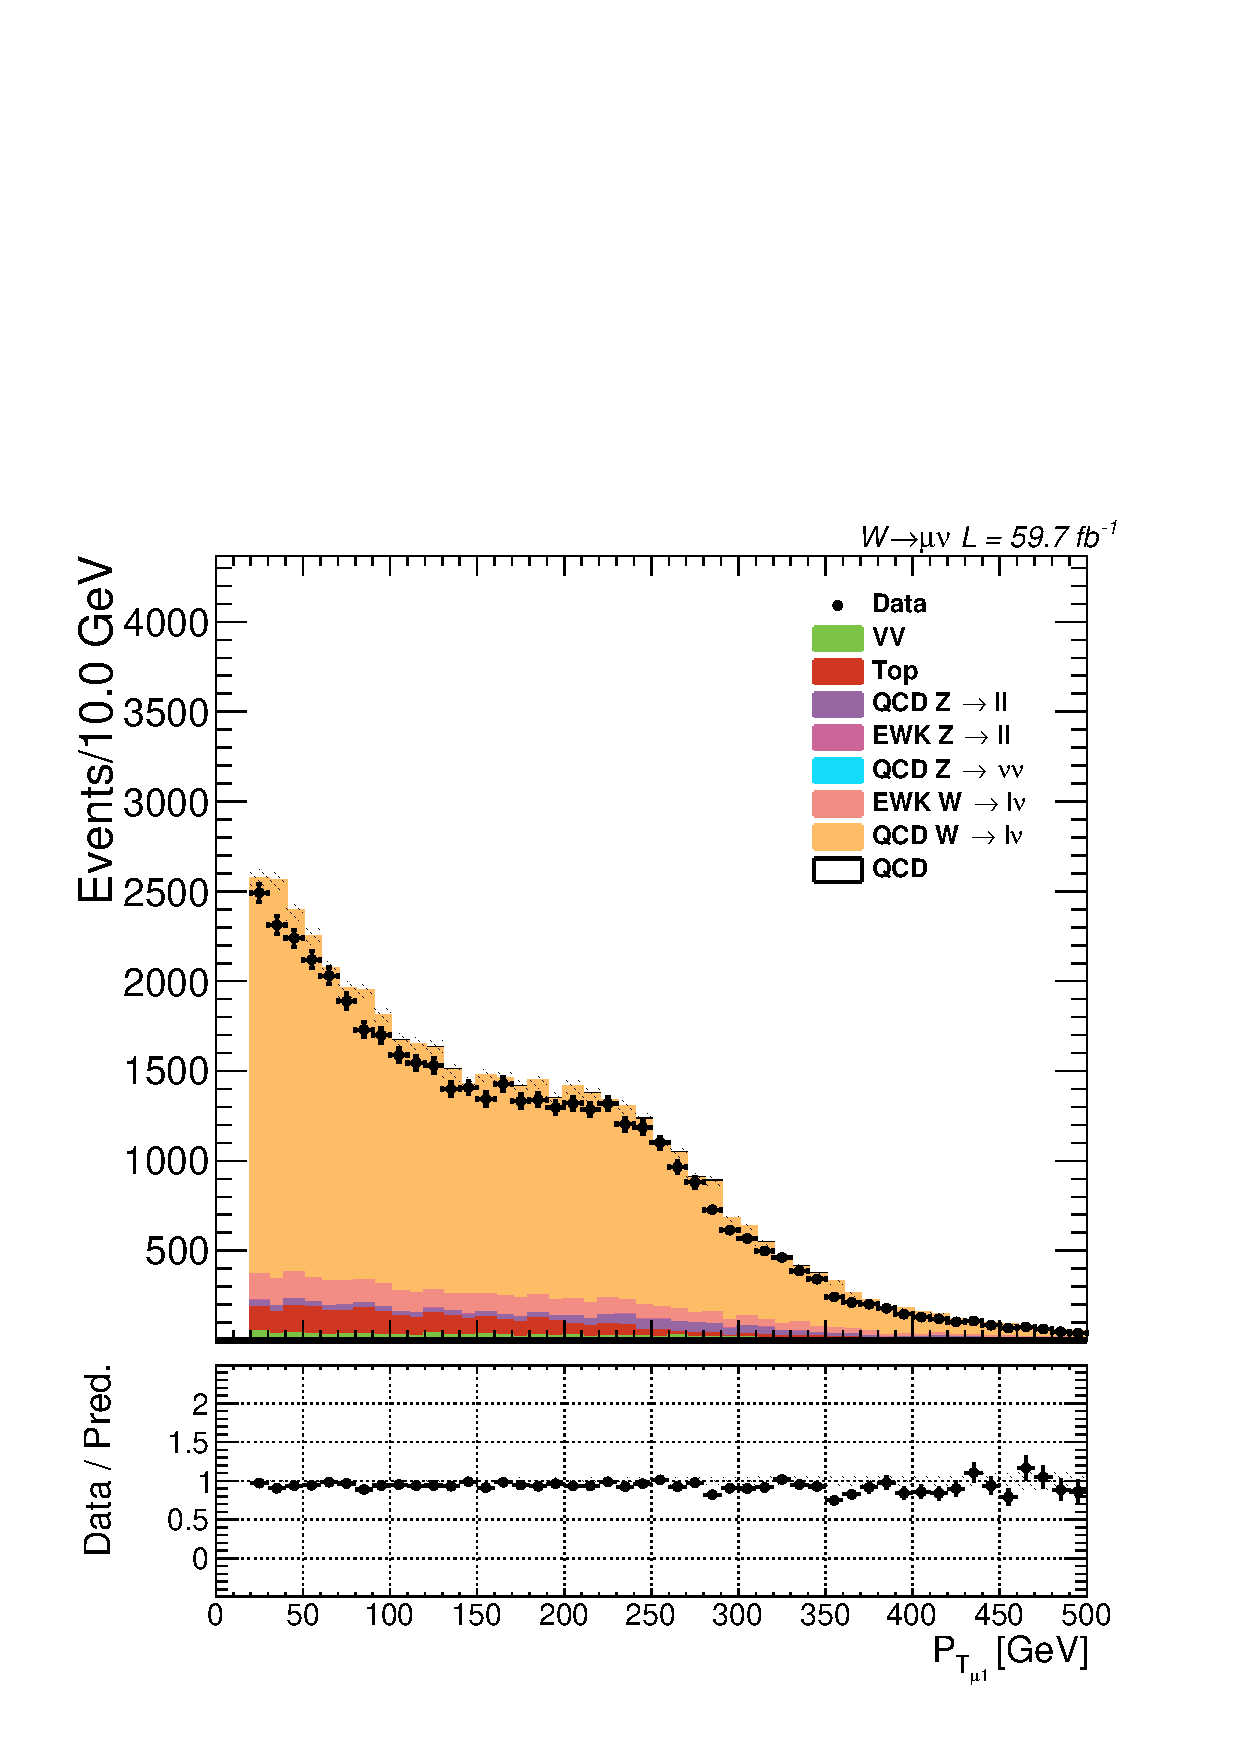
\includegraphics[width=0.49\textwidth]{Control_Regions/2018_MTR/Wmunu/Leading_muon_pt.pdf}
    }
    \subfigure[$\eta_{\mu,1}$ - MTR]{
    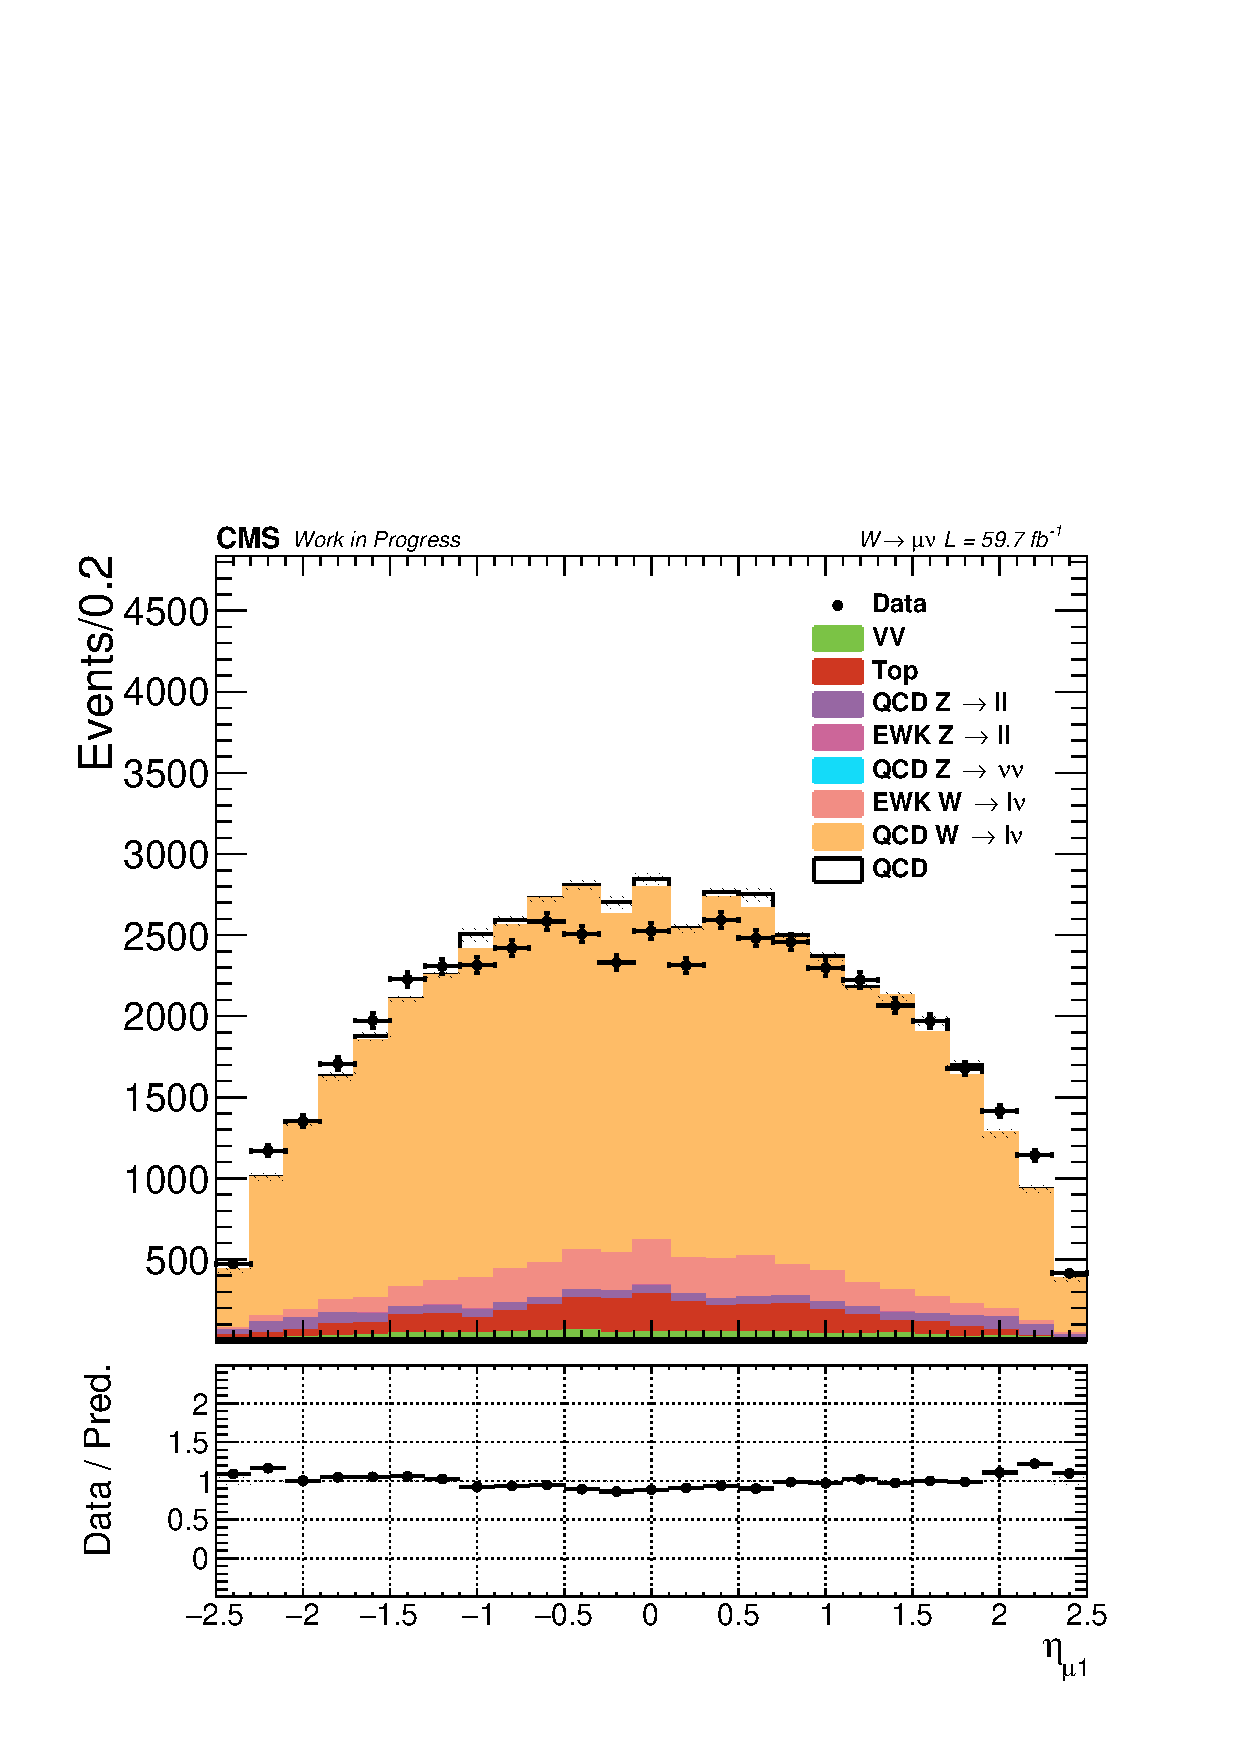
\includegraphics[width=0.49\textwidth]{Control_Regions/2018_MTR/Wmunu/Leading_muon_eta.pdf}
    }\\
    \subfigure[$p_{T_{\mu,1}}$ - VTR]{
    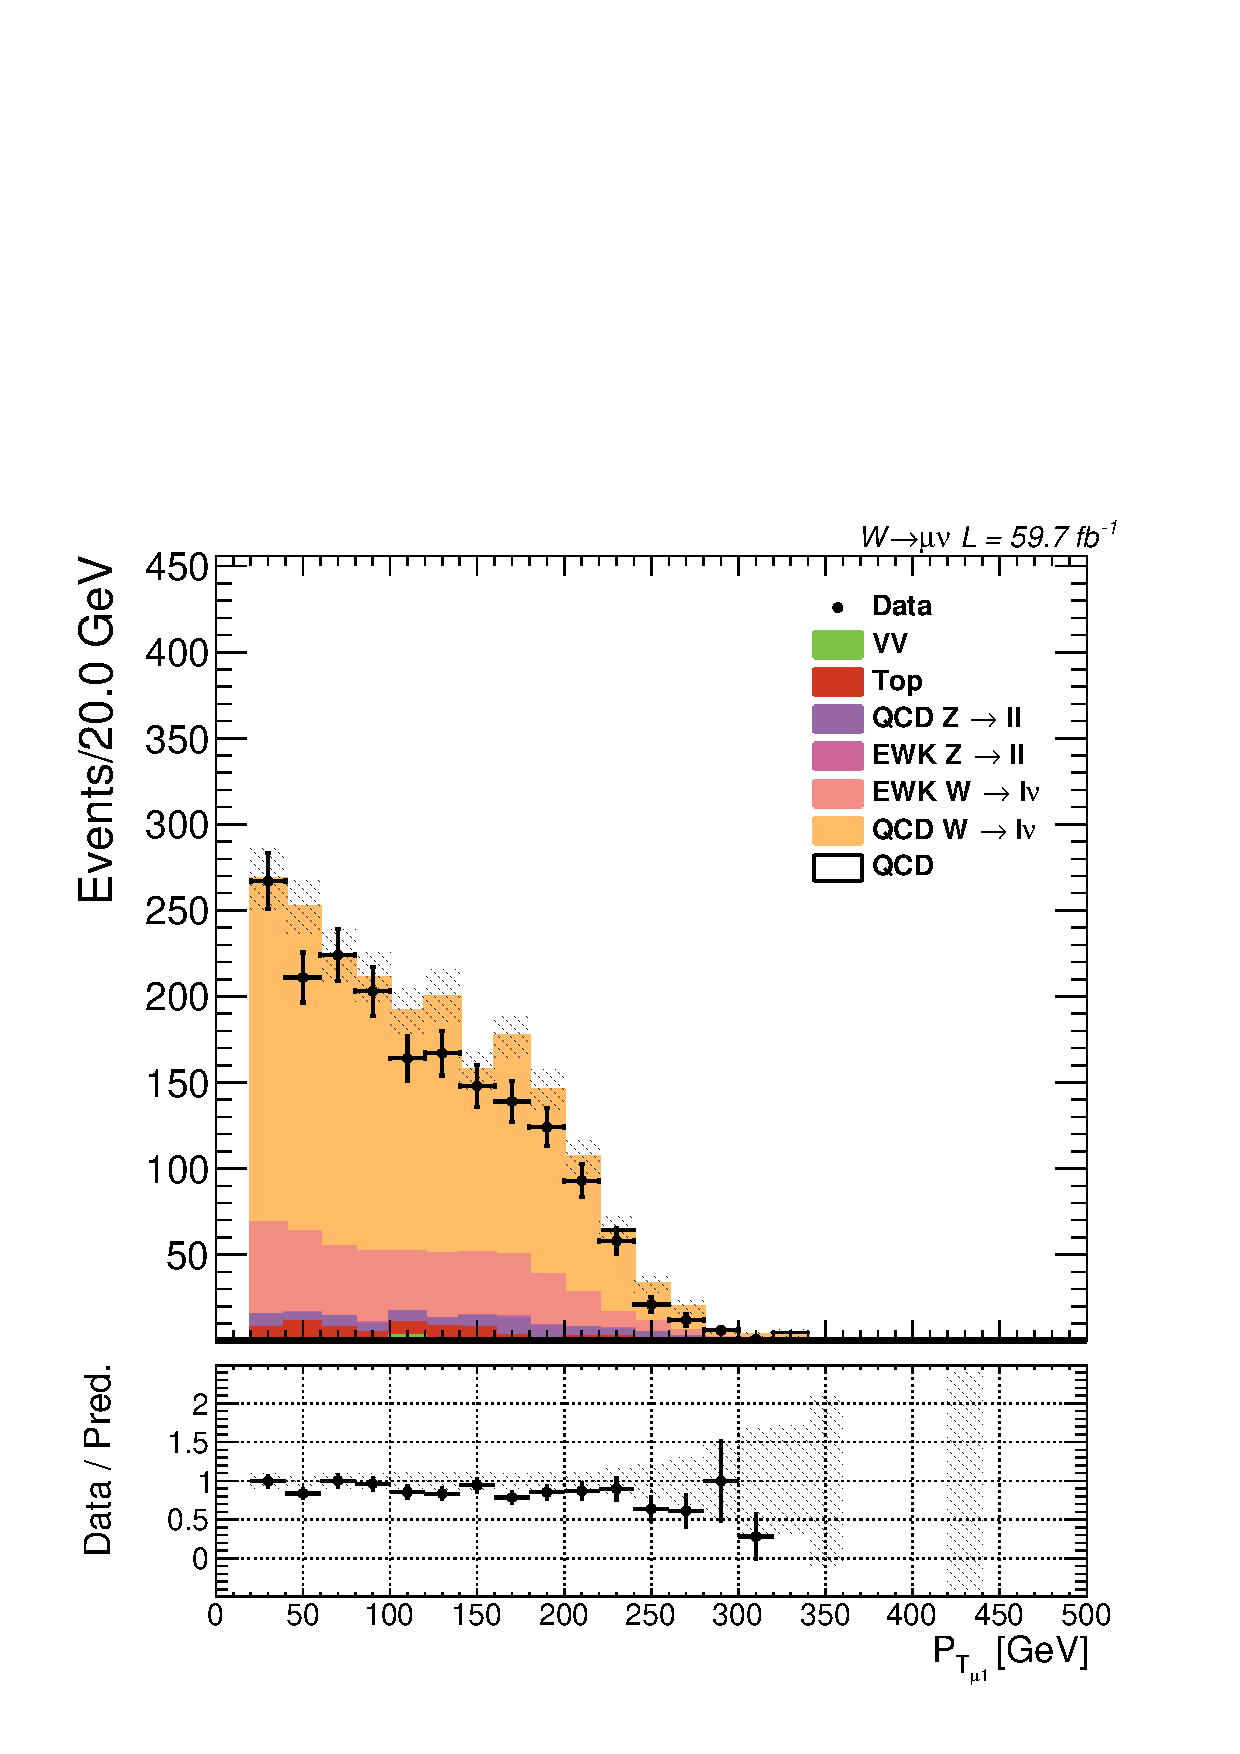
\includegraphics[width=0.49\textwidth]{Control_Regions/2018_VTR/Wmunu/Leading_muon_pt.pdf}
    }
    \subfigure[$\eta_{\mu,1}$  - VTR]{
    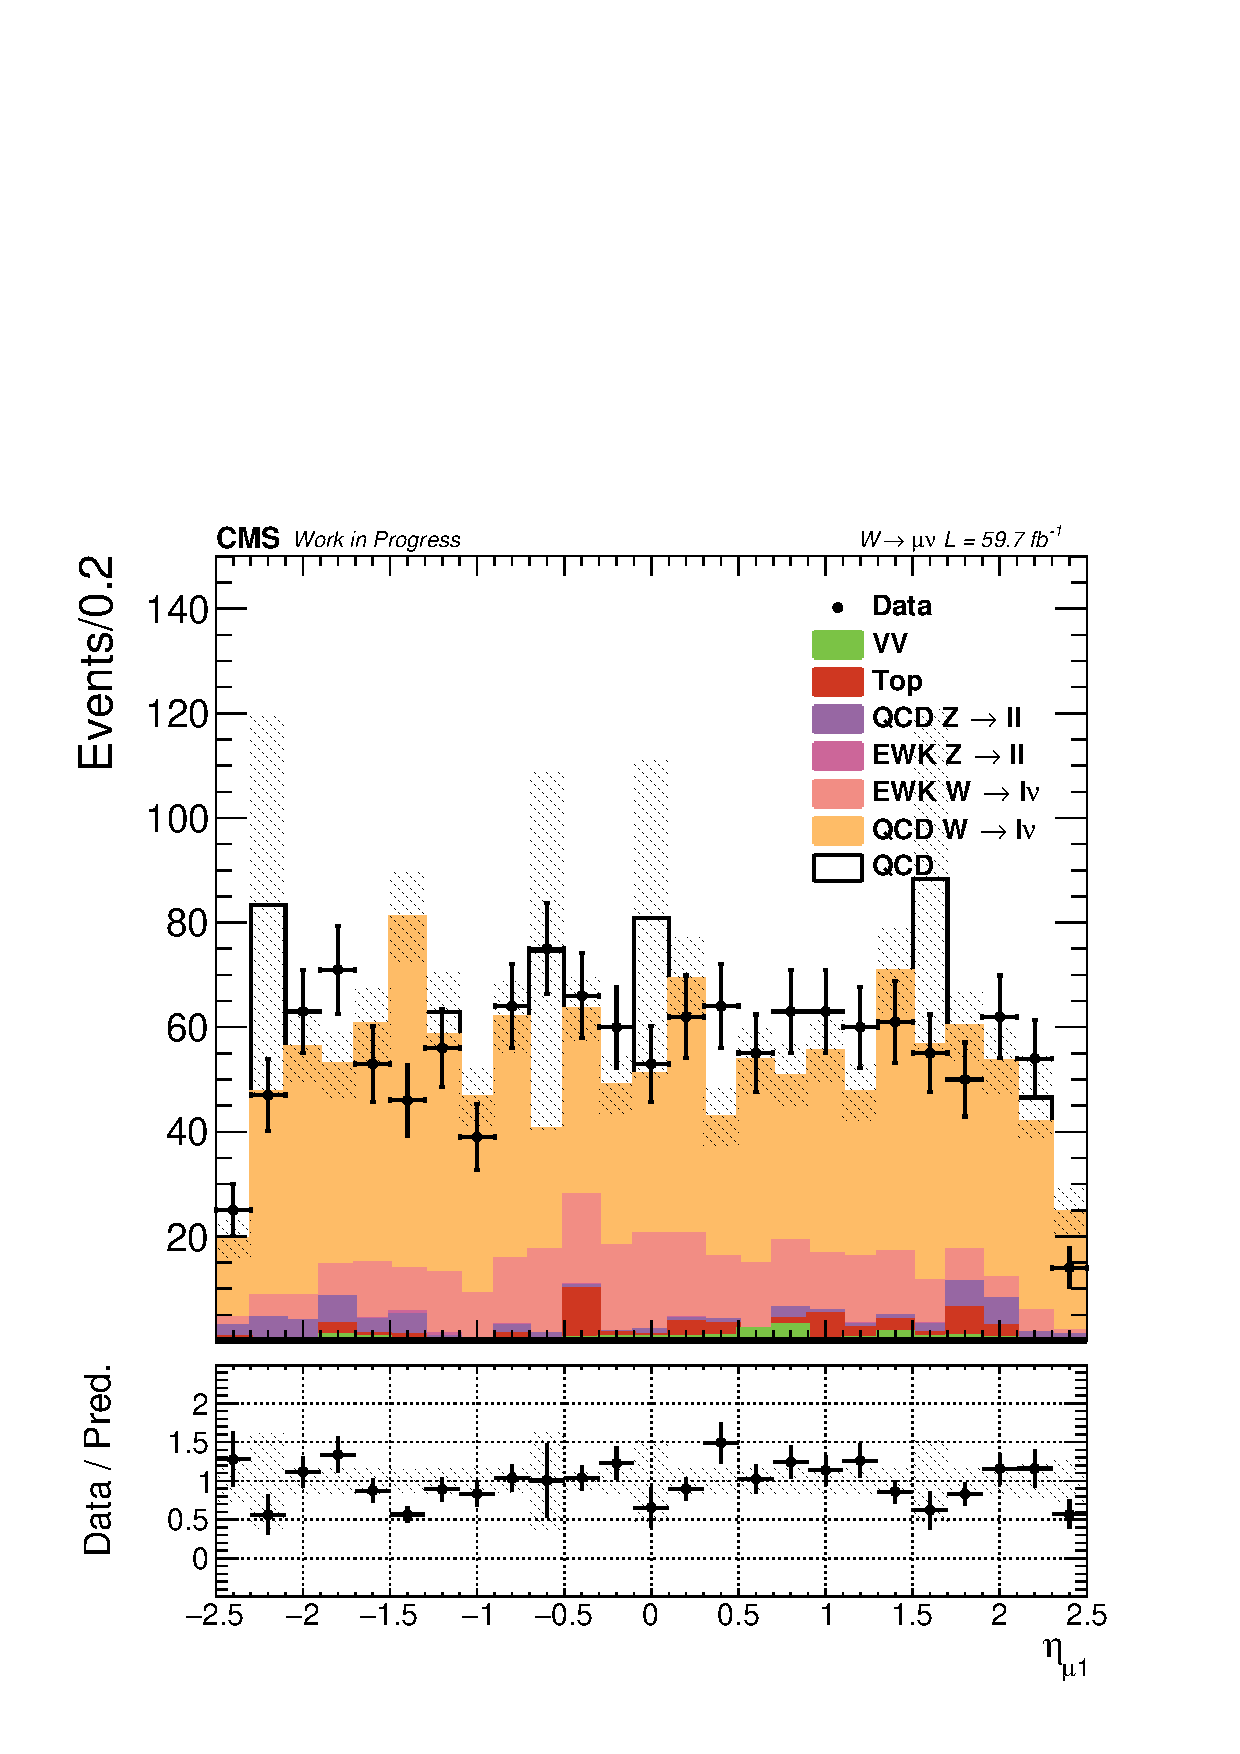
\includegraphics[width=0.49\textwidth]{Control_Regions/2018_VTR/Wmunu/Leading_muon_eta.pdf}
    }
  \caption{Distributions of $p_{T_{\mu,1}}$and $\eta_{\mu,1}$ variables in the single muon region for MTR (top) and VTR (bottom) categories for the 2018 era of data taking.}
  \label{app:2018_Wmunu_1}
\end{figure}
%%%%%%%%%%%%%%%%%%%%ELECTRON REGIONS%%%%%%%%%%%%%%%%%%%%%%%%%%%%%%%%%%%%%%%%%%%%




\begin{figure}[htbp]
  \centering
    \subfigure[$p_{T_{e,1}}$ - MTR]{
    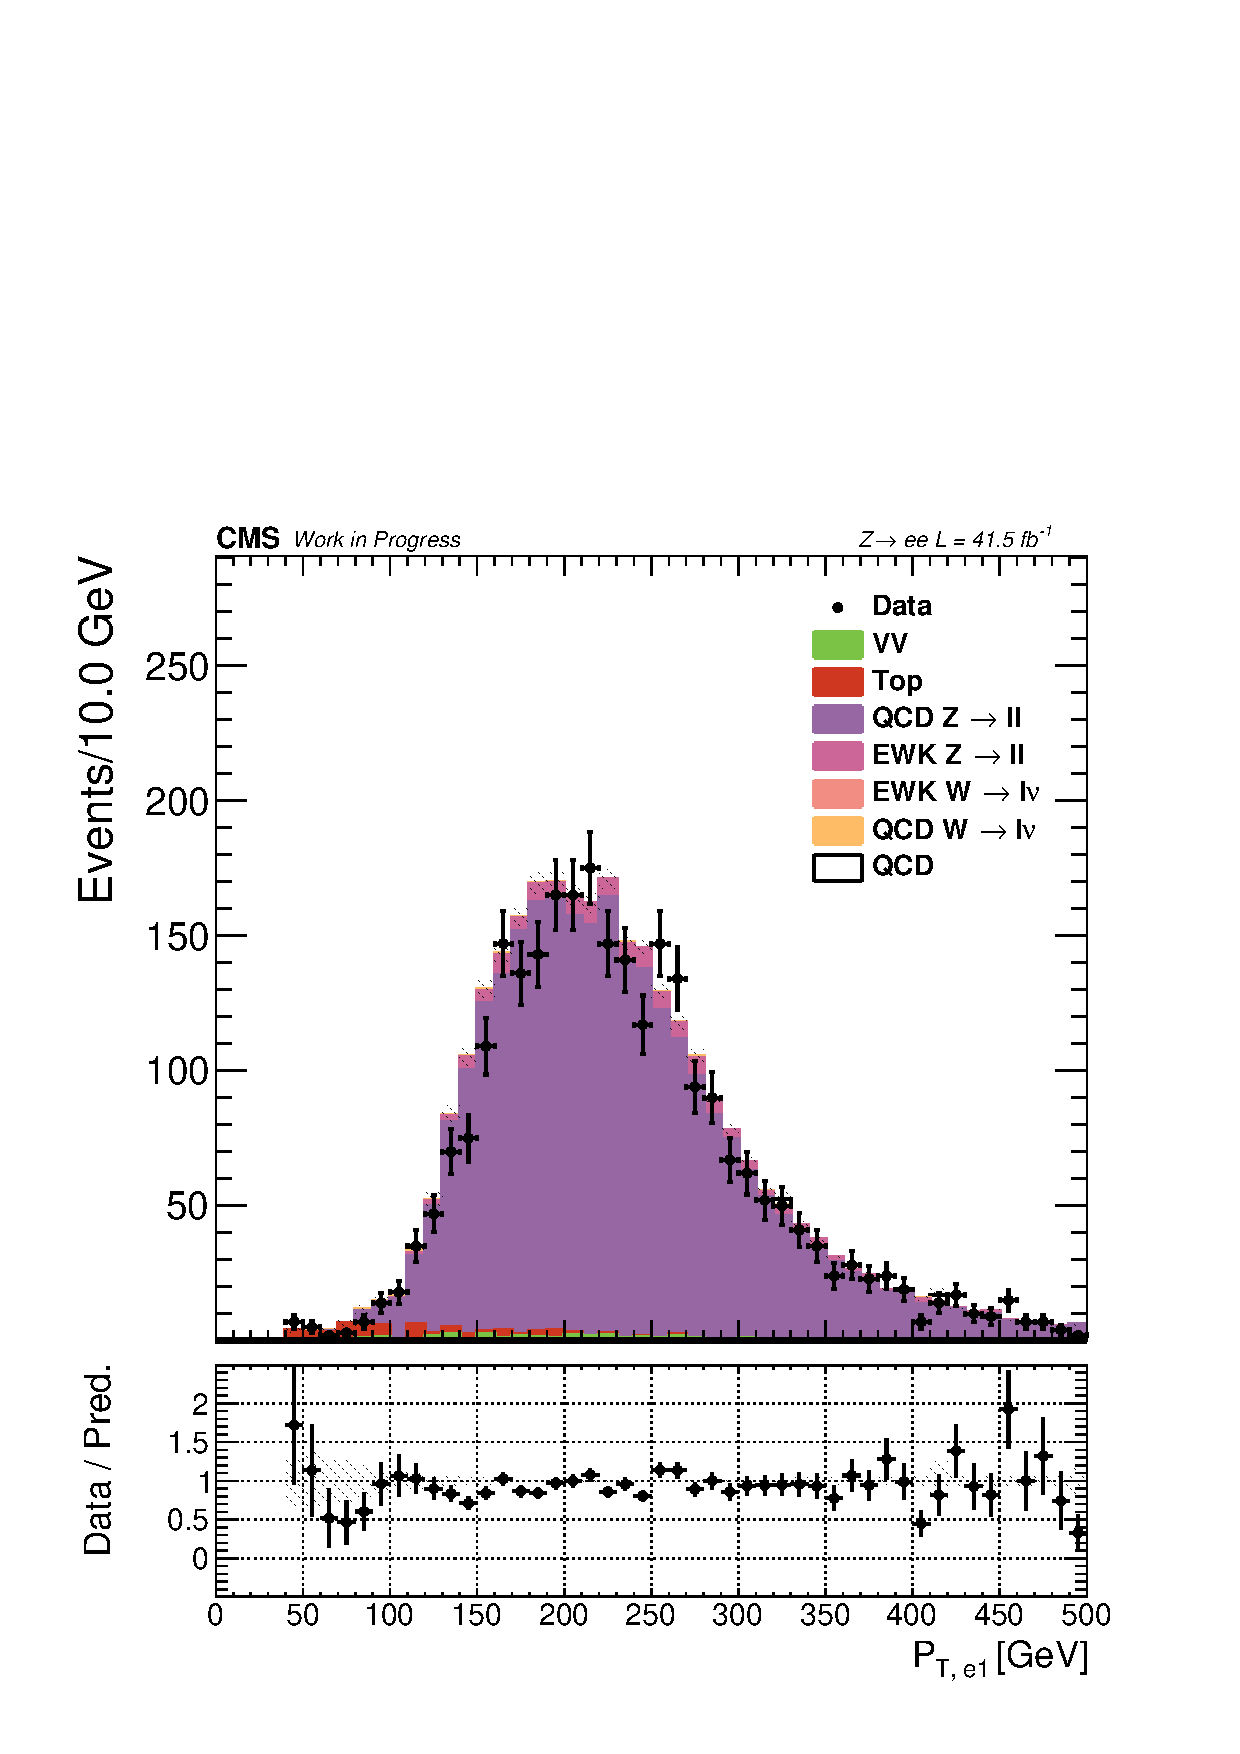
\includegraphics[width=0.49\textwidth]{Control_Regions/2017_MTR/Zee/Leading_electron_pt.pdf}
    }
    \subfigure[$\eta_{e,1}$ - MTR]{
    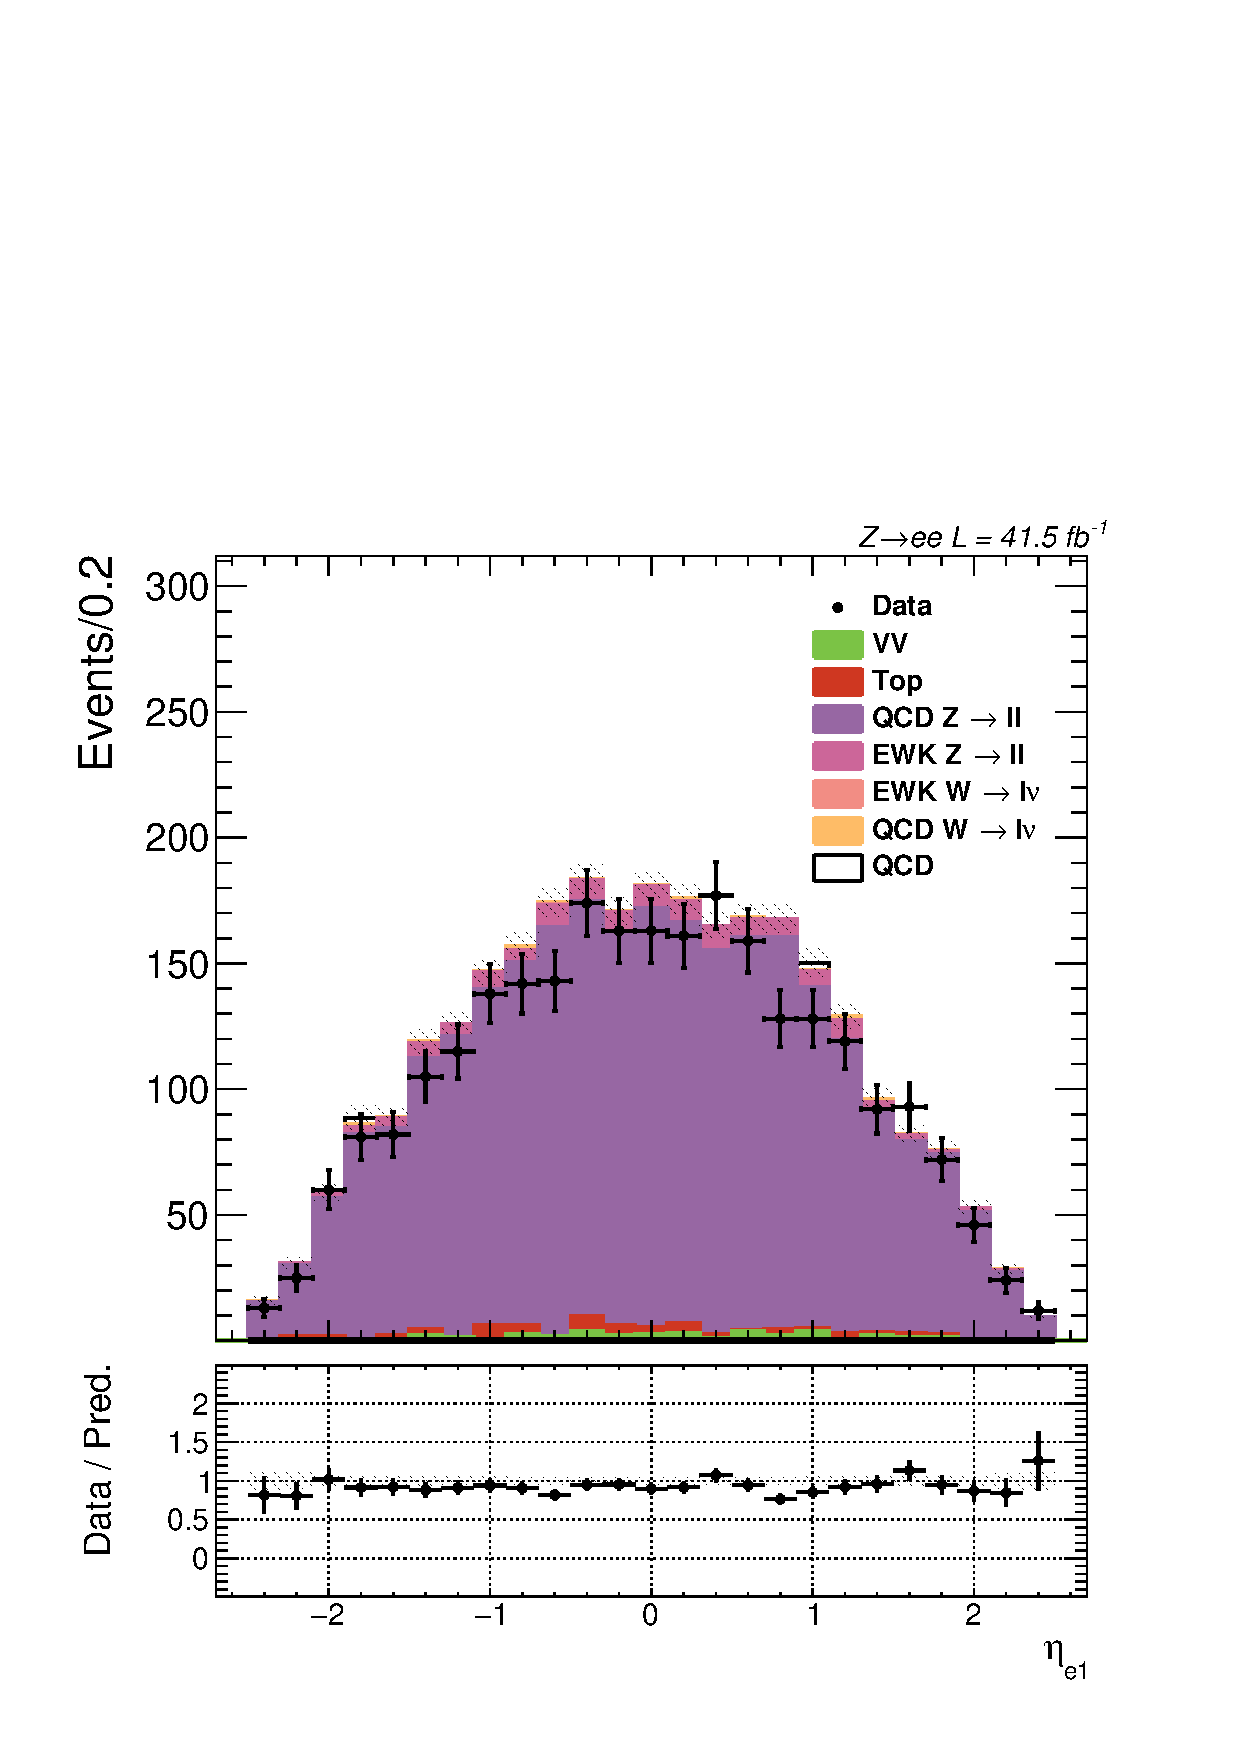
\includegraphics[width=0.49\textwidth]{Control_Regions/2017_MTR/Zee/Leading_electron_eta.pdf}
    }\\
    \subfigure[$p_{T_{e,1}}$ - VTR]{
    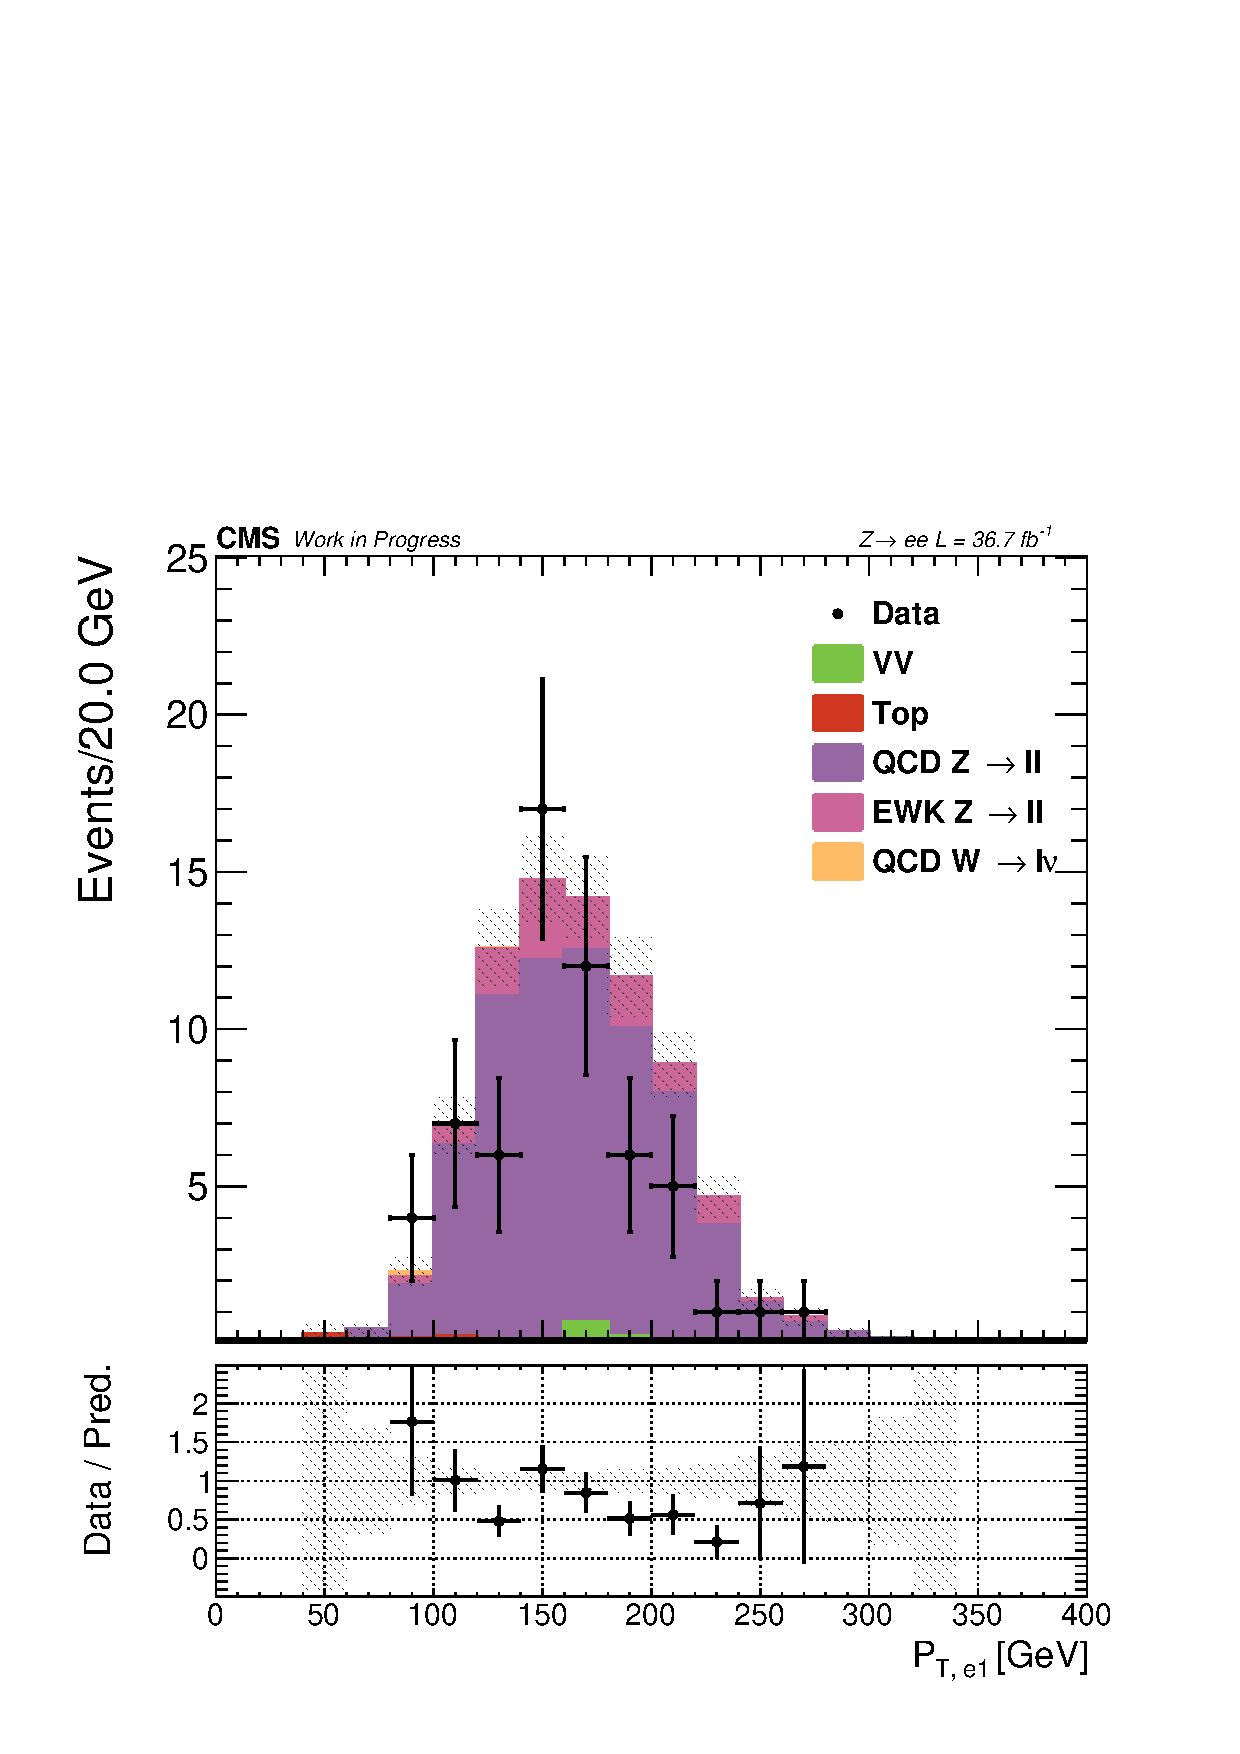
\includegraphics[width=0.49\textwidth]{Control_Regions/2017_VTR/Zee/Leading_electron_pt.pdf}
    }
    \subfigure[$\eta_{e,1}$  - VTR]{
    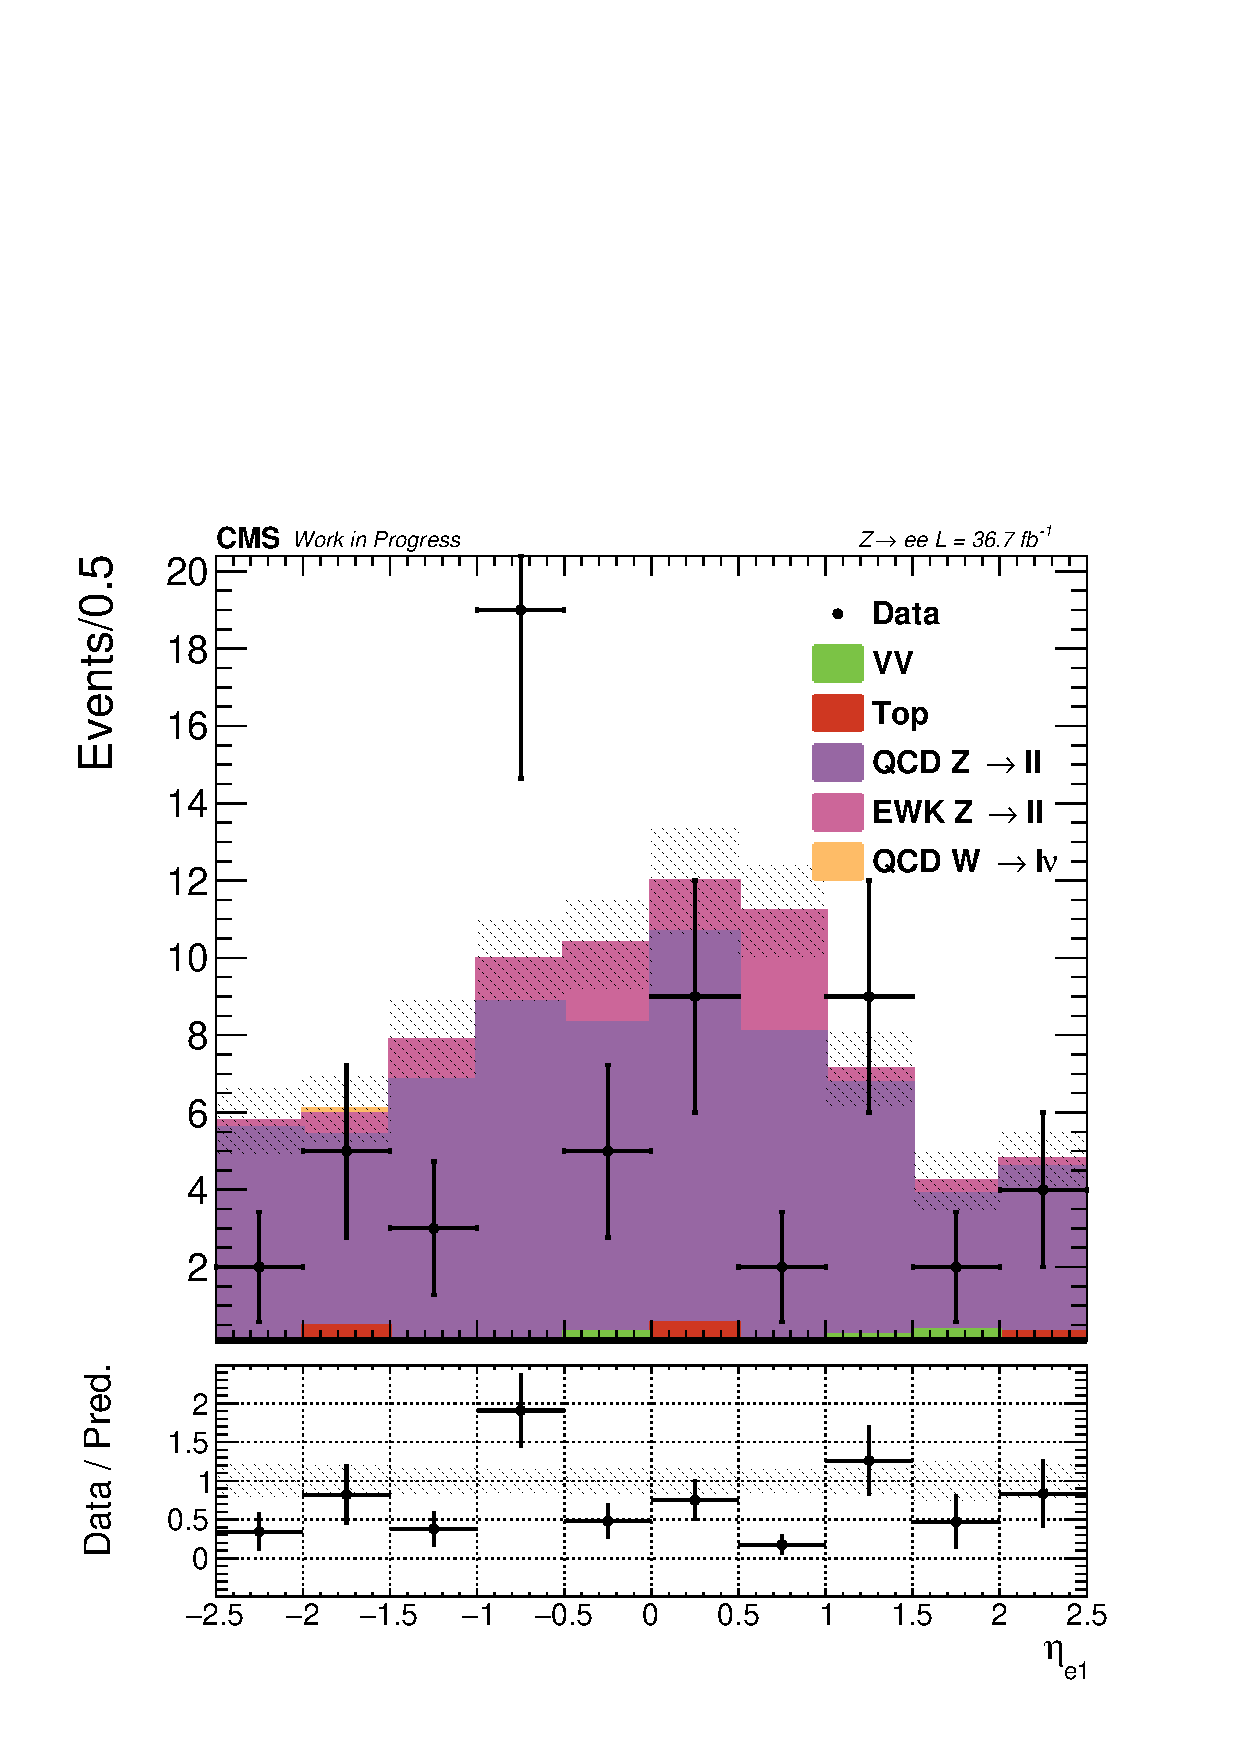
\includegraphics[width=0.49\textwidth]{Control_Regions/2017_VTR/Zee/Leading_electron_eta.pdf}
    }
  \caption{Distributions of $p_{T_{e,1}}$ and $\eta_{e,1}$ variables in the double electron region for MTR (top) and VTR (bottom) categories for the 2017 era of data taking.}
  \label{app:2017_Zee_1}
\end{figure}

\begin{figure}[htbp]
  \centering
    \subfigure[$p_{T_{e,1}}$ - MTR]{
    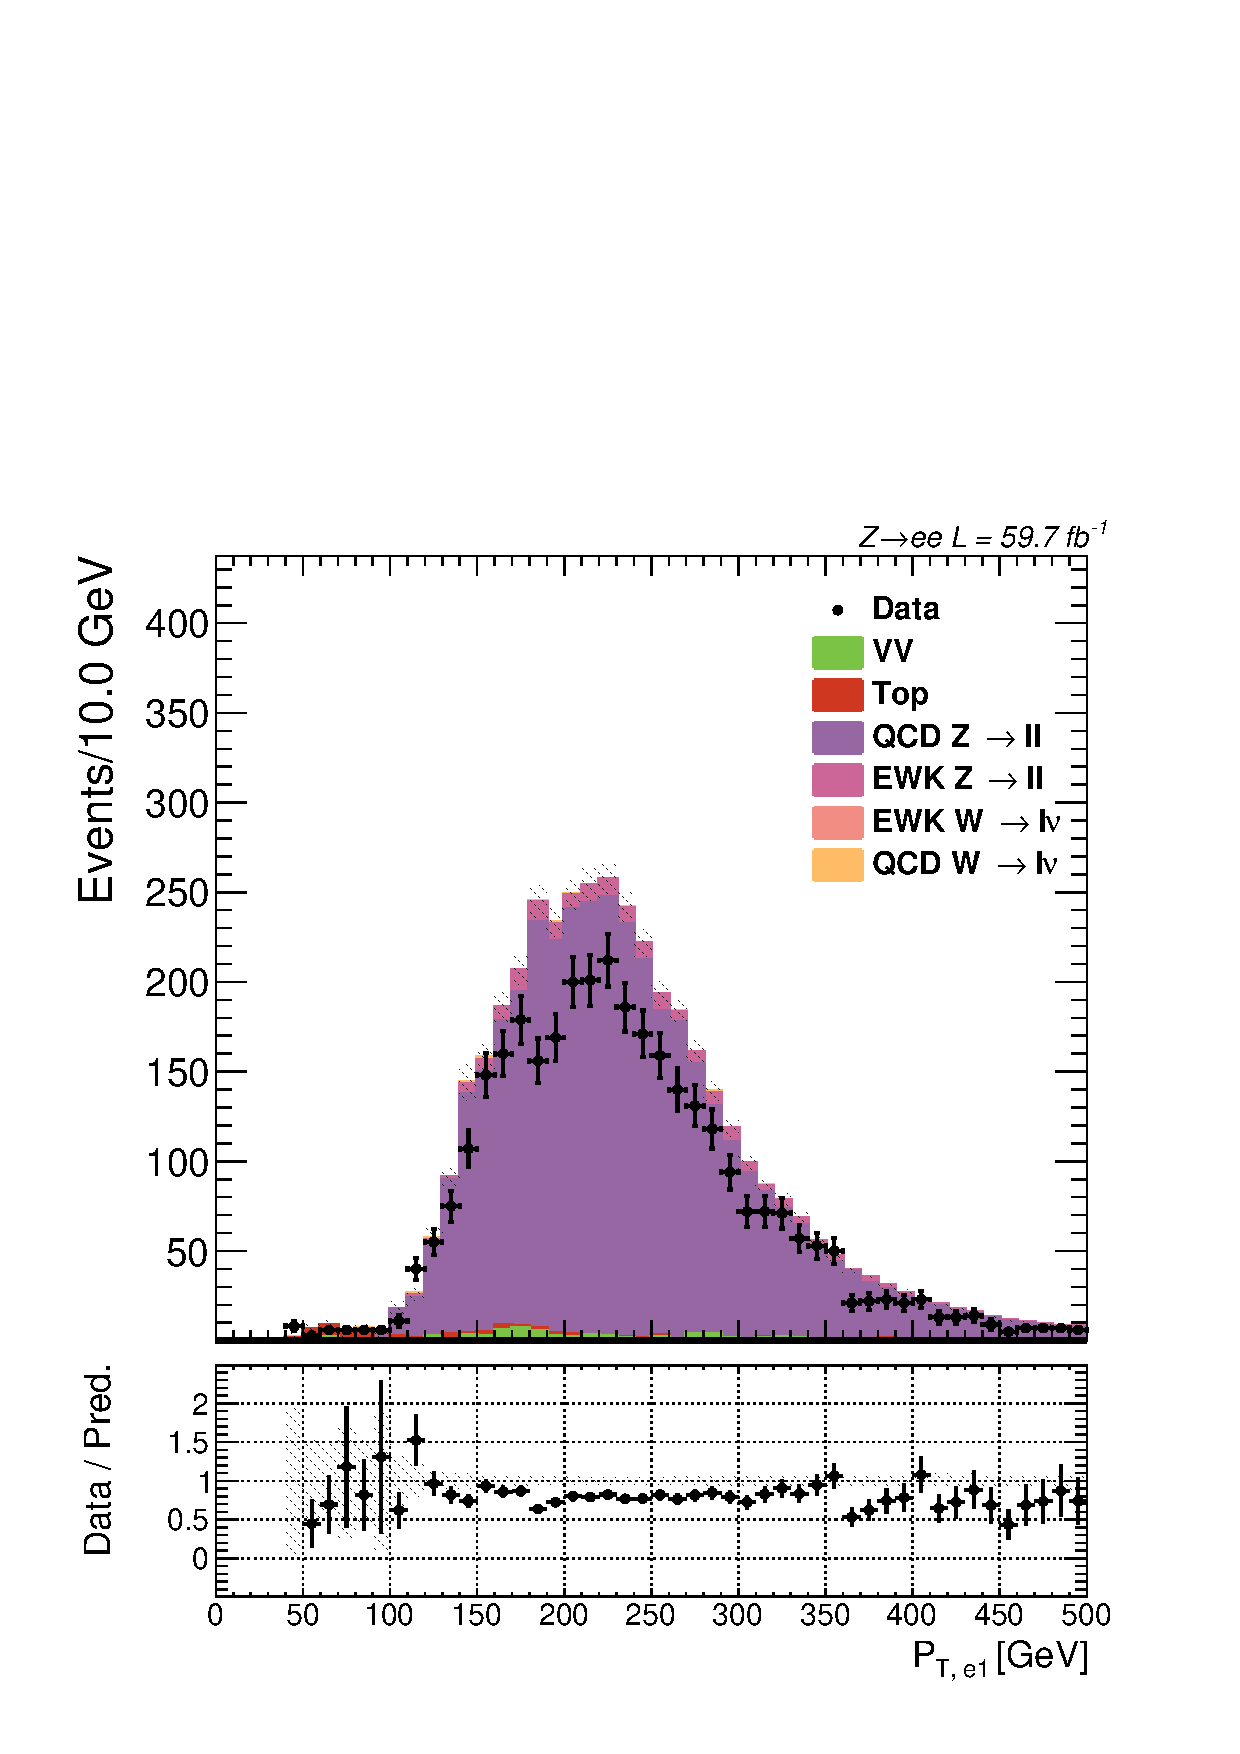
\includegraphics[width=0.49\textwidth]{Control_Regions/2018_MTR/Zee/Leading_electron_pt.pdf}
    }
    \subfigure[$\eta_{e,1}$ - MTR]{
    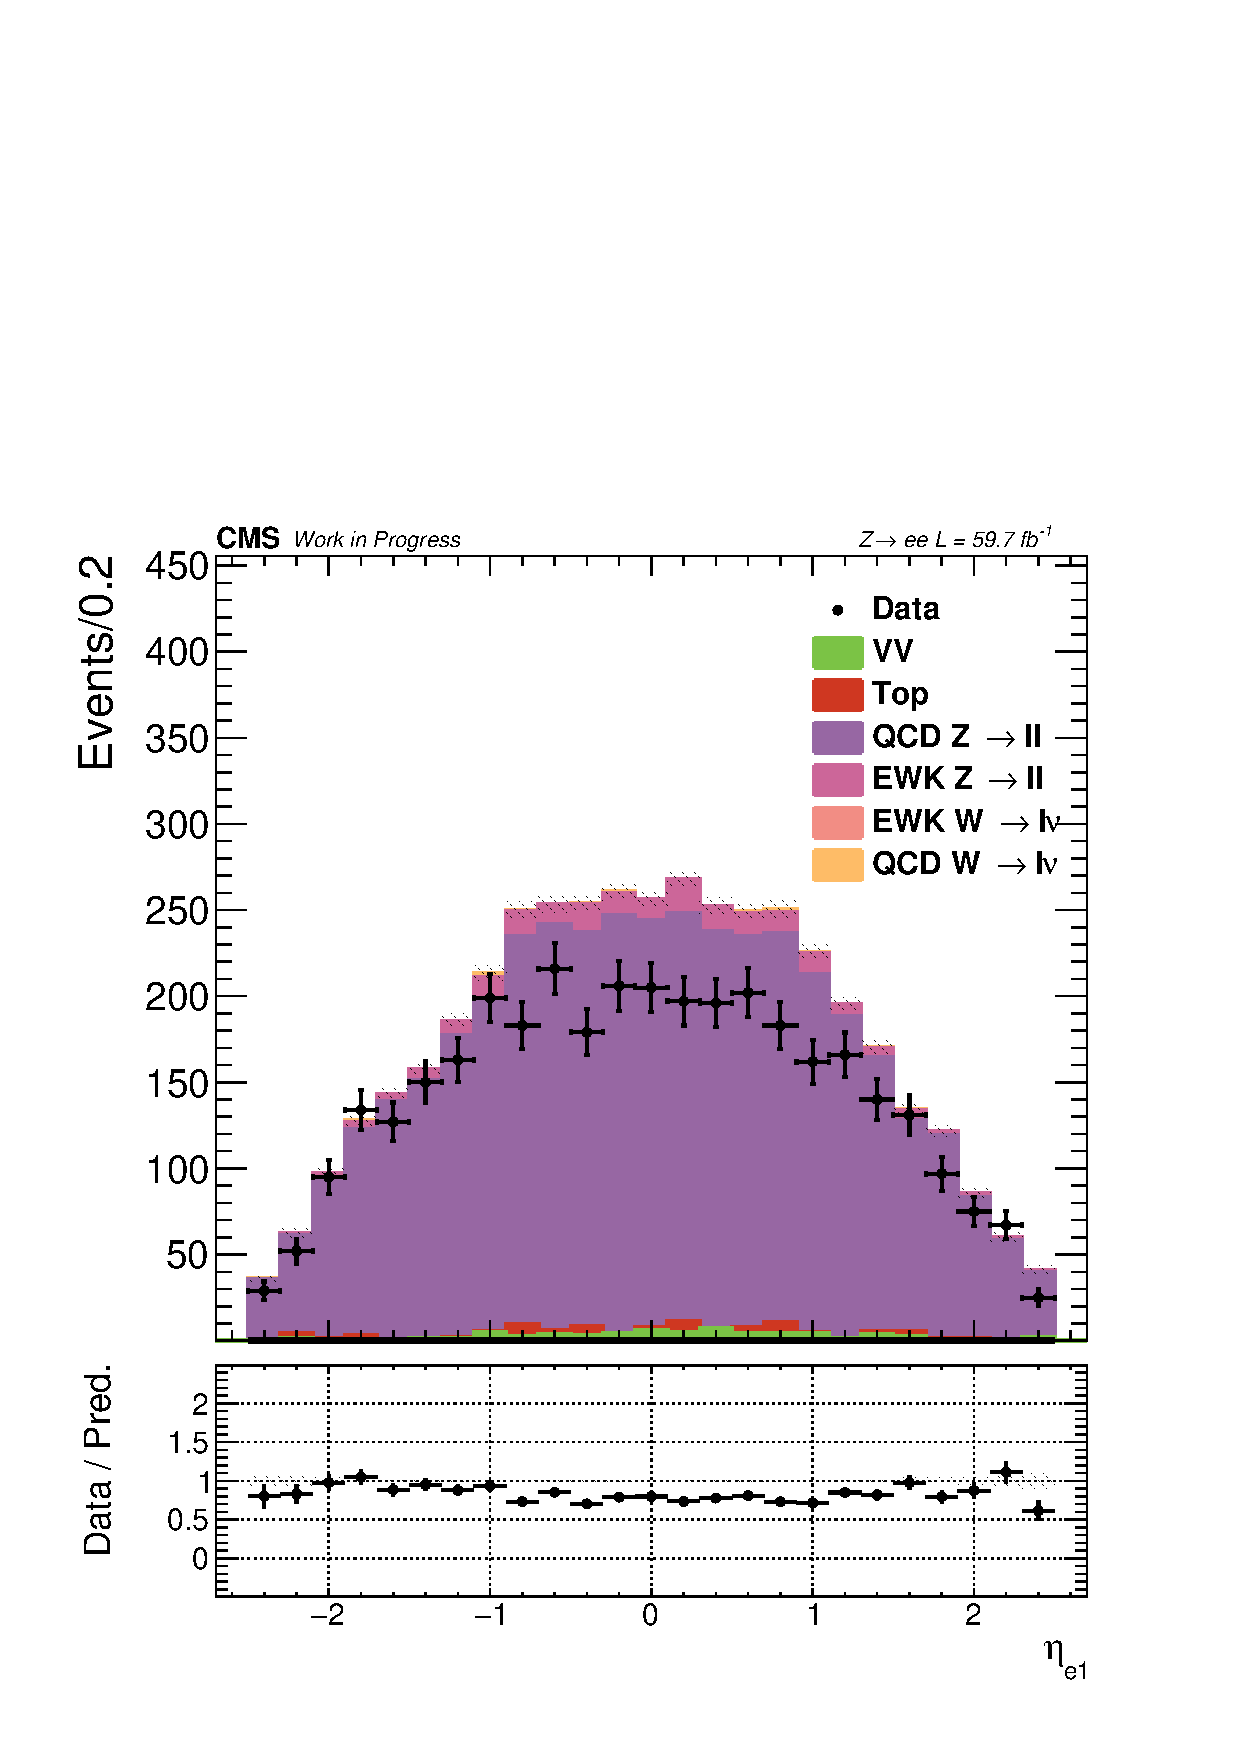
\includegraphics[width=0.49\textwidth]{Control_Regions/2018_MTR/Zee/Leading_electron_eta.pdf}
    }\\
    \subfigure[$p_{T_{e,1}}$ - VTR]{
    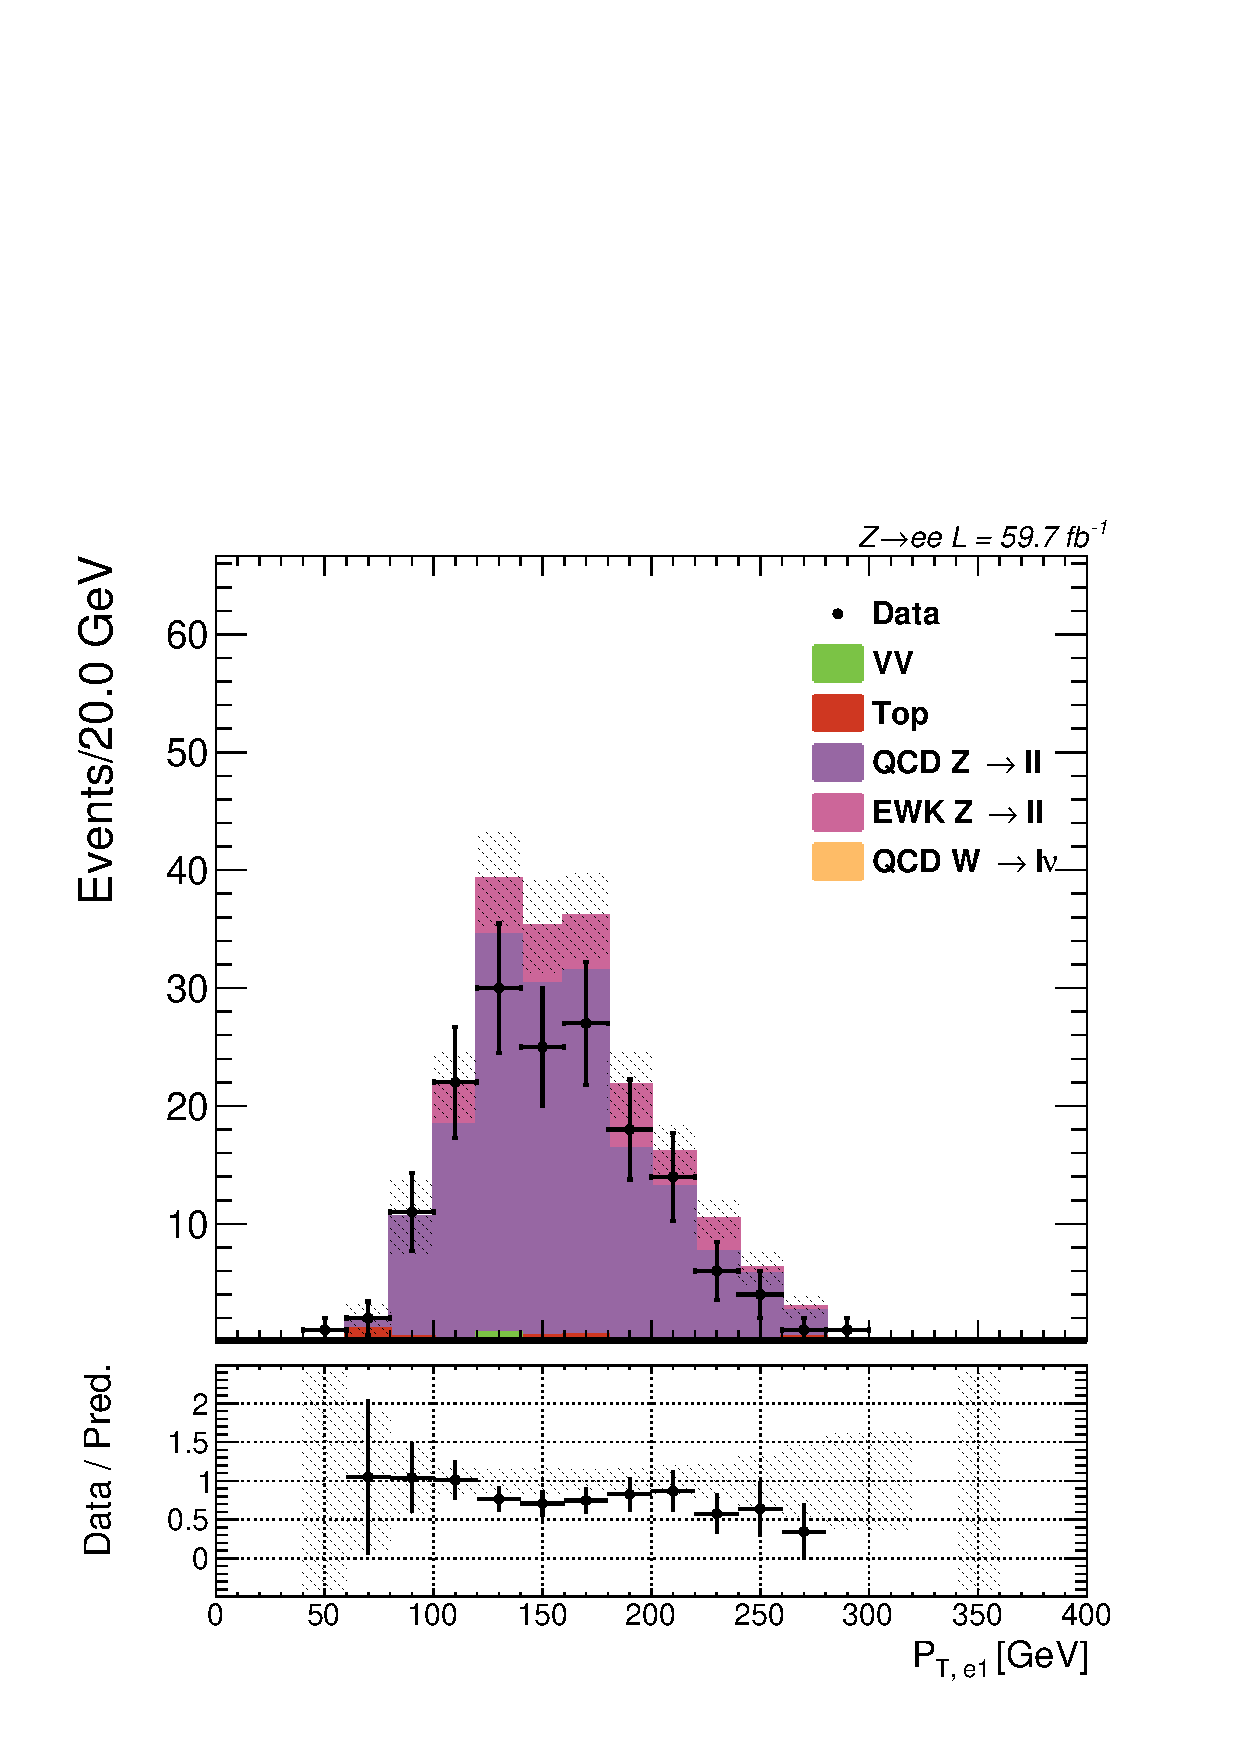
\includegraphics[width=0.49\textwidth]{Control_Regions/2018_VTR/Zee/Leading_electron_pt.pdf}
    }
    \subfigure[$\eta_{e,1}$  - VTR]{
    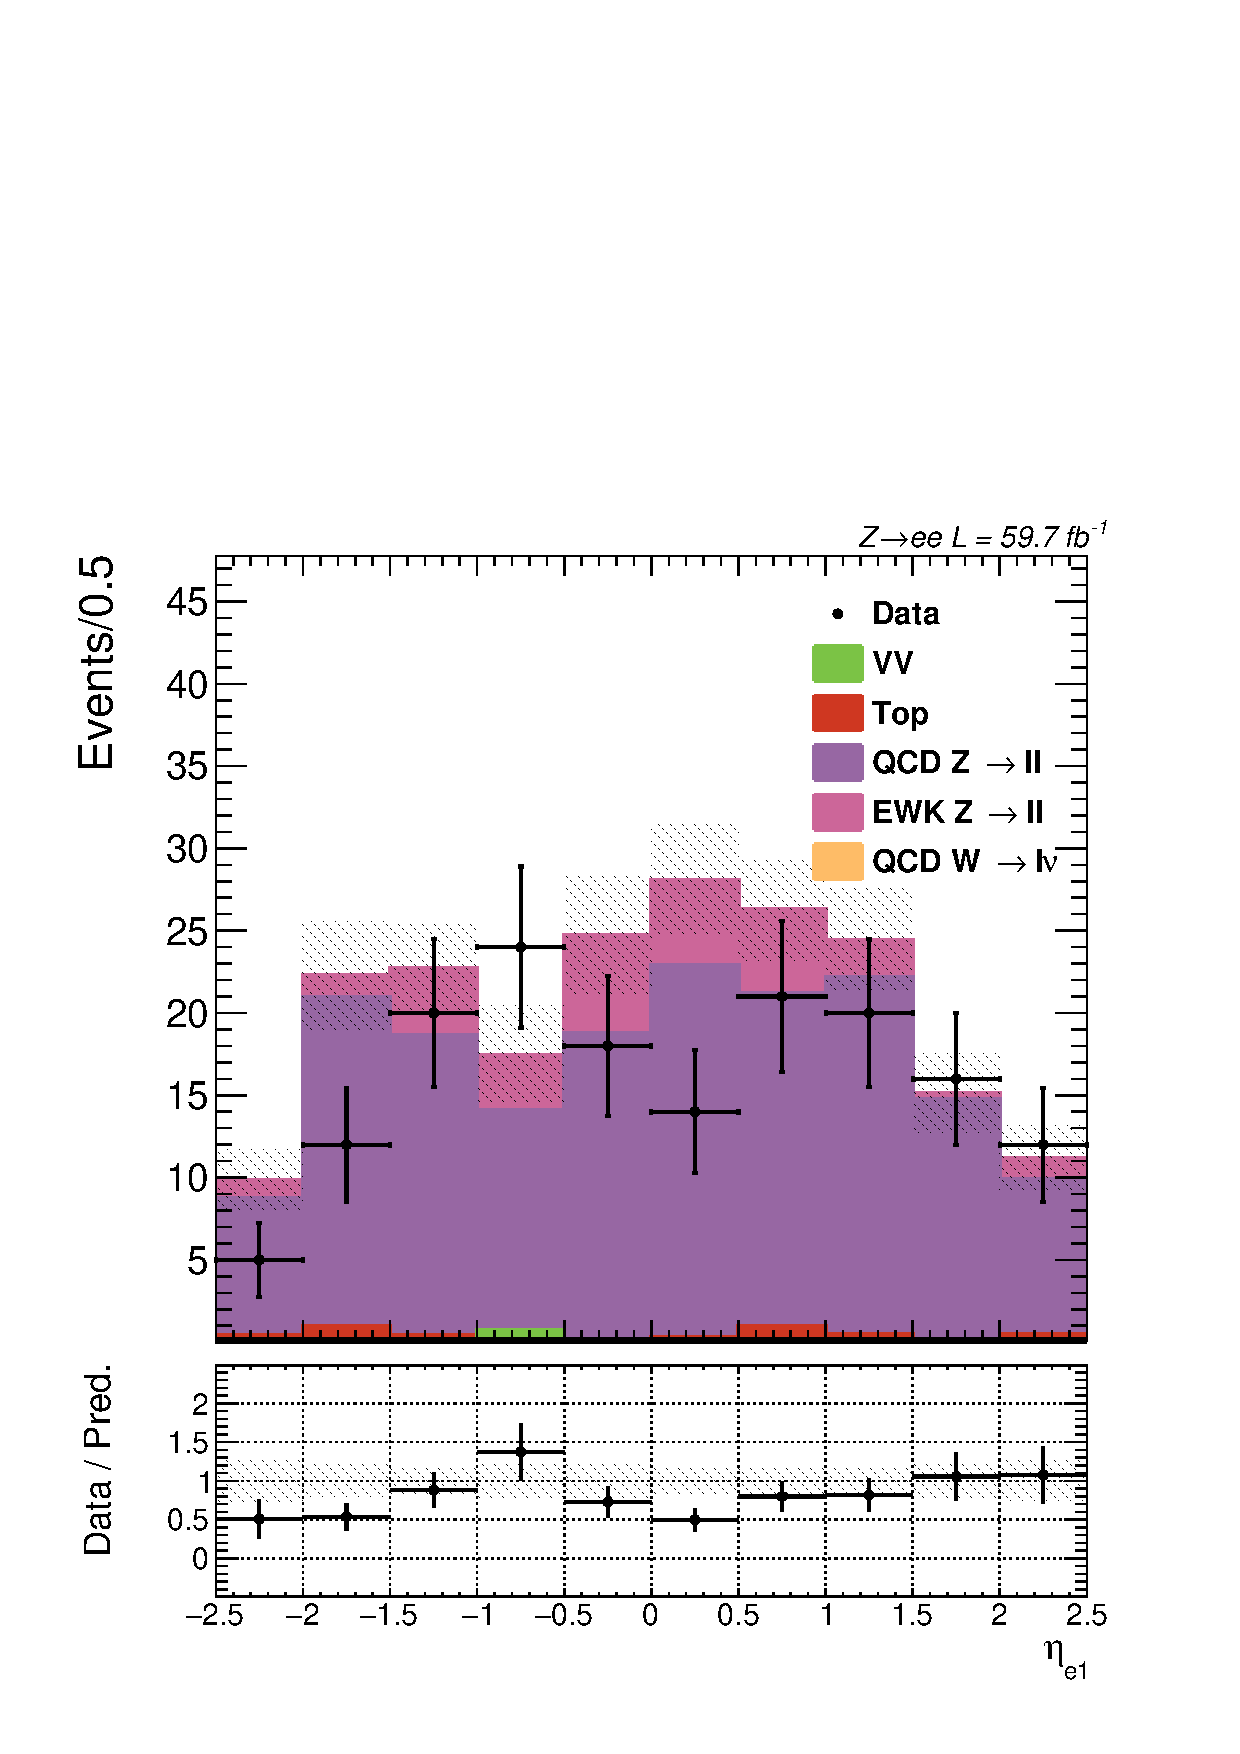
\includegraphics[width=0.49\textwidth]{Control_Regions/2018_VTR/Zee/Leading_electron_eta.pdf}
    }
  \caption{Distributions of $p_{T_{e,1}}$ and $\eta_{e,1}$ variables in the double electron region for MTR (top) and VTR (bottom) categories for the 2018 era of data taking.}
  \label{app:2018_Zee_1}
\end{figure}

\begin{figure}[htbp]
  \centering
    \subfigure[$p_{T_{e,1}}$ - VTR]{
    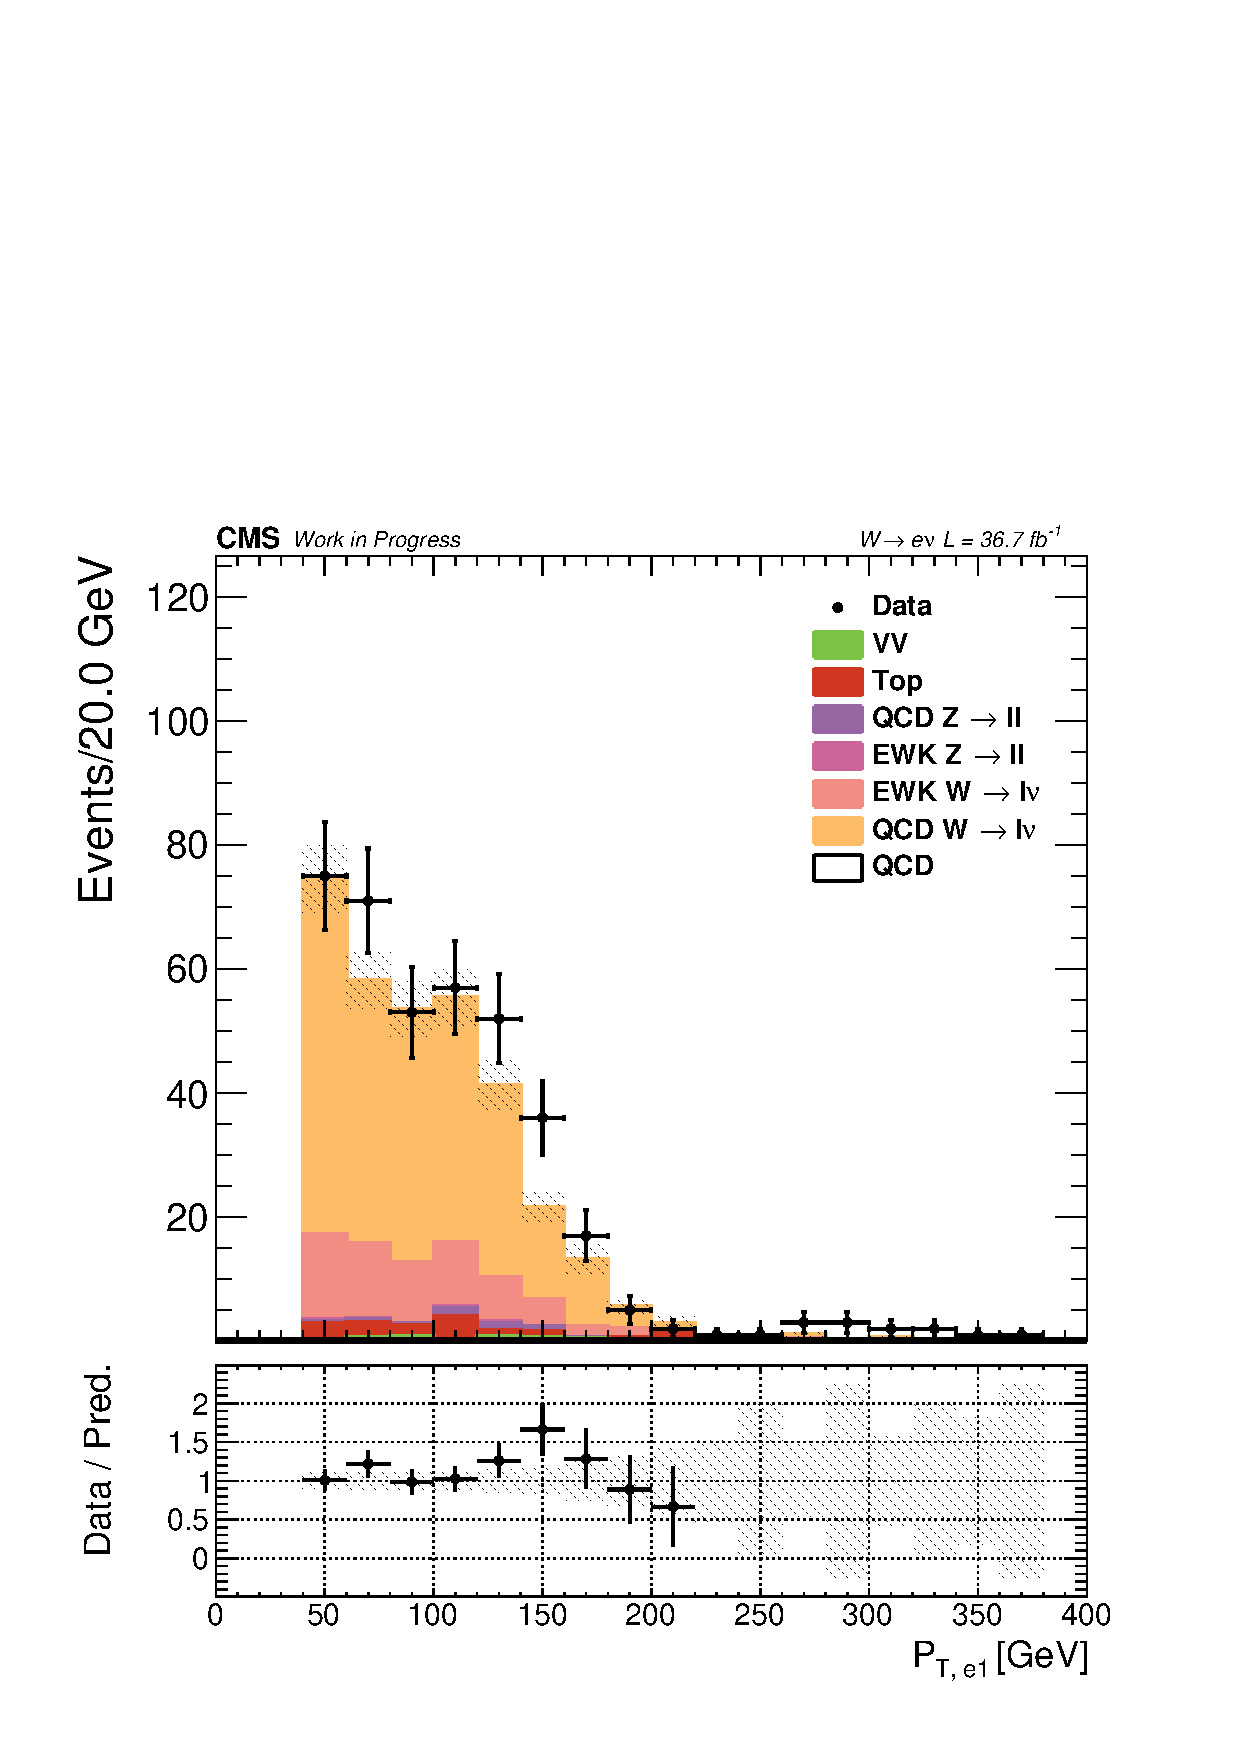
\includegraphics[width=0.49\textwidth]{Control_Regions/2017_VTR/Wenu/Leading_electron_pt.pdf}
    }\\
    \subfigure[$\eta_{e,1}$  - VTR]{
    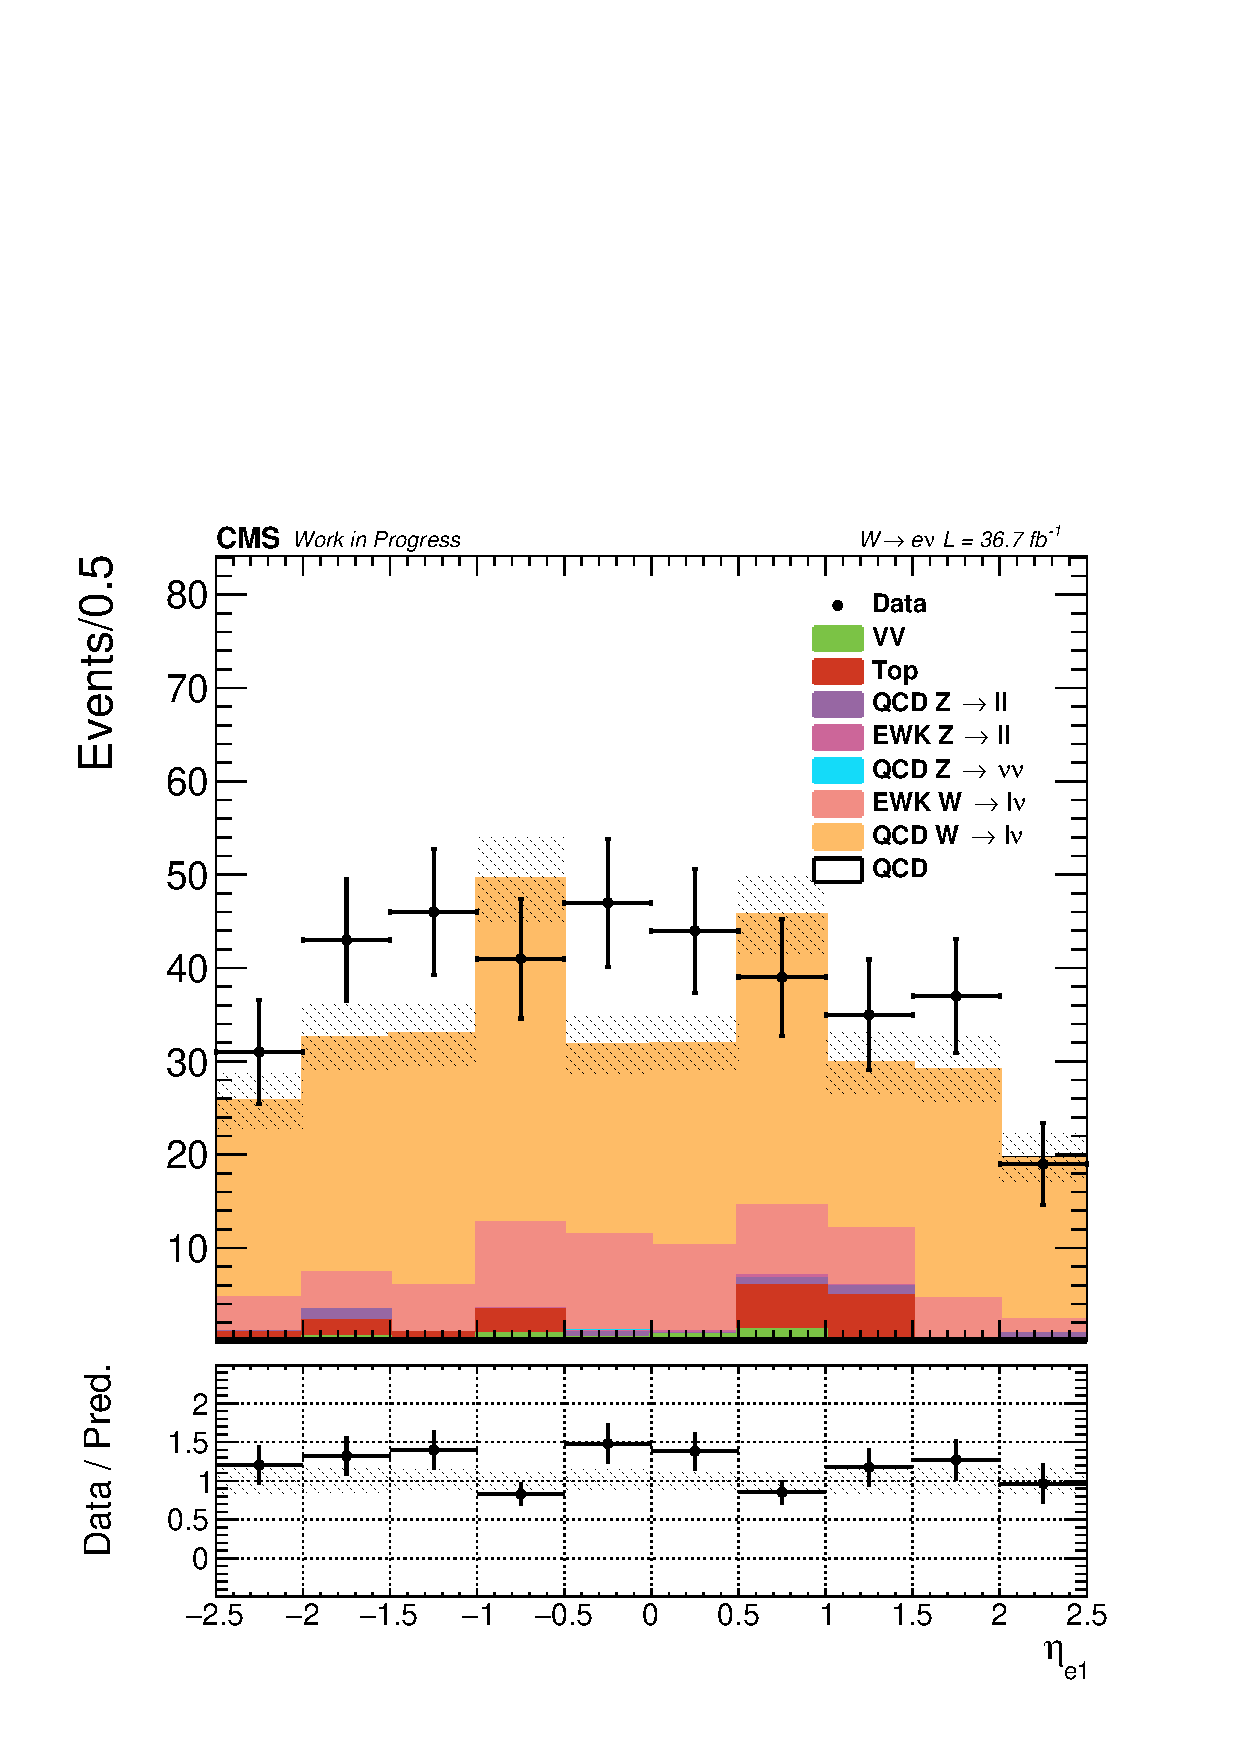
\includegraphics[width=0.49\textwidth]{Control_Regions/2017_VTR/Wenu/Leading_electron_eta.pdf}
    }
  \caption{Distributions of $p_{T_{e,1}}$ and $\eta_{e,1}$ variables in the single electron region for the VTR category for the 2017 era of data taking.}
  \label{app:2017_Wenu_1}
\end{figure}
\newpage

\begin{figure}[htbp]
  \centering
    \subfigure[$p_{T_{e,1}}$ - MTR]{
    \includegraphics[width=0.49\textwidth]{Control_Regions/2018_MTR/Wenu/Leading_electron_pt.pdf}
    }
    \subfigure[$\eta_{e,1}$ - MTR]{
    \includegraphics[width=0.49\textwidth]{Control_Regions/2018_MTR/Wenu/Leading_electron_eta.pdf}
    }\\
    \subfigure[$p_{T_{e,1}}$ - VTR]{
    \includegraphics[width=0.49\textwidth]{Control_Regions/2018_VTR/Wenu/Leading_electron_pt.pdf}
    }
    \subfigure[$\eta_{e,1}$  - VTR]{
    \includegraphics[width=0.49\textwidth]{Control_Regions/2018_VTR/Wenu/Leading_electron_eta.pdf}
    }
  \caption{Distributions of $p_{T_{e,1}}$ and $\eta_{e,1}$ variables in the single electron region for MTR (top) and VTR (bottom) categories for the 2018 era of data taking.}
  \label{app:2018_Wenu_1}
\end{figure}



\newpage

\section{Fit structure and results - supplementary material}



\begin{figure}[htbp]
  \centering
   \includegraphics[width= 0.8\textwidth]{FIt_structure/theory_uncert_VTR_2017.pdf}
    
  \caption{Theoretical uncertainties on $f(\boldsymbol{\theta})$ ratios for the VTR category and 2017 data, presented as a function of $m_{jj}$ for the QCD production modes.}
  \label{app:theory_VTR_2017}
\end{figure}



\newpage



\begin{figure}[htbp]
  \centering
   \subfigure[Dimuon CR]{ \includegraphics[width= 0.47\textwidth]{Results/CRonlyFit/MTR_2017_ZMUMU.pdf}}
     \subfigure[Dielectron CR]{ \includegraphics[width= 0.47\textwidth]{Results/CRonlyFit/MTR_2017_ZEE.pdf}}\\
     \subfigure[Single muon CR]{ \includegraphics[width= 0.47\textwidth]{Results/CRonlyFit/MTR_2017_WMUNU.pdf}}
    \subfigure[Single electron CR]{
    \includegraphics[width= 0.47\textwidth]{Results/CRonlyFit/MTR_2017_WENU.pdf}}\\
      \subfigure[Photon CR]{
    \includegraphics[width= 0.47\textwidth]{Results/CRonlyFit/photon_cr_2017.pdf}}
  \caption{Post-fit distributions for 2017 data, showing the: (a) dimuon, (b) dielectron, (c) single muon, (d) single electron and (e) photon CR.}
  \label{app:MTR_2017_CR}
\end{figure}


\begin{figure}[htbp]
  \centering
   \subfigure[Dimuon CR]{ \includegraphics[width= 0.47\textwidth]{Results/CRonlyFit/MTR_2018_ZMUMU.pdf}}
     \subfigure[Dielectron CR]{ \includegraphics[width= 0.47\textwidth]{Results/CRonlyFit/MTR_2018_ZEE.pdf}}\\
     \subfigure[Single muon CR]{ \includegraphics[width= 0.47\textwidth]{Results/CRonlyFit/MTR_2018_WMUNU.pdf}}
    \subfigure[Single electron CR]{
    \includegraphics[width= 0.47\textwidth]{Results/CRonlyFit/MTR_2018_WENU.pdf}}\\
      \subfigure[Photon CR]{
    \includegraphics[width= 0.47\textwidth]{Results/CRonlyFit/photon_cr_2018.pdf}}
  \caption{Post-fit distributions for 2018 data, showing the: (a) dimuon, (b) dielectron, (c) single muon, (d) single electron and (e) photon CR.}
  \label{app:MTR_2018_CR}
\end{figure}


\begin{figure}[htbp]
  \centering
   \subfigure[Dimuon CR]{ \includegraphics[width= 0.47\textwidth]{Results/CRonlyFit/VTR_2017_ZMUMU.pdf}}
     \subfigure[Dielectron CR]{ \includegraphics[width= 0.47\textwidth]{Results/CRonlyFit/VTR_2017_ZEE.pdf}}\\
     \subfigure[Single muon CR]{ \includegraphics[width= 0.47\textwidth]{Results/CRonlyFit/VTR_2017_WMUNU.pdf}}
    \subfigure[Single electron CR]{
    \includegraphics[width= 0.47\textwidth]{Results/CRonlyFit/VTR_2017_WENU.pdf}}
  \caption{Pos-tfit distributions for 2017 data, showing the: (a) dimuon, (b) dielectron, (c) single muon an (d) single electron.}
  \label{app:VTR_2017_CR}
\end{figure}

\begin{figure}[htbp]
  \centering
   \subfigure[Dimuon CR]{ \includegraphics[width= 0.47\textwidth]{Results/CRonlyFit/VTR_2018_ZMUMU.pdf}}
     \subfigure[Dielectron CR]{ \includegraphics[width= 0.47\textwidth]{Results/CRonlyFit/VTR_2018_ZEE.pdf}}\\
     \subfigure[Single muon CR]{ \includegraphics[width= 0.47\textwidth]{Results/CRonlyFit/VTR_2018_WMUNU.pdf}}
    \subfigure[Single electron CR]{
    \includegraphics[width= 0.47\textwidth]{Results/CRonlyFit/VTR_2018_WENU.pdf}}
  \caption{Post-fit distributions for 2018 data, showing the: (a) dimuon, (b) dielectron, (c) single muon an (d) single electron.}
  \label{app:VTR_2018_CR}
\end{figure}


\begin{figure}[htbp]
  \centering
   \subfigure[MTR 2017]{ \includegraphics[width= 0.47\textwidth]{Results/CRonlyFit/MTR_2017_SR.pdf}}
     \subfigure[MTR 2018]{ \includegraphics[width= 0.47\textwidth]{Results/CRonlyFit/MTR_2018_SR.pdf}}\\
     \subfigure[VTR 2017]{ \includegraphics[width= 0.47\textwidth]{Results/CRonlyFit/VTR_2017_SR.pdf}}
    \subfigure[VTR 2018]{
    \includegraphics[width= 0.47\textwidth]{Results/CRonlyFit/VTR_2018_SR.pdf}}
  \caption{Post-fit distributions for the SR, showing the: (a) MTR 2017, (b) MTR 2018, (c) VTR 2017 an (d) VTR 2018.}
  \label{app:SR}
\end{figure}





\begin{sidewaystable}[]
    \centering
    \footnotesize
\begin{tabular}{l|c|c|c|c|c|c|c|c|c}
Process & 200-400 & 400-600 & 600-900 & 900-1200 & 1200-1500 & 1500-2000 & 2000-2750 & 2750-3500 & $>$3500  \\
\hline
\hline
QCD Z($\nu\nu$)+jets  & $11835.6\pm163.0$ & $6852.9\pm99.7$ & $4726.4\pm79.1$ & $1918.0\pm38.4$ & $849.5\pm23.1$ & $556.7\pm19.3$ & $212.2\pm9.4$ & $43.3\pm4.0$ & $10.6\pm1.6$\\
EWK Z($\nu\nu$)+jets  & $205.4\pm5.5$ & $240.1\pm7.1$ & $257.0\pm7.1$ & $164.7\pm5.7$ & $106.1\pm4.7$ & $103.2\pm4.8$ & $77.6\pm4.7$ & $20.5\pm2.2$ & $8.4\pm1.4$\\
QCD W(l$\nu$)+jets  & $6027.0\pm138.5$ & $3696.8\pm95.4$ & $2645.2\pm65.6$ & $1148.7\pm34.9$ & $521.5\pm20.9$ & $328.7\pm15.2$ & $126.3\pm9.2$ & $22.9\pm3.5$ & $4.3\pm1.3$\\
EWK W(l$\nu$)+jets  & $107.2\pm10.5$ & $121.4\pm11.8$ & $126.9\pm12.2$ & $84.2\pm7.8$ & $62.7\pm6.2$ & $59.8\pm5.7$ & $35.6\pm3.7$ & $11.4\pm1.8$ & $4.6\pm1.1$\\
$t\bar{t}$ + single-top  & $194.5\pm20.1$ & $132.4\pm12.8$ & $143.3\pm13.6$ & $44.7\pm4.9$ & $19.7\pm4.4$ & $20.1\pm2.0$ & $8.1\pm1.2$ & $2.9\pm0.5$ & $0.6\pm0.2$\\
VV  & $204.6\pm18.4$ & $138.6\pm12.4$ & $99.1\pm9.2$ & $46.1\pm4.4$ & $16.9\pm1.5$ & $9.4\pm0.8$ & $2.8\pm0.3$ & $0.6\pm0.1$ & $0.0\pm0.0$\\
QCD Z(ll)+jets  & $77.0\pm4.2$ & $53.7\pm2.8$ & $44.6\pm2.2$ & $16.7\pm0.8$ & $9.7\pm0.4$ & $6.6\pm0.3$ & $1.8\pm0.1$ & $0.2\pm0.0$ & $0.1\pm0.0$\\
QCD  & $3.0\pm1.1$ & $3.4\pm1.2$ & $4.5\pm1.7$ & $1.9\pm0.7$ & $0.9\pm0.3$ & $0.8\pm0.3$ & $0.5\pm0.2$ & $0.3\pm0.1$ & $0.3\pm0.1$\\
\hline
$\mathrm{gg}H(\rightarrow \mathrm{inv})$  & $558.2$ & $416.4$ & $325.4$ & $140.1$ & $80.8$ & $87.7$ & $28.1$ & $9.9$ & $0.0$\\
$\mathrm{VBF}H(\rightarrow \mathrm{inv})$  & $61.9$ & $130.5$ & $247.2$ & $235.8$ & $185.8$ & $204.7$ & $156.3$ & $47.1$ & $18.9$\\
\hline
Observed & 18628 & 11221 & 8055 & 3418 & 1607 & 1092 & 469 & 108 & 28\\
\hline
\end{tabular}
    \caption{Post-fit yields of processes in the SR for the MTR category for 2017 data.}
    \label{app:MTR_2017_yield}
\end{sidewaystable}



\begin{sidewaystable}[]
    \centering
    \footnotesize
\begin{tabular}{l|c|c|c|c|c|c|c|c|c}
Process & 200-400 & 400-600 & 600-900 & 900-1200 & 1200-1500 & 1500-2000 & 2000-2750 & 2750-3500 & $>$3500  \\
\hline
\hline
QCD Z($\nu\nu$)+jets  & $12490.8\pm168.8$ & $7286.1\pm114.8$ & $4878.6\pm84.2$ & $2042.2\pm40.3$ & $869.4\pm21.9$ & $635.1\pm20.0$ & $214.7\pm10.0$ & $46.7\pm4.1$ & $10.2\pm1.4$\\
EWK Z($\nu\nu$)+jets  & $230.3\pm7.5$ & $251.7\pm8.0$ & $287.2\pm8.7$ & $201.6\pm7.1$ & $126.0\pm5.9$ & $133.6\pm6.8$ & $70.9\pm4.9$ & $25.9\pm3.3$ & $9.4\pm1.7$\\
QCD W(l$\nu$)+jets  & $6413.8\pm153.0$ & $3873.2\pm98.4$ & $2694.8\pm72.6$ & $1136.7\pm37.5$ & $495.6\pm20.4$ & $323.6\pm17.1$ & $143.2\pm11.3$ & $18.8\pm3.2$ & $6.4\pm1.6$\\
EWK W(l$\nu$)+jets  & $118.8\pm12.9$ & $131.0\pm13.4$ & $150.1\pm14.9$ & $98.7\pm10.9$ & $78.9\pm7.9$ & $69.3\pm7.3$ & $40.3\pm4.9$ & $11.3\pm1.9$ & $3.0\pm0.8$\\
$t\bar{t}$ + single-top  & $236.9\pm20.9$ & $145.2\pm14.6$ & $129.5\pm13.1$ & $41.4\pm3.6$ & $32.7\pm3.0$ & $23.5\pm2.5$ & $15.7\pm1.2$ & $3.6\pm0.4$ & $1.1\pm0.1$\\
VV  & $228.0\pm18.9$ & $165.7\pm13.8$ & $112.4\pm9.3$ & $45.4\pm3.7$ & $19.8\pm1.6$ & $11.3\pm0.9$ & $2.3\pm0.2$ & $1.9\pm0.2$ & $0.7\pm0.1$\\
QCD Z(ll)+jets  & $81.4\pm3.8$ & $61.9\pm2.1$ & $42.0\pm1.7$ & $22.3\pm0.9$ & $7.6\pm0.3$ & $4.5\pm0.1$ & $1.8\pm0.1$ & $0.4\pm0.0$ & $0.0\pm0.0$\\
QCD  & $0.7\pm0.2$ & $0.9\pm0.3$ & $0.9\pm0.3$ & $0.6\pm0.2$ & $0.3\pm0.1$ & $0.2\pm0.1$ & $0.1\pm0.0$ & $0.0\pm0.0$ & $0.1\pm0.0$\\
\hline
$\mathrm{gg}H(\rightarrow \mathrm{inv})$  & $602.8$ & $445.5$ & $359.6$ & $230.2$ & $108.9$ & $75.4$ & $43.6$ & $15.0$ & $7.8$\\
$\mathrm{VBF}H(\rightarrow \mathrm{inv})$  & $80.4$ & $151.7$ & $297.6$ & $296.6$ & $239.3$ & $265.3$ & $194.2$ & $83.4$ & $26.8$\\
\hline
Observed & 19848 & 12025 & 8320 & 3578 & 1612 & 1262 & 494 & 107 & 23\\
\hline
\end{tabular}
    \caption{Post-fit yields of processes in the SR for the MTR category for 2018 data.}
    \label{app:MTR_2018_yield}
\end{sidewaystable}


\begin{table}[]
    \centering
    \small
\begin{tabular}{l|c|c|c|c|c}
Process & 900-1200 & 1200-1500 & 1500-2000 & 2000-2750 & $>$2750  \\
\hline
\hline
QCD Z($
u
u$)+jets  & $410.4\pm19.6$ & $177.0\pm10.8$ & $105.9\pm8.2$ & $63.2\pm6.6$ & $7.0\pm1.9$\\
EWK Z($\nu\nu$)+jets  & $40.7\pm2.8$ & $26.6\pm2.5$ & $23.5\pm2.5$ & $22.9\pm2.9$ & $5.3\pm1.4$\\
QCD W(l$\nu$)+jets  & $383.9\pm19.1$ & $173.2\pm11.4$ & $103.8\pm9.1$ & $47.6\pm6.9$ & $5.6\pm1.8$\\
EWK W(l$\nu$)+jets  & $32.1\pm4.5$ & $20.6\pm3.5$ & $19.5\pm3.4$ & $14.3\pm2.7$ & $6.0\pm2.0$\\
$t\bar{t}$ + single-top  & $11.3\pm1.4$ & $3.6\pm0.4$ & $1.7\pm0.2$ & $1.0\pm0.1$ & $1.3\pm0.1$\\
VV  & $7.8\pm0.8$ & $2.2\pm0.3$ & $1.3\pm0.1$ & $0.0\pm0.0$ & $0.0\pm0.0$\\
QCD Z(ll)+jets  & $13.1\pm0.9$ & $3.8\pm0.3$ & $1.5\pm0.1$ & $1.5\pm0.1$ & $0.0\pm0.0$\\
QCD  & $0.5\pm0.1$ & $0.4\pm0.0$ & $0.4\pm0.0$ & $0.4\pm0.0$ & $0.5\pm0.1$\\
\hline
$\mathrm{gg}H(\rightarrow \mathrm{inv})$  & $45.1$ & $15.8$ & $22.2$ & $5.2$ & $0.0$\\
$\mathrm{VBF}H(\rightarrow \mathrm{inv})$  & $82.7$ & $62.5$ & $57.2$ & $42.2$ & $13.9$\\
\hline
Observed & 896 & 409 & 260 & 164 & 29\\
\hline
\end{tabular}
    \caption{Post-fit yields of processes in the SR for the VTR category for 2017 data.}
    \label{app:VTR_2017_yield}
\end{table}

\begin{table}[]
    \centering
    \small
\begin{tabular}{l|c|c|c|c|c}
Process & 900-1200 & 1200-1500 & 1500-2000 & 2000-2750 & $>$2750  \\
\hline
\hline
QCD Z($\nu\nu$)+jets  & $463.4\pm20.0$ & $173.5\pm10.5$ & $114.4\pm8.4$ & $37.9\pm4.0$ & $11.7\pm2.1$\\
EWK Z($\nu\nu$)+jets  & $49.2\pm3.7$ & $26.4\pm2.5$ & $31.8\pm3.2$ & $15.1\pm2.1$ & $9.1\pm2.0$\\
QCD W(l$\nu$)+jets  & $385.9\pm17.7$ & $190.2\pm12.1$ & $117.0\pm10.2$ & $46.2\pm6.5$ & $11.0\pm2.9$\\
EWK W(l$\nu$)+jets  & $38.3\pm6.1$ & $21.6\pm3.8$ & $20.9\pm3.7$ & $13.1\pm3.0$ & $6.0\pm1.6$\\
$t\bar{t}$ + single-top  & $12.4\pm1.2$ & $3.0\pm0.9$ & $5.2\pm0.9$ & $1.3\pm0.2$ & $0.9\pm0.2$\\
VV  & $8.7\pm0.9$ & $1.7\pm0.2$ & $1.1\pm0.3$ & $0.8\pm0.1$ & $0.0\pm0.0$\\
QCD Z(ll)+jets  & $9.9\pm0.7$ & $2.9\pm0.3$ & $3.0\pm0.2$ & $1.4\pm0.1$ & $0.3\pm0.0$\\
QCD  & $0.4\pm0.0$ & $0.3\pm0.0$ & $0.3\pm0.0$ & $0.3\pm0.0$ & $0.5\pm0.0$\\
\hline
$\mathrm{gg}H(\rightarrow \mathrm{inv})$  & $46.0$ & $10.2$ & $15.0$ & $14.3$ & $5.4$\\
$\mathrm{VBF}H(\rightarrow \mathrm{inv})$  & $107.1$ & $76.5$ & $69.7$ & $54.0$ & $27.1$\\
\hline
Observed & 944 & 428 & 291 & 116 & 44\\
\hline
\end{tabular}

    \caption{Post-fit yields of processes in the SR for the VTR category for 2018 data.}
    \label{app:VTR_2018_yield}
\end{table}



%\begin{figure}[htbp]
%  \centering
%   \includegraphics[width=\textwidth]{FIt_structure/impacts_perchannel_MTR_2017_p1.pdf}
   
%  \caption{Impacts of the nuisance parameters from the final fit for the MTR category for 2017 data. The left panel shows the difference between the post and pre-fit value of the nuisance parameter divided by its pre-fit uncertainty. The parameter $\Delta r$ in the right panel shows the difference between the the best fit value of Br(H$\rightarrow$inv) after setting the given nuisance parameter at $\pm\text{1}\sigma$ of its nominal value.}
%  \label{app:impacts_MTR_2017}
%\end{figure}



%\begin{figure}[htbp]
%  \centering
%   \includegraphics[width=\textwidth]{FIt_structure/impacts_perchannel_MTR_2018_p1.pdf}
   
%  \caption{Impacts of the nuisance parameters from the final fit for the MTR category for 2018 data. The panel details follow the convention introduced in~\ref{app:impacts_MTR_2017}.}
%  \label{app:impacts_MTR_2018}
%\end{figure}


%\begin{figure}[htbp]
%  \centering
%   \includegraphics[width=\textwidth]{FIt_structure/impacts_perchannel_VTR_2017_p1.pdf}
   
%  \caption{Impacts of the nuisance parameters from the final fit for the VTR category for 2017 data. The panel details follow the convention introduced in~\ref{app:impacts_MTR_2017}.}
%  \label{app:impacts_VTR_2017}
%\end{figure}

%\begin{figure}[htbp]
%  \centering
%   \includegraphics[width=\textwidth]{FIt_structure/impacts_perchannel_VTR_2018_p1.pdf}
   
%  \caption{Impacts of the nuisance parameters from the final fit for the VTR category for 2018 data. The panel details follow the convention introduced in~\ref{app:impacts_MTR_2017}.}
%  \label{app:impacts_VTR_2018}
%\end{figure}


\begin{figure}[htbp]
  \centering
   \includegraphics[width=\textwidth]{FIt_structure/breakdown_expected.pdf}
   
  \caption{Likelihood scan for the Run 2 combination for the estimated best fit Br(H$\rightarrow$inv) = 0, with scans obtained by sequentially freezing the groups of nuisance parameters.}
  \label{app:est_best_fit}
\end{figure}


%\begin{figure}[htbp]
%  \centering
%   \includegraphics[width=\textwidth]{FIt_structure/breakdown.pdf}
   
%  \caption{Likelihood scan for the Run 2 combination for the best fit Br(H$\rightarrow$inv) = 0.045, with scans obtained by sequentially freezing the groups of nuisance parameters.}
%  \label{app:obs_best_fit}
%\end{figure}